\documentclass[12pt]{report}

\usepackage{array,pdflscape}
\newcolumntype{R}{>{\raggedright\arraybackslash}p}

% Load required packages
\usepackage{etoolbox}
\apptocmd{\sloppy}{\hbadness 10000\relax}{}{}

\usepackage{natbib}
\usepackage{graphicx}
\usepackage{float}
\usepackage{lscape}
\usepackage{hyperref}
\usepackage{ulem}
\graphicspath{ {images/} }
\renewcommand{\familydefault}{\sfdefault}
\usepackage[left=4cm,top=2cm,right=2cm,bottom=2cm]{geometry}
\usepackage{setspace}
\usepackage{multirow}
\usepackage{amsmath}
\usepackage{listings}
\usepackage{subcaption}
\usepackage{datetime}
\usepackage[usenames,dvipsnames]{color}    
 \lstset{ 
  language=R,                     % the language of the code
  basicstyle=\tiny\ttfamily,     % the size of the fonts that are used for the code
  numbers=left,                   % where to put the line-numbers
  numberstyle=\tiny\color{Blue},  % the style that is used for the line-numbers
  stepnumber=1,                   % the step between two line-numbers. If it is 1, each line
                                  % will be numbered
  numbersep=5pt,                  % how far the line-numbers are from the code
  backgroundcolor=\color{white},  % choose the background color. You must add \usepackage{color}
  showspaces=false,               % show spaces adding particular underscores
  showstringspaces=false,         % underline spaces within strings
  showtabs=false,                 % show tabs within strings adding particular underscores
  frame=single,                   % adds a frame around the code
  rulecolor=\color{black},        % if not set, the frame-color may be changed on line-breaks                                       % within not-black text (e.g. commens (green here))
  tabsize=2,                      % sets default tabsize to 2 spaces
  captionpos=b,                   % sets the caption-position to bottom
  breaklines=true,                % sets automatic line breaking
  breakatwhitespace=false,        % sets if automatic breaks should only happen at whitespace
  keywordstyle=\color{RoyalBlue}, % keyword style
  commentstyle=\color{YellowGreen},   % comment style
  stringstyle=\color{ForestGreen} % string literal style
} 
\lstloadlanguages{R}

\onehalfspacing

\large \title{Using a dynamic exposure model to improve understanding of exposure to urban air pollution}

\author{James D Smith, MSc, BA, PgCert, PgDip \vspace{2cm} \\ 
\multicolumn{1}{p{.7\textwidth}}{\centering Environmental Research Group, School of Analytical \& Environmental Sciences, Faculty of Life Sciences \& Medicine, King's College London}} 

\date{Thesis submitted to King's College London in fulfillment of the requirements for the degree of Doctor of Philosophy \vspace{2cm} \\ 
July 2018}

\begin{document}

\maketitle

\chapter*{Abstract}
Epidemiological studies of the negative effects on health of poor air quality are typically based on subjects' residential address. These 'static' methods may be assigning exposure to subjects/populations incorrectly. Possible sources of error include the coarse spatial and temporal scale of the pollutant data, failing to account for lack of movement of the subjects, and not adequately modelling the effects of microenvironments. This PhD takes a large Transport for London (TfL) survey (the 'LTDS') of Londoners daily activities and uses geographical information science (GIS) techniques to create a detailed model (the 'LTDS-X') of Londoners typical movements including time of day, location and microenvironment. This model is then combined with the King’s version of the Community Multiscale Air Quality model (CMAQ-Urban), which is a multi-pollutant and multi-source high resolution spatial and temporal model of UK air quality. By combining the LTDS-X with CMAQ-Urban and then undertaking further micro-environmental modelling on top of this (in-car, in-train, indoors, the London Underground) detailed exposure estimates to a range of pollutants for the population of London are calculated and then compared to the 'static' exposure method. Results show that exposure indoors, and whether or not subjects use the London Underground, were important determinants of Londoners daily exposure. The exposure modelling for when subjects were on the London Underground was therefore investigated further with a measurement campaign across the network, resulting in a GIS routing model of the network ('TubeAir'). As a stand-alone model this will be useful for future exposure studies in London, and it’s use in the LHEM was demonstrated on a sample journey. This research concludes by exploring the difficulty of evaluating hybrid exposure models in terms of the representativeness of any exposure calculated, by measuring the PM$_{2.5}$ exposure of a repeated number of cycling journeys and comparing these to modelled exposures.

\chapter*{Dedication}

For Aimee.
%This dissertation is dedicated to my wife, Aimee Smith (n\'ee Stoller). This thesis is over 250 pages long, and I would need all of them and more to properly express the love and support you give me every day.
\\
\\
\\
\\
\\
\\
\\
\\
\\
\\
\\
\\
\\
\\
\\

\begin{figure}[H]
\centering

\includegraphics[scale=0.1]{images/nffc_logo.png}
\label{fig:nffc_logo}
\end{figure}


\chapter*{Acknowledgements}
I would like to express gratitude to my supervisors, Dr Benjamin Barratt and Dr Heather Walton. Their guidance, ideas and support have been crucial. I would also like to thank Professor Frank Kelly. who gave me the opportunity to start this part-time PhD programee in the first place. In may 'day job', current and previous work colleagues in our group have helped me at various times, mainly Dr Sean Beevers, Dr Christina Mitsakou, Dr Nutthida Kitwiroon, Dr Andrew Beddows, Dr Gregor Stewart, Dr David Dajnak, Dr David Green, Dr Ian Mudway and Dr Gary Fuller. University aside, special thanks go to my family, friends and in particular my wife Aimee for putting up with my elevated stress levels for so long. Also to Frankie Manning, for giving me a way to express myself in a totally different environment.

Finally, a little thank you to the various online communities that I have interacted with and sought advice from over the year, who were able to offer advice and suggestions when I ran into practical problems that nobody else could help with.

\chapter*{Declaration}

I, James David Smith declare that all the work submitted in this thesis is my own and that all references are cited accordingly.\\
\\
\\
Signed: \underline{\hspace{6cm}}
\\
\\
Date: \hspace{0.16cm} \underline{\hspace{6cm}}

\tableofcontents
\listoffigures
\listoftables

\chapter{Introduction}
Air pollution, and it's related health impacts, is an issue that urban areas have been struggling with for many years. In Roman times the philosopher Seneca commented (after modern translation) that his disposition improved after leaving the ‘heavy air of Rome’ (\cite{seneca1969}) and after large cities in the UK started to use coal as a fuel in the 13th century, the wife of Henry VIII complained of coal smoke in the air when she visited Nottingham Castle (\cite{Brimblecombe1999}). The links between air pollution and negative effects on human health are still with us today, although the sources have changed and the visibility of the pollution has in many cases become less apparent. The Lancet's Global Burden of Disease 2013 study ranked outdoor air pollution as the  7\textsuperscript{th} highest contributing risk factor to deaths globally in 2010 (Figure \ref{fig:gbd_air_pollution}) (\cite{Lim2012}).\hfill

\begin{figure}[H]
\centering
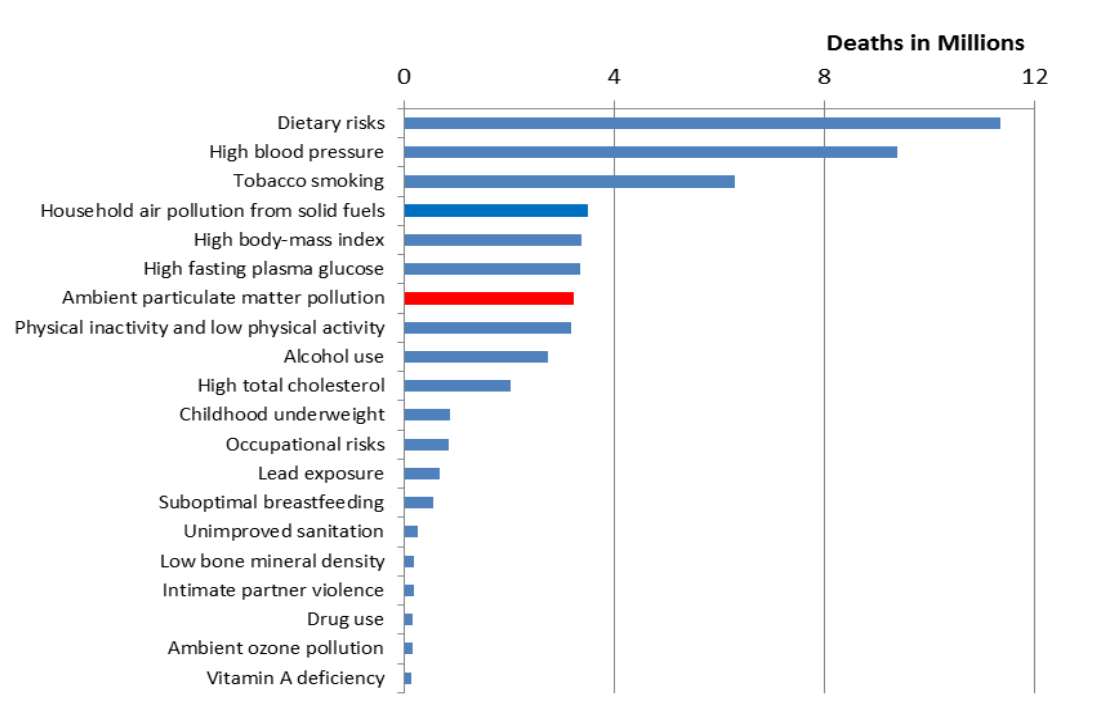
\includegraphics[scale=0.5]{gbd_air_pollution}
\caption{20 Leading Risk Factors Contributing to Deaths Globally in 2010}
\label{fig:gbd_air_pollution}
\end{figure}

However the methods by which exposure to air pollution is estimated are under constant revision. Due to limitations in these methods, epidemiologists may therefore be making misleading or incorrect conclusions.\hfill

The matter of presenting and interpreting data in this field in the opinion of the author, can be confusing and hard to interpret by lay-people. Given better information and understanding of air pollution, would the public change their behaviour and therefore lower their exposure? Possibly leading to health benefits?\hfill

This transfer report begins by giving a general introduction to the subject of air pollution, it's health effects, and how health studies of air pollution have estimated population exposure in the past. It then conducts a more detailed review of dynamic exposure-health studies and the ways in which geographic information systems and science (GIS) have been used in this field. This sets the scene for novel research into personal exposure of the population of London and the ways in which GIS can be used to further this field, and the understanding of the implications.\hfill
\label{chap:intro}

\chapter{Background}
\section{Air pollution - sources and behaviour}
\label{sec:whatisairpollution}

\subsection{What is air pollution?}
\label{subsec:whatisairpollution}
Air pollution is defined by \cite{colls1997} as "material emitted into the air from stationary or mobile sources, moving subsequently through an aerial path and perhaps being involved in chemical or physical transformation before eventually being returned to the surface". This thesis focuses on the places in which humans, particularly in urban environments, are exposed to this pollution.

%%%%%%%%%%%%%%%%%%%%%%%%%%%%%%%%%%%
%%% PARTICLE TYPES AND SIZES
%%%%%%%%%%%%%%%%%%%%%%%%%%%%%%%%%%%

\subsection{Particle types and sizes}
\label{subsec:particletypesandsizes}

Air pollution is a summary term for many sub-categories of pollutants. Pollutants can be solid particles, liquid particles, or gaseous material. They can also be classified as either a primary or secondary pollutant. For example fumes emitted from the stack of a power station are classified as primary pollutants, whereas low-level (ground level) ozone formed by chemical reactions between primary pollutants catalysed by sunlight are classed as secondary pollutants. The UK Department for Environment, Food and Rural Affairs (DEFRA) summarises the main constituents of air pollution and their typical sources as follows (\cite{DEFRA2011}):

\begin{itemize}
\item Particulate matter
\begin{itemize}
\item Combustion (traffic or stationary sources), sea-spray, construction, quarrying.
\end{itemize}
\item Oxides of nitrogen (NO$_{x}$)
\begin{itemize}
\item Combustion. Road transport, electrical supply industry, other industry.
\end{itemize}
\item Ozone (O$_{3}$)
\begin{itemize}
\item A secondary pollutant, not emitted directly from human-made sources, but formed as a result of reactions between other pollutants (NOx, VOCs) in sunlight.
\end{itemize}
\item Sulphur dioxide (SO2$_{2}$)
\begin{itemize}
\item Combustion of fuels such as coal and heavy oils by power stations.
\end{itemize}
\item Polycyclic aromatic hydrocarbons (PAHs) 
\begin{itemize}
\item Many different sources. DEFRA uses Benzo[a]pyrene as a marker. Main sources are coal and wood burning, fires, industrial processes. Traffic combustion (diesel inparticular) is a major contributor.
\end{itemize}
\item Benzene
\begin{itemize}
\item Domestic and industrial combustion and road transport.
\end{itemize}
\item 1,3-butadiene
\begin{itemize}
\item Combustion of petrol i.e. motor vehicles that use petrol as a fuel source
\end{itemize}
\item Carbon monoxide (CO)
\begin{itemize}
\item Occurs from incomplete combustion of fuels that contain carbon. Road transport, residential combustion and industrial combustion are the main sources.
\end{itemize}
\item Lead (Pb)
\begin{itemize}
\item Combustion of coal and nonferrous metals
\end{itemize}
\item Ammonia
\begin{itemize}
\item Mainly from argiculture such as manure, fertilisers and slurry.
\end{itemize}
\end{itemize}

When discussing the amount of pollutants in the air, either volumetric or gravimetric units are used. Volumetric units quantify the ratio of volume of pollutants to clean dry air ( itself a mixture of nitrogen, oxygen, argon etc. ), whereas gravimetric units  quantify the mass of the material per volume of air. Most laws and guidelines, such as the EU Air Quality Standards (see Section \ref{sec:healtheffects}), use gravimetric measurements. Table \ref{tab:pollution_units} summarises the abbreviations for volumetric and gravimetric units which are used throughout this research.

\begin{table}[H]
\centering
    \begin{tabular}{ | l |}
    \hline 
     \textbf{Volumetric} \\ \hline
      Parts per million of pollutant per parts of air volume (10\textsuperscript{-6} ppm) \\ \hline
     Parts per billion of air pollutant per parts of air volume (10\textsuperscript{-9} ppb) \\ \hline
     Parts per trillion of air pollutant per parts of air volume (10\textsuperscript{-12} ppt) \\ \hline
     \textbf{Gravimetric} \\ \hline
     milligrams of pollutant per cubic metre (mg/m\textsuperscript{3}) \\ \hline
     micrograms of pollutant per cubic metre ($\mu \text{g m}^{-3}$) \\ \hline
     nanograms of pollutant per cubic metre (ng/m\textsuperscript{3}) \\ \hline
    \end{tabular}
\caption{Abbreviations for volumetric and gravimetric pollutant units}
\label{tab:pollution_units}
\end{table}
 
Of the ten pollutants listed above, over half list transport combustion as being a source. When combined with proximity to humans in urban environments it is easy to see why air quality in towns and cities, and in particular the pollutants caused by vehicles in these environments, receives such great interest in the field of air quality research and environmental science.

%%%%%%%%%%%%%%%%%%%%%%%%%%%%%%%%%%%
%%% URBAN ENVIRONMENTS
%%%%%%%%%%%%%%%%%%%%%%%%%%%%%%%%%%%

\subsection{Urban environments}
\label{subsec:urbanenvironments}
In many cities around the world hundreds of thousands of people now live within metres of major pollution sources such as car-filled roads, power stations or industrial plants. Due to increasing urbanisation this is rising. According to the World Health Organisation (WHO), as of 2010, more than 50\% of the world’s population live in urban areas. This is up from 40\% in 1990. The prediction is that by 2050 this number will rise to 70\% (\cite{GlobalHealthObservatory2012}). As the numbers of people living in cities has grown, so has the infrastructure required to support them; much of which causes air pollution. High numbers of people are now being exposed to air pollution above WHO guidelines during their normal day to day activities. Given this close link between population density and pollution, it is important to understand the complexity of air pollution in urban environments.

In 2012 WHO published a review which summarised data on particulate matter levels in major cities across the world. The data were split into two categories, particulate matter of a diameter of less than 2.5 micrometres (referred to as PM$_{2.5}$) and particulate matter of a diameter of less than 10 micrometres (referred  to as PM$_{10}$)  (\cite{WorldHealthOrganization2012}). Although the health effects of poor air quality will be discussed in Section \ref{sec:healtheffects}, to provide immediate context, we can refer to WHO Factsheet no. 313 which gives the following numbers as limits for 'acceptable and achievable PM levels to minimise health effects in the context of local constraints' (\cite{WorldHealthOrganization2011}). NO2 values are also included for future reference.

\begin{table}[H]
\centering
    \begin{tabular}{ | l | l | l |}
    \hline 
     & Annual mean ($\mu \text{g m}^{-3}$) & 24 hour mean ($\mu \text{g m}^{-3}$) \\ \hline
     PM$_{2.5}$ & 10 & 25\\ \hline
     PM$_{10}$ & 20 & 50\\ \hline
     NO$_{2}$ & 40 & 200\\ \hline
    \end{tabular}
\caption{Table of 'acceptable' WHO PM and NO$_{2}$ levels}
\label{tab:whopmlevels}
\end{table}

Figure \ref{fig:mapofpm10} shows the annual average PM$_{10}$ levels for each major world city for 2003-2010, weighted by population, from the same WHO review.

\begin{figure}[H]
\centering
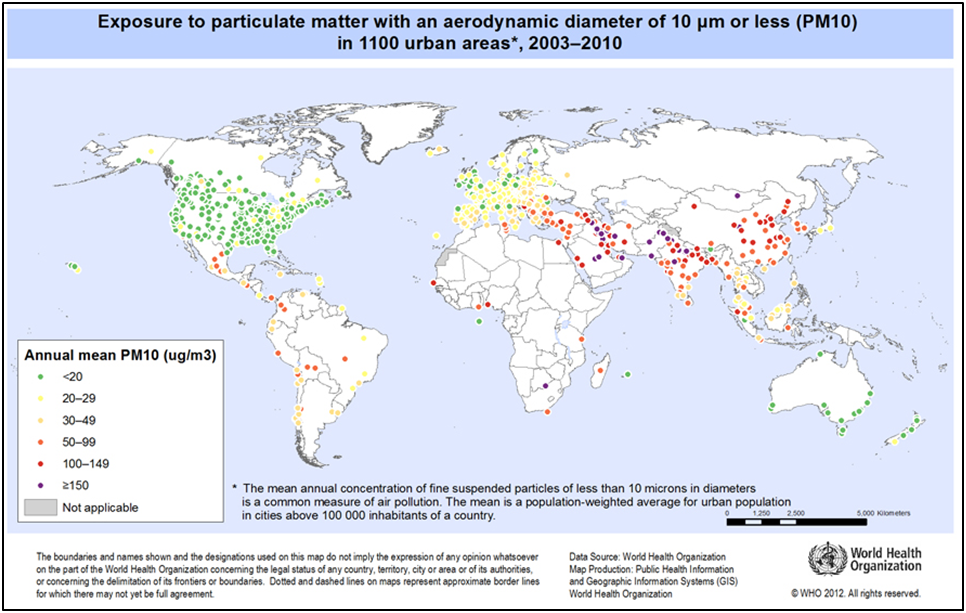
\includegraphics[scale=0.8]{images/who_pm10_world_map}
\caption{A map of PM$_{10}$ in major world cities}
\label{fig:mapofpm10}
\end{figure}

As can be seen, there are many urban areas where the WHO annual mean for PM$_{10}$ is exceeded. By way of example we can consider Beijing (39.913889 N, 116.391667 W) which has a population of 15.59m and is China's second largest city (\cite{TheUnitedNationsStatisticsDivision2013}), is subject to seasonal dust storms, hot humid summers and cold dry winters - and suffers from severe air pollution problems. During the 1990s attempts were made at controlling air pollution in the city by introducing the use of low-sulphur coal, using natural gas as an alternative to coal, phasing out leaded petrol, and moving factories and heavy industry outside of the city. However, due to increasing vehicle numbers and the rapid growth of the industrial sector, particle levels continued to remain higher than national standards (\cite{Sun2004}). The nearby area of Hebei Province (which rings Beijing and is heavily industrial) made the efforts of the government to control air quality in Beijing even more difficult as the Hebei region has lower fuel quality standards, and emissions frequently drift into Beijing (\cite{Tuo2013}) due to prevailing winds (Meteorology is discussed in Section \ref{subsec:meteorology}).

During the early 21$^{st}$ century the use of air pollution monitoring equipment became more commonplace and better data was collected to enable scientists to understand the issues that Beijing (and similar urban environments) faced. \cite{Sun2004} found that during the years 1999 and 2000, PM$_{2.5}$ concentrations were in the range 37 -- 357 $\mu \text{g m}^{-3}$ , and estimated a yearly average of 89.7 $\mu \text{g m}^{-3}$.  The research concluded that coal burning and traffic exhausts, along with dust from long range sources, were the major pollution sources in the urban environment of Beijing (\cite{Sun2004}).

The study of pollution in urban environments is essential as these areas are where humans are most readily exposed and they are where the sources of emissions are most frequent. Although PM has been discussed here, similar issues apply to other traffic linked pollutants such as NO$_{x}$ and PAHs. There are also other factors, other than the type of pollutant, that complicate the understanding of pollution in urban environments, such as weather and geography. Within these urban environments there are hyper-local conditions that can raise and lower levels. These notions are explored in sections \ref{subsec:meteorology}, \ref{subsec:urbantopography}, \ref{subsec:microenvironments} and \ref{subsec:trafficpollution}.

%%%%%%%%%%%%%%%%%%%%%%%%%%%%%%%%%%%
%%% Meteorology
%%%%%%%%%%%%%%%%%%%%%%%%%%%%%%%%%%%

\subsection{Meteorology}
\label{subsec:meteorology}

Local weather conditions have a strong influence on air quality.
%%%RAIN
Air pollution can be removed from the air in the process of cloud formation, and then deposited on the ground when the clouds turn to rain at a future time and/or place. Falling rain can also remove pollutants from the air by collecting the pollution and 'cleaning' the air as it falls. Both of these processes are grouped into the term 'wet deposition'. A 6 $\mu \text{g m}^{-3}$ difference in PM$_{10}$ was observed in Edinburgh between days with no rainfall compared to those with more than 20mm of rain (\cite{DEFRA2007}). In December 2013 it was even reported that China was considering using 'cloud seeding', i.e. the process of engineering the weather to rain, as a method to lower air pollution in the most polluted regions of China (\cite{Slezak2013}).

%%%WIND DISPERSION & DILUTION
Wind can effect air quality by trapping or recirculating air pollution (discussed in Section \ref{subsec:urbantopography}), but can also disperse the pollution or move it to entirely new areas. Pollutants emitted in one area can often have their impact on the air quality in other areas due to transportation by air currents. This notion was first proposed in the 1960s when studying the acidification of lakes in Scandinavia \cite{Summers1976}, where it was theorised that the high acid levels were due to air quality elsewhere in Canada. Depending on the lifetime and properties of a pollutant, it can be transported on scales ranging from the street level to the global scale (\cite{Monks2009}). \cite{Stohl2003} found gases were being transported from North America to Europe. More locally, an odour event in the South-East of England on 18 April 2008 (\cite{TheGuardian2008}) was found to have originated from agricultural emissions in northern Germany (\cite{Smethurst2012}). The Geneva Convention on Long-range Trans-boundary Air Pollution was established in 1979 to look at ways to deal with this movement of air pollution between borders in terms of national air quality guidelines and limits, and came into force in 1983 (\cite{UnitedNationsEconomicCommissionforEurope1983}). Wind can also dilute air pollution, though this varies by pollutant. NOx concentrations were found to have halved at a monitoring station in Hillingdon, UK when wind speed rose from 5 to 10 m/s-1, while PM$_{2.5}$ also decreased, however the coarse PM (PM$_{2.5 - 10}$) increased due to re-suspension of particles that had previously settled (\cite{DEFRA2007}).

%%% TEMPERATURE
Direct sunlight (UV radiation) and higher temperatures, on hot summer days, can initiate reactions with nitrogen dioxide which can lead to the formation of ozone. The ozone and ozone forming chemicals remain in the atmosphere and can be transported over regional and national borders. This layer can then settle over cities such as London and lead to what is often referred to as summertime 'smog'. The South-East of England often has high concentrations during spring and summer as, amongst other sources, it is close to European pollution sources (\cite{LondonAir}). Although vehicle emissions of nitrogen oxide can have the effect of reacting with the ozone to lower the level of ozone in areas where vehicle emissions are particularly high. (\cite{EnvironmentalProtectionAgency2012}).

%%%%%%%%%%%%%%%%%%%%%%%%%%%%%%%%%%%
%%% Urban topography
%%%%%%%%%%%%%%%%%%%%%%%%%%%%%%%%%%%

\subsection{Urban topography}
\label{subsec:urbantopography}

In the urban environment, streets are often bordered by tall buildings which can influence pollution levels for people at ground level. Topography of this nature is often referred to as a 'street canyon'. In extreme circumstances such as on the streets of Hong Kong, skyscrapers are littered throughout the city, but on smaller scales such as Oxford Street (London, UK) similar issues occur but with modest building heights. Being bordered by tall buildings creates a sheltering effect from the wind, stopping particles being moved elsewhere. The typical street-canyon effect occurs when there is a steady flow over the top of tall buildings (see figure \ref{fig:street_canyon}), where the mean flow is perpendicular to the direction of the street (\cite{Britter2003}). With roof-level wind-speeds of 1.5-2 m/s, the air is recirculated within this 'box' and air quality deteriorates as sources (usually traffic) emit more fumes.

\begin{figure}[H]
\centering
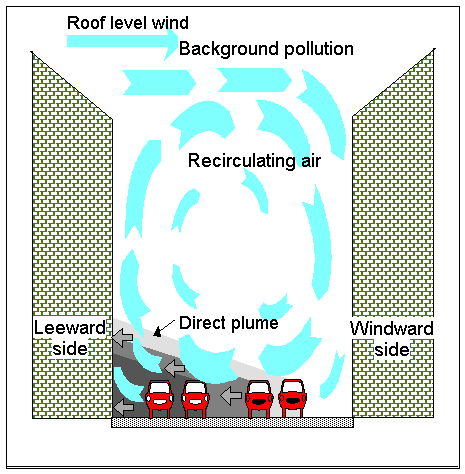
\includegraphics[scale=0.7]{street_canyon}
\caption{Pollutant dispersion in a regular street canyon}
\label{fig:street_canyon}
\end{figure}

Mexico City is an example of a city that is subject to this effect on a large scale. Situated in central Mexico, North America (19.4328° N, 99.1333° W), Mexico City is one of the most populated cities in the world and has an estimated population of about 21m (2011) living within the Mexico City Metropolitan Area (MCMA) of 1,485 km\textsuperscript{2} (\cite{TheUnitedNationsStatisticsDivision2013}). Mexico City is located in the crater of a large extinct volcano, which means that the entire city suffers from the aforementioned canyon effect. Almost like it is surrounded by skyscrapers. This is exacerbated by a fleet of older vehicles with poor engines (the effects of which are discussed more in Section \ref{subsec:trafficpollution}), low levels of oxygen (due to the high altitude of the city), and wind patterns that concentrate pollutants in the western and southern parts of the city (\cite{Garza1996}) where the population is most dense.

To summarise, air pollution in the urban environment can be effected by the meteorology and topography of the area. On the smaller scale than 'area' there are also micro-environments that people spend time in, for example inside a bus, which can exhibit very different characteristics than the rest of the city or even street.

%%%%%%%%%%%%%%%%%%%%%%%%%%%%%%%%%%%
%%% Micro-environments
%%%%%%%%%%%%%%%%%%%%%%%%%%%%%%%%%%%

\subsection{Micro-environments}
\label{subsec:microenvironments}
Micro-environments are defined as the immediate small-scale environment of an organism, especially as a distinct part of a larger environment. Examples in the context of this thesis include the air quality inside a vehicle, a house or  underground train carriage, in the context of the environment outside. Understanding how pollutant levels change in these micro-environments is key, as much of our time is spent within these environments, thus our exposure level to air pollutants whilst in them could have important impacts on our health.

%%%%%%%%%%%%%%%%%%%%%%%%%%%%%%%%%%%
%%% Indoors
%%%%%%%%%%%%%%%%%%%%%%%%%%%%%%%%%%%
\subsubsection{Indoors}
\label{subsubsec:indoors}

The most common micro-environment is within buildings, the air we are exposed to when we are at home, in the office or at school etc. WHO calculated in 2005 that people spend 89\% of their time indoors (\cite{WorldHealthOrganization2005}). In these environments, people are exposed to pollutants generated outdoors that penetrate to the indoor environment, as well as to pollutants produced indoors.

The EXPOLIS study examined how much time people spend in these environments by asking 1427 people across their European project partners to complete activity diaries. They found that the amount of time people spend indoors varied by whether the people were employed or not, in what type of job, whether they lived alone and/or whether they had children. Gender and season of year were also found to be factors. By bringing together some of the figures from their study, it can be calculated that the mean number of hours that people spend indoors, not taking account of any other adjustment factors, was 20.66 hours per day (\cite{Schweizer2007}). So understanding indoor air quality, which would include filtration of outdoor air into the building as well as pollutants whose sources are inside, is important in understanding personal exposure.

However research on indoor pollution has not had the same focus as outdoor pollution for a number of reasons. Firstly the perceived need to deal with coal and traffic emissions, the ease of monitoring outdoor pollution using fixed monitoring sites (compared to monitoring every home). Secondly epidemiologists have traditionally only linked outdoor pollutant concentrations to health health issues, furthermore, legislating the air that people can breathe in their own homes can be seen as intrusive to people's private lives, finally  the funding and policy initiatives around air pollution research has mainly come from developed countries, which who do not have such an issue with indoor pollution as developing countries (\cite{WorldHealthOrganization2010}) (due to developing countries using solid fuel for cooking and heating inside their homes more).

The pollutants that are emitted indoors, and which the US Environmental Protection Agency (EPA) focus on in their guide to indoor air pollution, include Volatile Organic Compounds (VOCs), carbon monoxide and nitrogen dioxide (\cite{UnitedStatesEnvironmentalProtectionAgency2008}). VOCs in indoor air come mostly from products used around the house such as paint, varnish, cleaning sprays, air fresheners and pesticides but can also be emitted by building materials and furnishings. Carbon monoxide and nitrogen dioxide on the other hand are more commonly associated with the use of indoor furnaces, gas cookers, gas heaters, leaking chimneys and people smoking tobacco indoors.

The EPA report however, only focuses on indoor air pollution relevant to buildings in the US. In different parts of the world indoor air quality varies in terms of the pollutants and the impact, especially in Asian countries where less clean combustion fuels are often used for cooking in the home and the numbers of people that smoke while indoors is greater (\cite{Lee2010}). 
\cite{Baumgartner2011} sampled PM$_{2.5}$ in 44 kitchens of the Yunnan area of China in 2010, where 95\% of the kitchens used wood or crop residue for cooking, and 96\% used a mix of wood-charcoal and wood or crop reside for heating. During the summer months, when the sampling was done, mean concentrations were found to be around 107 $\mu \text{g m}^{-3}$. So presumably would be higher during the winter when the windows are likely to be closed and air cannot escape as easily. Similarly, \cite{Li2011} compared pollutant concentrations in kitchens in relation to different types of stoves in Peru. Means of 181 $\mu \text{g m}^{-3}$ and 3.5 ppm were found for the open-pit stoves for PM$_{2.5}$ and CO respectively. In a larger study across 168 venues in China, Japan, Korea, Malaysia, Pakistan and Sri-Lanka, PM$_{2.5}$ measurements were made and an average indoor level of 137 $\mu \text{g m}^{-3}$ was found (smoking venues were 156 $\mu \text{g m}^{-3}$, non-smoking venues were 34 $\mu \text{g m}^{-3}$).

Poor indoor air quality is not always due to indoor sources. The pollutant levels outside an indoor environment has been found to have an impact, although this is dependant on many mitigating factors such as the buildings air filtration units, proximity to outdoor sources, and wind speed/direction. In North America, homes close to Ambassador Bridge (Detroit) were measured over five 24 hour periods and they found that ambient black carbon concentrations significantly contributed to indoor concentrations regardless of wind speed \cite{Baxter2008}. In Osaka, Japan fine PM (PM$_{2.5}$) was significantly correlated with fine PM outside the properties and it was estimated that about 30\% of indoor PM$_{10}$ particles were from diesel exhausts from nearby roads (\cite{Funasaka2000}). In Europe (Prague, Czech Republic) PM$_{2.5}$ was sampled in a school gym during 2005 and 2006, and levels were found to be similar to a nearby fixed-site monitor (24.03 compared to 25.47) (\cite{Branis2009}).

%%%%%%%%%%%%%%%%%%%%%%%%%%%%%%%%%%%
%%% In-vehicle
%%%%%%%%%%%%%%%%%%%%%%%%%%%%%%%%%%%
\subsubsection{In-vehicles}
\label{subsubsec:invehicle}

The air quality people are exposed to between these indoor micro-environments, when travelling, can differ greatly from general ambient concentrations. Similarly, when space inside vehicles has its own air quality micro-environment. Conditions can be affected by having windows open or closed, the type of vehicle, and the vehicle's location amongst other factors. \cite{Adams2001} measured PM$_{2.5}$ during 465 journeys in London over a three week period, at peak and off-peak times of the day during the summer of 1999 and winter of 2000.

\begin{table}[H]
\centering
    \begin{tabular}{ | l | l |}
    \hline 
     \bfseries{Transport mode} & \bfseries{Mean ($\mu \text{g m}^{-3}$)} \\ \hline
     Bus & 39.0\\ \hline
     Car & 37.7\\ \hline
     Underground tube & 247.2\\ \hline
     Overground tube & 29.3\\ \hline
    \end{tabular}
\caption{PM$_{2.5}$ by transport mode from \cite{Adams2001}}
\label{tab:adams_transport_means}
\end{table}

They observed a great deal of variability between travel modes (see table \ref{tab:adams_transport_means}), and against typical ambient PM$_{2.5}$ levels (around 10-30 $\mu \text{g m}^{-3}$) recorded for central London. Outside of London, also in 1999/2000, \cite{Gulliver2004} conducted in-vehicle monitoring along a stretch of road in Northampton (80 km North/North West of London). They also observed elevated levels of particulates inside the vehicle (table \ref{tab:gulliver_vehicle_means}).

\begin{table}[H]
\centering
    \begin{tabular}{ | l | l |}
    \hline 
     \bfseries{PM Fraction} & \bfseries{Mean ($\mu \text{g m}^{-3}$)} \\ \hline
     PM$_{10}$ & 43.16\\ \hline
     PM$_{2.5}$ & 15.54\\ \hline
    \end{tabular}
\caption{In-vehicle PM from \cite{Gulliver2004}}
\label{tab:gulliver_vehicle_means}
\end{table}

Neither of these authors comment on air quality inside vehicles or the resultant exposure. They only conclude that in-vehicle pollutant concentrations cannot be taken to be the same as outdoor values. The situation is further complicated by additional variables such as whether windows are open or closed, the speed of the vehicle, or the number of people inside the vehicle.

%%%%%%%%%%%%%%%%%%%%%%%%%%%%%%%%%%%
%%% TRAFFIC POLLUTION
%%%%%%%%%%%%%%%%%%%%%%%%%%%%%%%%%%%

\subsection{Traffic pollution}
\label{subsec:trafficpollution}

%%% THE NUMBERS OF VEHICLES HAS CHANGED DEPENDING ON WHERE IN THE WORLD YOU LOOK
Between the years of 1950 and 1994, there was a dramatic increase in vehicle traffic on the worlds roads.  Vehicle numbers increased from 53 million, to 460 million in the space of 44 years. However, this rate of growth was not uniform around the world (\cite{schwela2002}). The rate slowed considerably in industrialised countries, but population growth and increased urbanisation and industrialisation accelerated the use of vehicles elsewhere (see figures \ref{fig:europe_vehicles_per_1000} and \ref{fig:china_malaysia_brazil}) (\cite{DepartmentforTransport2012}).

\begin{figure}[H]
\centering
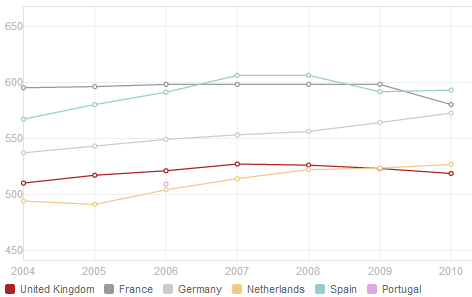
\includegraphics[scale=1]{europe_vehicles_per_1000}
\caption{Vehicles per 1000 people from \cite{TheWorldBank2013}}
\label{fig:europe_vehicles_per_1000}
\end{figure}

\begin{figure}[H]
\centering
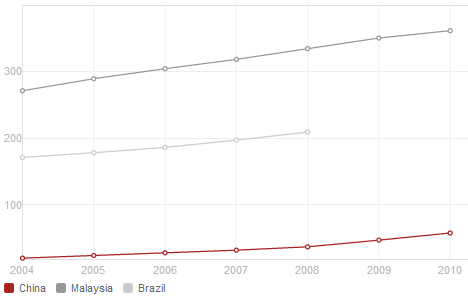
\includegraphics[scale=1]{china_malaysia_brazil}
\caption{Vehicles per 1000 people from \cite{TheWorldBank2013}}
\label{fig:china_malaysia_brazil}
\end{figure}

Against this backdrop of increasing numbers of vehicles, there is emerging evidence that traffic emissions are harmful to human health. In 2010 the US Health Effects Institute (HEI) published the findings of a systematic review of evidence about traffic pollution, and whilst noting that there were many areas still needing further research, there was evidence to support a casual relationship between exposure to traffic-related air pollution and asthma (\cite{HPotHEoT-RA2010}). Toxicological research has now also started to link not only traffic emission pollutants, but also non-exhaust pollutants such as road abrasion, tyre wear and brake wear to adverse health effects (\cite{WorldHealthOrganization2013}). The latter being particularly significant given that there are no laws which consider this element of traffic pollution and therefore no guidelines or limit values. Despite this, measuring and defining pollution solely from traffic sources in the urban environment is technically difficult, which makes linkages with exposure estimates and health effects problematic. Different studies have therefore used different pollutants as markers for traffic emissions. Epidemiological studies have often used NO$_{2}$ as a marker for combustion-related pollutants, in particular those emitted by road traffic or indoor combustion sources (\cite{WorldHealthOrganization2010}). More recently black carbon has started to become the standard way of measuring diesel emissions due to it's relative ease of measurement using optical techniques such as micro-aethalometers.

%%% LET'S LOOK AT BEIJING AS A CASE STUDY AND SEE A BIT MORE ABOUT TRAFFIC POLLUTION
Taking the city of Beijing as example again, in 2008 the Olympic Games were held there and this heightened the world’s interest in Beijing's air quality and put the issue under national scrutiny. Global newspapers focused on the effects that poor air quality might have on the performance of the athletes. The reporter James Reynolds of the BBC wrote "\textit{China is spending billions of pounds on new roads, new venues and on perfect celebratory shows but all that may come to nothing unless this city cleans up its air}" (\cite{BBC2007}). Under this pressure, to try and bring air quality problems under control (at least in the short term while the Olympics were taking place) the Beijing Government implemented a number of measures in the run-up to the games. Stricter vehicle emission standards were adopted, better public transport infrastructure was developed, and from July 2008 to September 2008 a traffic demand management scheme was introduced whereby odd/even vehicle registrations took it in turns to be used on the roads on alternate days (\cite{Wang2009}). This provided an ideal real-world experiment for the local scientists to quantify how much of the areas pollution was due to vehicle emissions. Data on black carbon levels was collected by on-road, fixed background and fixed road-side monitors, and then analysed to investigate whether the scheme had achieved the desired effect.

\begin{figure}[H]
\centering
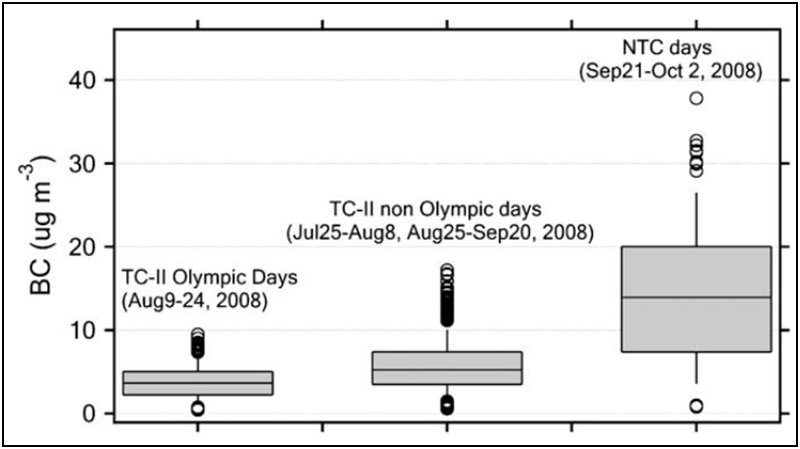
\includegraphics[scale=1]{black_carbon_olympic}
\caption{Black carbon concentrations during 2008 in Beijing from \cite{Wang2009}}
\label{fig:blackcarbonolympic}
\end{figure}

The results from this study are shown in figure \ref{fig:blackcarbonolympic} and demonstrate how mean black carbon concentrations dropped to around 5 $\mu \text{g m}^{-3}$ during the Olympics (second boxplot) compared to around 14 $\mu \text{g m}^{-3}$ after the Olympics (third boxplot). In addition, during the Olympics on days when the main sporting events were happening, there was a further reduction to around 4 $\mu \text{g m}^{-3}$ (first boxplot). The traffic in Beijing, at least within the limits of this small subset of data, seemed to be contributing to around 10 $\mu \text{g m}^{-3}$ of black carbon pollution in the air. The authors of this study go on to conclude that the main source of emissions in Beijing at the time are from traffic, and that the traffic demand management scheme was effective at bringing emissions down to within acceptable (WHO) limits. However this seems to be a simplification of the issue, especially given the impact of factories in the vicinity (discussed in \ref{subsec:urbanenvironments}). Nonetheless, the exposure of the residents of Beijing to pollution, a debatable proportion of which is from tailpipe emissions, is high.

%% Now lets look at a more Western city

In Europe, where factories and heavy industry tend not to be based within urban centres, the proportion of the populations exposure related to traffic emissions is high. Often, due to meteorology (see \ref{subsec:meteorology}), the emissions may also be from other urban centres. For example emissions from outside London are estimated to account for around 40\% of NO$_{2}$ concentrations (with the other 60\% being generated locally) (\cite{GreaterLondonAuthorityGLA2010}. This ratio changes depending on different spatial resolutions. In areas close to roads, the contribution of traffic emissions to overall pollution levels is much higher due to the proximity to sources (vehicles). The effect of traffic emissions as a percentage of airborne pollutants is well demonstrated by a study by \cite{Mayer1999}. Figure \ref{fig:stuttgarttraffic} identifies clear trends related to rises in NO and NO$_{2}$ during morning and evening rush hours on working days.

\begin{figure}[H]
\centering
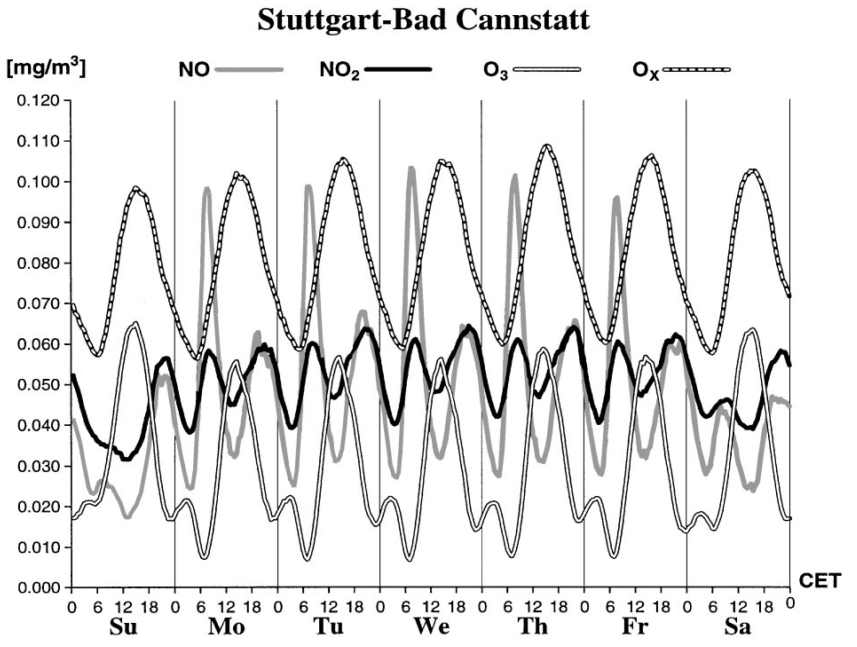
\includegraphics[scale=0.6]{stuttgarttraffic}
\caption{Average weekly and diurnal cycles of NO, NO$_{2}$ ,O$_{3}$ and O$_{x}$ at the urban air-quality station Stuttgart-Bad Cannstatta for the period 1981-1993 from \cite{Mayer1999}}
\label{fig:stuttgarttraffic}
\end{figure}

%% What's going on with policy attempts to reduce.
 
As air pollution from vehicles is harmful to health, and traffic pollution is so prevalent in urban environments, more permanent long-term attempts to reduce traffic pollution are ongoing in most major cities and countries around the world. Though different countries have sought to achieve this in different ways. Professor Williams recent (December 2013) article for the website 'The Conversation' explains how the EU have attempted to legislate to reduce vehicle emissions (\cite{Williams2013}), prompted by the Kyoto Protocol of 1997 which was linked to the United Nations Framework Convention on Climate Change (\cite{UnitedNations1998}). Regarding vehicle emissions the protocol sought to specifically reduce CO$_{2}$ emissions and they did this by insisting that car dealers in new passenger cars must provide potential buyers with useful information on these vehicles' fuel consumption and CO$_{2}$ emissions and this information must be clearly displayed. Limits were placed on CO$_{2}$ emissions, as a ratio of kilometres travelled, to encourage more efficient use of fuel and therefore lower emissions. This legislation encouraged companies making vehicles for the EU markets to invest in the production and marketing of diesel vehicles, as they provide better fuel consumption than petrol vehicles. Europe now has a vehicle fleet which is predominately diesel. The problem with this is that diesel cars emit significantly higher levels of air pollutants than petrol cars fitted with three-way catalytic converters (\cite{Williams2013}). The difference between the two emission levels are even greater when considered in the real-world rather than measured in laboratory conditions (\cite{Carslaw2011}). A study in 2007 estimated that the health effect of favouring diesel vehicles over petrol vehicles had the combined effect of contributing to approximately 1850 additional premature deaths over the period 2001-2020, or around 90 premature deaths per year (\cite{Mazzi2007}).

%% The alternative is different vehicles altogether.
The alternative to both diesel and petrol vehicles are vehicles that produce different types of emissions, or low/no emissions. These are often referred too as ultra-low emission vehicles, such as hybrid or electric. Unfortunately for air quality in urban environments they are currently a very small percentage of new vehicles. In 2013 only 1\% of new registrations in the EU (with some notable exceptions such as 4.5\% in the Netherlands where generous financial incentives have been offered since 2007) were low or no emission vehicles (\cite{Transportation2013}).

%%%%%%%%%%%%%%%%%%%%%%%%%%%%%%%%%%%
%%% Summary of what is air pollution
%%%%%%%%%%%%%%%%%%%%%%%%%%%%%%%%%%%
\subsection{Summary}
\label{subsec:whatissummary}

Section \ref{sec:whatisairpollution} introduced the subject of air pollution. It was considered as non-naturally occurring material in the air, or material which has had it's composition or levels altered by non-natural sources. It can take many different forms and be categorised in different ways, for example particulate matter, nitrogen oxides, ozone or sulphur dioxide. It was discussed how many of the causes of air pollution are linked to vehicle combustion engines and that in urban environments, where people are increasingly living, this places the sources and public in close proximity to each other. This can be affected (both positively and negatively) by different meteorological conditions and the topology of the region, city, and even individual streets and buildings. Within these environments, it was explained that there are micro-environments such as inside vehicles and buildings which can also raise or lower pollution levels. As this research intends to focus on urban environments, traffic emissions were then considered in a little more detail. The Beijing Olympics 2008 was used as a case-study to understand the impact that traffic emissions can have on air quality in a major city, and the diesel dominated vehicle fleet of Europe was then explained (touching on the impact compared to petrol that this has had on air quality).

Now that the subject of air pollution has been introduced, the next section of this background will give an overview of the impact on human health from air pollution i.e. why Section \ref{sec:whatisairpollution} actually matters to us.

\newpage
%%%%%%%%%%%%%%%%%%%%%%%%%%%%%%%%%%%%%%%%%%%%%%%%
%%% AIR POLLUTION AND HEALTH SECTION %%%%%%%%%%%
%%%%%%%%%%%%%%%%%%%%%%%%%%%%%%%%%%%%%%%%%%%%%%%%
\section{Health effects of air pollution}
\label{sec:healtheffects}

\begin{quote}
"Clean air is considered to be a basic requirement of human health and well-being. However, air pollution continues to pose a significant threat to health worldwide" (\cite{WorldHealthOrganisation2006}).
\end{quote}

\subsection{An overview}
\label{subsec:anoverview}

%%%%%%%%%%%%%%%%%% Where concerns about air pollution and health came from

%https://www.hsph.harvard.edu/news/press-releases/air-pollution-premature-death-u-s-seniors/
%“We found that the mortality rate increases almost linearly as air pollution increases. Any level of air pollution, no matter how low, is harmful to human health.”

From the 1600’s onwards coal was the main source of heat and energy in major UK cities. Concern from the scientific community and coherent programs of research about the possible negative effects of this fuel source were limited. When undertaken the research often focused on poor visibility or damage to buildings rather than human health. It was the early 1900’s when coherent and robust studies began to investigate mortality and links to ‘fog’, as it was known at the time. Notably with Russell’s paper \textit{'The Influence of fog on mortality from respiratory diseases'} being published in The Lancet in 1926 (\cite{Russell1926}) . This publication preceded London's 'Great Smog' of 1952, which was one of the UK's most important air pollution events in history in terms of realisation of the links between pollution and health. Research conducted since this event has had a great impact on the study of air pollution, public perception and government regulation to combat it. Data at the time showed that a rise in fog (pollution) levels was closely followed by rises in mortality and morbidity (\cite{Bell2003}). At the time it was estimated that between 3,500 and 4,000 more people died than would have normally been the case in this period (See figure \ref{fig:greatsmogdeaths} from \cite{GreaterLondonAuthorityGLA2002}). The rise in mortality was originally attributed to influenza, however sensitivity analysis by \cite{Bell2003} revealed that only an extremely severe influenza epidemic could have accounted for the excessive deaths recorded for that period. Subsequent reanalysis of the data estimated that between December 1952 and March 1953 there were actually 13,500 more deaths than during the same time period the previous year, attributable to (controlling for temperature and influenza) rather than the 3000--–4000 generally reported for the episode.

\begin{figure}[H]
\centering
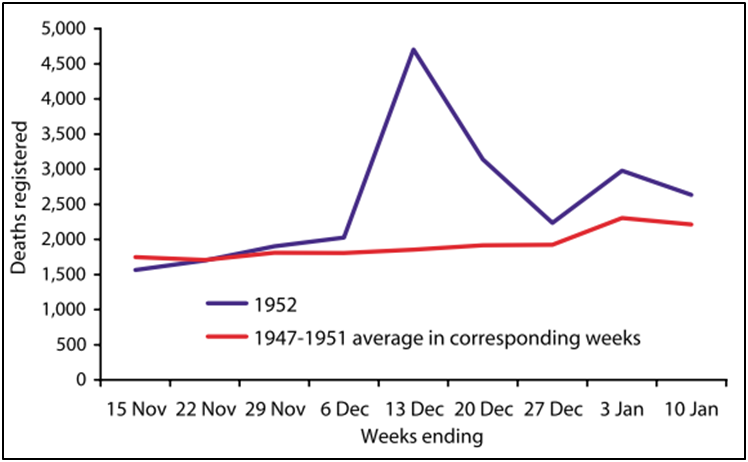
\includegraphics[scale=1.2]{great_smog_deaths}
\caption{Recorded deaths comparison during 'Great smog' period from \cite{GreaterLondonAuthorityGLA2002}}
\label{fig:greatsmogdeaths}
\end{figure}

%%%%%%%%%%%%%%%%%% Some laws and EU regs were passed over time

Once this explicit link between air pollution and health became apparent, laws and regulations began to be written and passed. For example the Clean Air Act in 1956 (with various revisions over time, notably in 1968), the 1970 EC Directive (70/220/EEC), the 1974 Control of Pollution Act and the 1979 International Convention on Long Range Transboundary Pollution.
%%%%%%%%%%%%%%%%%% Now widely accepted that it's harmful to health
It is now widely accepted that air pollution has harmful effects on human health (\cite{WorldHealthOrganization2013}. Although in the Western world, the sources of pollution have shifted from using coal for heating and cooking, to be dominated by combustion engines in vehicles and similar (as discussed in Section \ref{subsec:trafficpollution}).


%%%%%%%%%%%%%%%%%% Epidemiology is _______. Looks at risk factors between exposure and health effects. Allows large scale effects to be examined across populations. Although it can be confusing in the variation, 
When considering the effects of air pollution on public health, studies on large groups of people (tens of thousands plus) often use epidemiological methods. Studies using epidemiological methods will be discussed many times during this thesis, therefore a brief definition of epidemiology and the key terms are now given.

Epidemiology is the the study of how often disease/poor health occurs in a group of people, and the factors that lead to it. Or, more technically defined by Bonita in a WHO publication as \textit{'the study of the distribution and determinants of health-related states or events in specified populations, and the application of this study to the prevention and control of health problems'} (\cite{Bonita2006}). Some key terms include (adapted from \cite{U.S.DepartmentofHealth&HumanServices2014}):

\begin{itemize}
\item Incidence: The number of new ill people in the population over a specified time period
\item Prevalence: The existing number of ill people in the population over a specified time period.
\item Burden of disease: The total significance of the disease or illness to wider society. For mortality this is often measured in years of life lost.
\item DALY (Disability-Adjusted Life Year): A statistic to represent the health of a population. One DALY represents one lost year of healthy life and is used to estimate the gap between the current health of a population and an ideal situation in which everyone in that population would live into old age in full health.
\end{itemize}

%%%%%%%%%%%%%%%%%% Using epidemiology-like studies, health issues from air pollution include x, y, z. Also recently IARC cancer stuff.
Epidemiological studies have '\textit{For decades [ ... ] been a cornerstone of our approach to investigating the health effects of air pollution and have been a principal basis for setting regulations to protect the public against adverse health effects}' \cite{Zeger2000}. Recent high profile examples that look at air pollution include, but are not limited to; respiratory problems (\cite{Peacock2011}), cardiovascular issues (\cite{Brook2010}) and cancer (\cite{Iii2012}, \cite{loomis2013}). Indeed, recently (17 October 2013), the International Agency for Research on Cancer (IARC) classified outdoor air pollution as carcinogenic to humans (\cite{loomis2013}). In an IARC press-release, Dr Kurt Straif, Head of the Monographs Section stated \textit{"The air we breathe has become polluted with a mixture of cancer-causing substances. We now know that outdoor air pollution is not only a major risk to health in general, but also a leading environmental cause of cancer deaths"}.

%%%%%%%%%%%%%%%%%% The strongest association found thus far is between poor health and PM2.5

However as discussed in Section \ref{subsec:particletypesandsizes}, the term 'air pollution' covers a myriad of different pollutants. Thus it is important to untangle which pollutants are more or less harmful to health. This will potentially help people avoid areas with pollution that is most harmful, and help politicians and public sector workers to develop policies that are most effective at reducing the most harmful types of pollution. At present research in this area is underway to fully answer which pollutants are most harmful to health. Evidence points towards short-term exposure to PM$_{10}$ as having negative health effects, but long-term exposure to PM$_{2.5}$ is a stronger risk factor for mortality (\cite{WorldHealthOrganization2013a}, \cite{Dockery1993}). Hence, a broad overview of epidemiological studies of the health effects of air pollution that consider PM$_{2.5}$ will now be discussed.

%%%%%%%%%%%%%%%%%% Across the world it causes X premature deaths
Worldwide, WHO estimate that PM$_{2.5}$ causes about 9\% of lung cancer deaths, 5\% of cardiopulmonary deaths, and 1\% of respiratory infection deaths (\cite{WorldHealthOrganization2012}). In 2013 the Global Burden of Disease publication ranked exposure to air pollution and particulate matter as one of the top ten risk factors for health globally, estimating that over 430,000 premature deaths and around 7 million years of healthy life were lost in Western, Central and Eastern Europe in 2010 from exposure to fine particulate matter (\cite{Brauer2012}) n.b. fine refers to particulate matter smaller than 1 micron in diameter, ultrafine smaller than 2.5 microns (includes the 1 micron particles), and coarse smaller than 10 microns (includes the 1 and 2.5 micron particles). 

In a study looking at PM$_{2.5}$ and anthropogenic ozone, \cite{Silva2013} recently modelled ozone and PM$_{2.5}$ surface concentrations for the entire world, then used concentration-response functions for long-term exposure and mortality (from an American Cancer Society publication) to estimate that annually and globally there are about 2.1 million premature deaths from respiratory problems linked to PM$_{2.5}$, with these being split 93:7 between cardiopulmonary disease and lung cancer (\cite{Silva2013}).

We can therefore see that the health effects of PM$_{2.5}$, when taken in context of large populations are significant. However, these figures are likely to be the tip of a much larger concern as most do not include morbidity i.e. poor health and detriments to the populations quality of life that do not result in death. This is illustrated by figure \ref{fig:airpollutionpyramid} (\cite{Mannino2000}) showing a greater number of the population have less severe health effects that still have a burden on public well-being.

\begin{figure}[H]
\centering
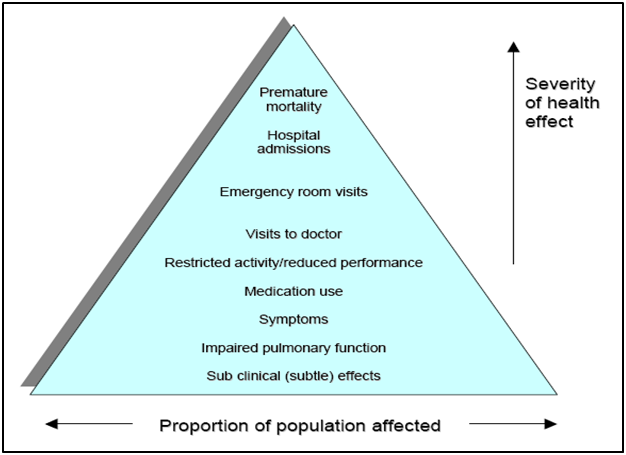
\includegraphics[scale=1.4]{air_pollution_pyramid}
\caption{Air pollution health effects pyramid}
\label{fig:airpollutionpyramid}
\end{figure}

%%%%%%%%%%%%%%%%%% In the UK we have COMEAP. Some estimations on air pollution/health impact are mentioned.

In the UK, COMEAP (the Committee on Medical Effects of Air Pollutants) has been set-up to provide advice to the government and related agencies via the Department of Health's Chief Medical Officer on the harmful effects of air pollution. COMEAP regularly publish reports summarising findings into the health effects of pollutants. In their 2010 report on mortality, they estimated that around 29,000 deaths in the UK in 2008 were attributable to PM$_{2.5}$ (\cite{CommitteeontheMedicalEffectsofAirPollution2010}). Expressing this differently, they estimated that air pollution may have contributed to the earlier deaths of about 200,000 people in 2008, with an average loss of life of about two years per death affected. Also on a UK scale, \cite{Yim2012} estimated that PM$_{2.5}$ causes about 19,000 premature deaths in the UK and 3,200 in London. Note that the reason for these figures being lower than that of COMEAP is that this study focused solely on the deaths attributable to traffic emissions rather than all sources (and gives at least in this context a rough idea of the impact of traffic emissions compared to non-traffic emissions).


On a more regional level, \cite{Miller2010} used life-tables and concentration-response coefficients to estimate deaths attributable to PM$_{2.5}$ to be 4,267 in Greater London for 2008.

%%%%%%%%%%%%%%%%%% But how does it actually cause these effects? Epi gives us broad stuff. What’s actually happening?

While epidemiological studies find strong links between air pollution and poor health, particularly pulmonary and cardiovascular disease, the mechanism of \textbf{how} air pollution causes mortality is not yet fully understood. 

%%%%%%%%%%%%%%%%%% People have tried to identify the specific pathways and effects using chambers studies too. These are useful as they can identify specific pollutants rather than in the atmosphere where they are mixed.

Chamber studies are often used to identify the toxicological effects of air pollutants. Human subjects will be medically examined before entry to the chamber, then sealed inside for a set period of time, and re-examined after exposure to pollutants. The atmosphere within can be carefully controlled by investigators to simulate the environment of their choice, in the case of air pollution normally this is heavily polluted air. Lung function tests, haematology and fiberoptic bronchoscopy are undertaken to investigate the pathological pathways by which pollutants may cause disease and poor health.

\cite{Salvi1999} exposed 15 healthy human volunteers in an environmental chamber to  clean air and then diluted diesel exhaust, for one hour at a time. Significant increases in neutrophils and platelets, markers of stressed airways and lungs, were observed in the subjects peripheral blood after the diesel exposure, however lung function measured before and after exposure revealed no decline. The study demonstrated that at high concentrations of diesel exhaust, at least in the short term, there is a systemic and pulmonary inflammatory response in healthy human volunteers, which is not detected by standard lung function measurements alone. A further study by \cite{Salvi2000} exposed healthy human volunteers in chambers to a range of particles/diesel exhaust and fiberoptic bronchoscopy was performed six hours after each exposure, the results suggest airway leukocyte infiltration as the underlying mechanism for diesel exhaust-induced respiratory health outcomes. In a study by \cite{Ghio2000} no immediate symptoms were observed, however 18 hours after exposure inflammation was identified in the lower respiratory tract, particularly in those with the highest particulate exposure compared to clean filtered air.

The afore-mentioned studies suggest that pulmonary inflammation in the airways is responsible for damage to the lungs. Although more studies are needed to pin-point the specific pathways. Chamber studies have helped to understand the inflammation pathways following short-term, however further issues also need to be addressed, for example, the lack of clarity between the length of exposures and the subsequent responses and how long the lag is between exposure and underlying biological mechanism responses (such as in the studies just mentioned where different effects were noted after 6 hour and 18 hours) (\cite{EnvironmentalProtectionAgency2009}).

To summarise, in a recent update to the American Heart Association's position on air pollution and cardiovascular disease \cite{Brook2010} described the probable mechanisms into three general pathways following inhalation of particulate matter:

\begin{enumerate}
  \item Release of proinflammatory mediators (eg, cytokines) from activated immune cells, or platelets or vasculoactive molecules (eg, Endothelin, histamine), or microparticles endothelium of blood vessels in the lung
  \item Perturbation of systemic autonomic nervous system balance or heart rhythm by particle interactions with lung receptors or nerves
  \item Translocation of PM (ie, ultrafine particles) or particle constituents (organic compounds, metals) into the systemic circulation
\end{enumerate}

%%%%%%%%%%%%%%%%%% It's not fully understood. But here are some ideas and possible mechanisms.

A simplified diagram from the same reference (\cite{Brook2010}) has been adapted and is shown below (fig \ref{fig:biological_pathways}) for illustrative purposes.

\begin{figure}[H]
\centering
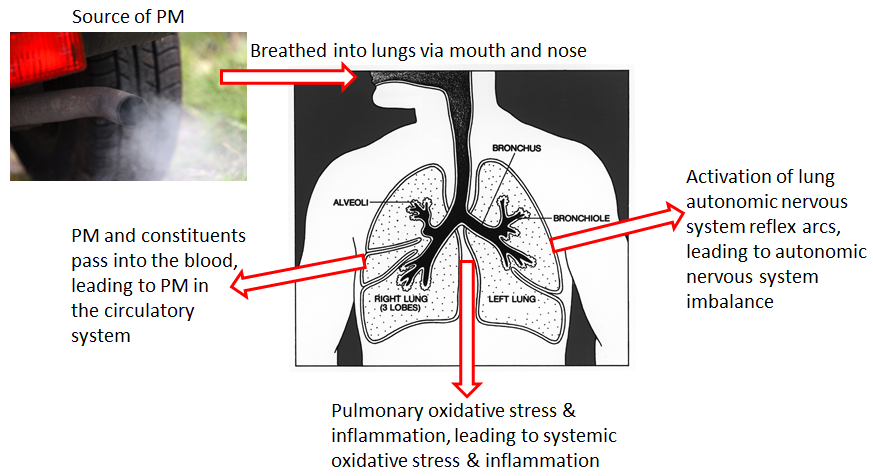
\includegraphics[scale=0.6]{biological_pathways}
\caption{The biological pathways linking PM exposure with cardio--vascular disease from \cite{Brook2010}}
\label{fig:biological_pathways}
\end{figure}

%%%%%%%%%%%%%%%%%% However I’m not going to dwell on specific pathways and biology. Suffice to say there’s something going on. Maybe it’s short term. Maybe it’s long term. Maybe it’s a combination of the both (seems most likely). But the ways of looking into it are varied.

A detailed review of the biological mechanisms underlying disease is not the scope of this thesis. Rather it is concerned with the methods of estimating levels of exposure to air pollution. The presumption of this research is that even low levels of exposure to air pollution is harmful. This is justified by studies such as the European ESCAPE project who found that long-term exposure to fine particulate pollution is associated with mortality, even at concentration ranges well below the present European annual mean limit values (\cite{Beelen2013}). The work of \cite{Brauer2002} and his group looked at the use of minimum threshold values for exposure to PM$_{2.5}$ and found that due to exposure miss-classification, population-level thresholds were apparent at lower ambient concentrations than common personal thresholds (such as the EU limit values discussed in table \ref{tab:whopmlevels} of Section \ref{subsec:urbanenvironments}).

In summary, epidemiological and toxicological studies have shown air pollution is a major environmental risk to health. By reducing air pollution levels, and exposure to air pollution, governments should be able to reduce respiratory symptoms, heart disease, and lung cancer in their population. In order to calculate the estimates of the detrimental effects on people's health, exposure and dose must be calculated as accurately as possible. That is the amount and types of air pollution that people are exposed to, and breathe in,every day of their lifetime. This can be done in many different ways, and methods are undergoing regular revision as scientists attempt to improve their accuracy. 

One of the key issues to address to further understand the links between pollutant exposure and poor health is the duration of exposure. Does long-term exposure to low levels of pollution have the same effect as short-term exposure to high levels of pollution in terms of disease prevalence or DALY? The importance of short-term versus long-term exposure on health is explored in the next section.

%%%%%%%%%%%%%%%%%%%%%%%%%%%%%%%%%%
%%% Long term v short term
%%%%%%%%%%%%%%%%%%%%%%%%%%%%%%%%%%

\subsection{Long term exposure v. short term exposure}
\label{subsec:longtermvshortterm}

%%%%%%%%%
There are few studies that compare the effects of long and short-term exposure to air pollution on a large population, at adequate spatial and temporal scales, for a range of pollutants, and with appropriate health information to enable us to determine which has the most impact on health.

%The approach that investigators have used when attributing exposure and dose values to groups of subjects for health studies (and the limitations thereof) are discussed more in sections \ref{sec:staticexposurehealth} and \ref{sec:dynamicexposurehealth}, and indeed form a crucial aspect of this research, however methods of exposure  aside, which of short-term or long-term exposure to air pollution is a more important contributor to poor health is not yet properly understood and is an issue that is being wrestled with by the community at present. 

This section therefore presents a selection of the short term and long term studies conducted to date, as well as the small number of studies that have attempted to reconcile the two. This is an issue that is being wrestled with by the community at present.

The most widely cited large-scale long-term exposure/health studies are on the effects of nitrogen dioxide in New Zealand \cite{Scoggins2004}, fine particles globally in the Global Burden of Disease 2010 ( \cite{Brauer2012}) and a meta-analysis review of both by \cite{Faustini2014}. 
Scoggins modelled annual average NO$_{2}$ concentrations over 3 km x 3 km grid squares in Auckland for the years 1996-1999 and linked these to mortality data for the same region provided by the Health Information Service. By doing this they were able to estimate that there was a 1.3\% increase in mortality for a 1 $\mu \text{g m}^{-3}$ rise in NO$_{2}$ annual average values.
Regional estimates of deaths and DALYs for the years 1990, 2005 and 2010 were estimated by Brauer using global estimates of long-term average ambient concentrations of fine particles (PM$_{2.5}$) and ozone at 0.1\textsuperscript{o} x 0.1\textsuperscript{o} spatial resolution for 1990 and 2005.
Thirdly, Faustini's review brought together studies that looked at NO$_{2}$ and PM$_{2.5}$ on population mortality and found that there was rise of 1.04\% and 1.05\% per years of life per 10 $\mu \text{g m}^{-3}$ for NO$_{2}$ and PM$_{2.5}$, respectively. Meta-analysis by \cite{Hoek2013} estimates an excess risk of 6\% per 10 $\mu \text{g m}^{-3}$ increase in PM$_{2.5}$ exposure (see \ref{fig:long_term_meta_analysis} below).

\begin{figure}[H]
\centering
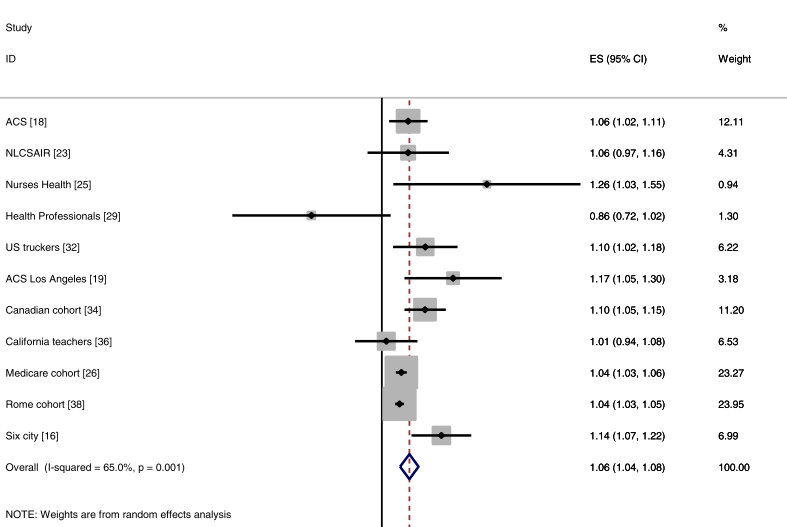
\includegraphics[scale=0.7]{long_term_meta_analysis}
\caption{Association between PM$_{2.5}$ and all-cause mortality (Relative risk per 10 $\mu \text{g m}^{-3}$) from \cite{Hoek2013}}
\label{fig:long_term_meta_analysis}
\end{figure}

As stated, links between long-term exposure and poor health seem to be fairly robust, however as long exposure time-frames that are used (typically annual average concentrations), and are combined with large spatial scales of hundreds of kilometres, it is possible that much of the detail in the results is being missed - which will be discussed more in sections \ref{sec:staticexposurehealth} and \ref{sec:dynamicexposurehealth}. Furthermore, no short-term exposure on health effect outcomes from poor air quality are considered in these 'long-term' studies, or a comparison of the importance of long-term versus short-term exposure effects.

On the flip-side, short-term epidemiological exposure health studies tend to suffer from similar issues from the perspective of someone trying to weigh-up short-term versus long-term exposure. The review by \cite{Brook2010} (briefly discussed earlier in \ref{subsec:anoverview}) concluded that short-term epidemiological time-series studies tend to find that around a 10 $\mu \text{g m}^{-3}$ increase in mean 24-hour PM$_{2.5}$ concentrations increases the risk of cardiovascular mortality by approximately 0.4\% to 1.0\% (though doesn't comment on other pollutants). But that importantly this risk is not distributed evenly across the population i.e. people with existing medical conditions or the elderly are more vulnerable to effects triggered by this short-term exposure (which comes back to the point in the previous paragraph about missing detail). Furthermore, a review of time series studies by \cite{Atkinson2014}, looking at relationships between PM$_{2.5}$, daily mortality and hospital admissions found similar percentage increases to Brook. A 10 $\mu \text{g m}^{-3}$ in PM$_{2.5}$ was associated with a 1.04\% increase in mortality. However a comparison in the same datasets with long-term exposure is not available.

Two recent studies that have sought to answer the question of short-term versus long-term exposure, or at least explore it, are those by \cite{Kloog2013} and \cite{Beverland2012a}. Kloog et al. geo-coded all deaths in Massachusetts (USA) between the years 2000-2008, modelled short-term and then long-term PM$_{2.5}$ concentrations for the area of their data-set, and then used time-series analysis to try and examine the relationships. They found for short-term relationships (day of death, and three days prior) that every 10 $\mu \text{g m}^{-3}$ in PM$_{2.5}$ there was a 2.8\% increase in PM mortality. Then for long-term exposure they found that for every 10 $\mu \text{g m}^{-3}$ increase in PM$_{2.5}$ the odds of death occurring rose to an odds-ratio of 1.6 (which simplistically equates to around a 60\% increase). Leading them to conclude that the effects of long-term air quality appear much more pronounced than short-term. Contention remains whether their definition of short-term is the most appropriate. Since the investigators only looked at PM$_{2.5}$, it might be that the effects of PM$_{2.5}$ are more pronounced in the longer--term, but NO$_{x}$ may have the opposite relationship. More data collection and analysis is needed.

\cite{Beverland2012a} take a similar approach to Kloog et al. by retrospectively using mortality data from the 'Renfrew--Paisley' and 'Collaborative' cohort studies which began in the 1970s in Glasgow (Scotland), linked to black-smoke data (the only pollutant routinely measured at the time). They too considered short-term to be three days lag, and found that there were short-term exposure-mortality associations greater than those found in the general population, indeed rises in black smoke levels were affecting mortality. Furthermore, there were also long-term mortality associations, which were more strongly associated than the short-term associations. They conclude, similarly to Kloog et al., that long-term associations have more impact than short-term. As this study was carried out retrospectively the collection of data and population definitions were not ideal. In particular, the way that the black smoke exposure was estimated using monitoring stations for short term, but modelled for long-term, introduces uncertainty. Also for comparing their associations, they used the general population for short-term and the cohort for long-term, therefore differences in these groups could cause bias in their results.

COMEAP published a report in 2010 titled \textit{'The Mortality Effects of Long-Term Exposure to Particulate Air Pollution in the United Kingdom'}. From reviewing evidence of published studies they too concluded that long-term exposure was a more important factor in contributing to mortality than short-term exposure (\cite{CommitteeontheMedicalEffectsofAirPollution2010}). Finally, bringing together many data-sets and conclusions from other studies, \cite{Stieb2002} produced a number of forest plots for different pollutants demonstrating the effect of short-term exposure. The NO$_{x}$ plot is shown in figure \ref{fig:short_term_no2_meta} which shows a consistent finding of an increase in mortality as NO$_{2}$ increases.

\begin{figure}[H]
\centering
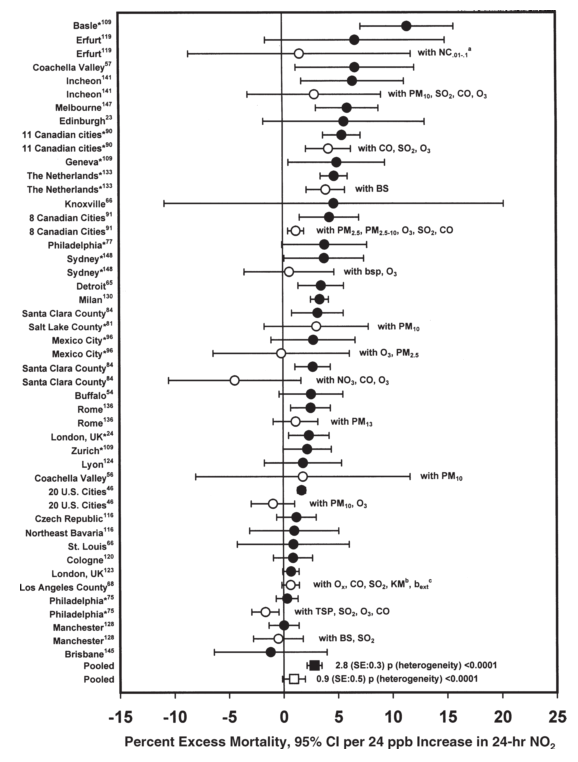
\includegraphics[scale=0.8]{short_term_no2_meta}
\caption{ Percent excess mortality from \cite{Stieb2002}}
\label{fig:short_term_no2_meta}
\end{figure}

To summarise, the research that has been conducted so far, with the data available, suggests that the effects of long-term pollution are a more important determinant of poor health than that of short-term exposure. However the studies are limited and lack detail sometimes in areas which potentially alter their conclusions. Kloog et al. and COMEAP looked at PM$_{2.5}$ (though perhaps this is sensible given the discussion in Section \ref{subsec:anoverview}), and Beverland et al. only considered black smoke. There were limitations of spatial and temporal resolution of the pollution data and subsequent linkage in the three of the studies. Often large data-sets cannot consider all important details. Definitions of how long 'long-term' and how short 'short-term' are could also be an influence on conclusions drawn. Short-term is taken to be around 3 days exposure, but this could be missing hyper-short term exposure, such as a subject spending an hour cycling down a busy road and perhaps triggering hospital admission for breathing difficulties. With better air quality data and more in-depth better information on where people spend their time (and therefore are exposed) it might be possible to overcome these issues, however the data to do this does not presently exist for epidemiologists to use.

It is important to consider both the rapid effects of air pollution exposure e.g. pathways without hours of exposure \textbf{and} the chronic effects of sustained exposure (\cite{Brook2010}).

It seems that short-term, hyper-short-term and long-term exposure are all important in understanding the health effects of air pollution. Thus studies that are able to consider large population exposures (but with information on individuals available), and on these varying time--scales are required. This issue of improving linkage between air quality and exposure has evolved over time. The next section reviews the various methods that have been used in the past to link air quality and exposure time -- what I term 'static exposure studies'. Studies that make use of various different metrics for air quality, but do not take into account the movement of people. Dynamic exposure studies are then described -- those that take this movement and other factors into account.\hfill

%This has just come out about short-term and irregular heart-beats: \url{http://www.theguardian.com/environment/2014/jun/05/air-pollution-linked-to-irregular-heart-beat-study-finds?CMP=twt_fd}

%Short-term health effects in the 'Oxford Street' study by \cite{McCreanor2007}.
\newpage
%%%%%%%%%%%%%%%%%%%%%%%%%%%%%%%%%%%
%%% Static exposure studies
%%%%%%%%%%%%%%%%%%%%%%%%%%%%%%%%%%%

\section{Static exposure \& health studies}
\label{sec:staticexposurehealth}

The methods of estimating individual and population level exposure to air pollutants (and from this data the impact on health) has evolved over time; better data has become available, computer modelling has become more complex (facilitated by more powerful computers), and more accurate methods have been employed. This section of this transfer report takes an overview of the methods of exposure assessment that I term static exposure studies. That is, the subjects to which the air pollution is being attributed do not move between environments and their exposure is calculated at their residential address. In addition the temporal and spatial granularity of the air quality data is often, in my opinion, of low or insufficient quality.\hfill

I split this into categories as follows:

\begin{itemize}
\item Large area exposure
\item Monitoring stations
\item Proximity to roads
\item Dispersion modelling
\item Land-use regression
\end{itemize}

Due to a large literature base, these sections draw on key texts for each section as examples of the approach being described. By considering the issues and problems with these studies, my proposal is that they over-simplify exposure in different ways, and justify the use of dynamic exposure models (which are explained and then thoroughly reviewed in Section \ref{sec:dynamicexposurehealth}).\hfill

%%%%%%%%%%%%%%%%%%%%%%%%%%%%%%%%%%%
%%% Large area exposure
%%%%%%%%%%%%%%%%%%%%%%%%%%%%%%%%%%%

\subsection{Large area exposure (Cities, countries etc.)}
\label{subsec:largearea}

Large area exposure studies are studies which, as the title suggests, attribute exposure to subjects over a large spatial area. This might be at the level of a city, a county or even continent. The well known Global Burden of Disease studies (discussed briefly in \ref{subsec:longtermvshortterm}) are classic examples of this approach. For the global burden of PM$_{2.5}$ (chosen due to it's strong links in the literature with poor health) in 1990 and 2005 an annual average layer of air pollution was modelled for the entire world at 0.1\textsuperscript{o} x 0.1\textsuperscript{o} spatial resolution (shown in figure \ref{fig:globalburdenpm25}).\hfill

\begin{figure}[H]
\centering
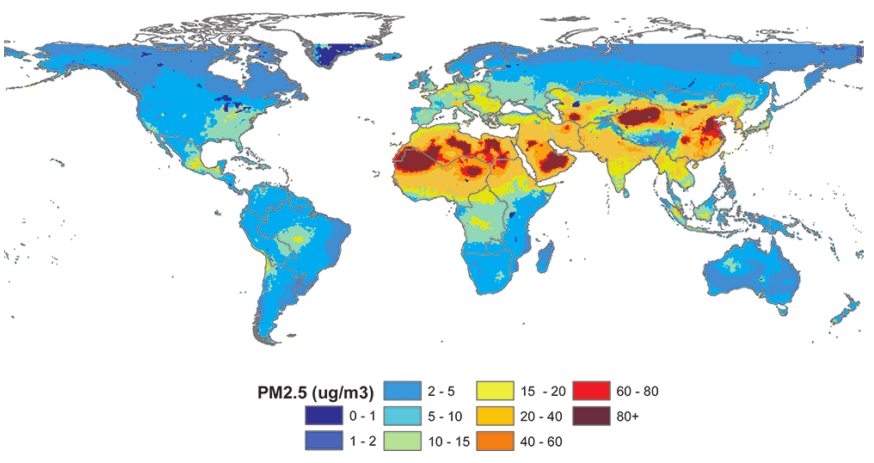
\includegraphics[scale=0.6]{global_burden_pm25}
\caption{Estimated 2005 annual average PM$_{2.5}$ concentrations (ug/m\textsuperscript{3})}
\label{fig:globalburdenpm25}
\end{figure}

To generate this worldwide layer of PM$_{2.5}$ satellite derived observations of Aerosol Optical Depth (AOD) were used (\cite{Brauer2012}). This is not a particularly common approach for exposure assessment as using satellite data for pollutant estimation and exposure as a method is still being refined, and the spatial resolution is low, however it was used in this case due to it's ability to generate data for such a large area.

The resulting health conclusions arrived at are discussed in Section \ref{subsec:longtermvshortterm}, however there are acknowledged limitations with the methods employed. Firstly, ambient concentrations are assigned to the entire population of the grid cells i.e. no micro-environmental modelling is undertaken to allow for the time that people spend indoors, or indeed in any other environment. Secondly, modelling at 0.1\textsuperscript{o} x 0.1\textsuperscript{o} resolution means much of the spatial variation in concentrations is lost, or perhaps it's better to say it's not adequately modelled in the first place. To elucidate further, we know from Section \ref{subsec:urbanenvironments} that people are concentrated in urban environments rather than distributed evenly across countries and continents, and that within these environments levels of pollution are higher than outside of them, primarily due to emissions from combustion engines (Section \ref{subsec:trafficpollution}). Taking London as an example, the city is approximately 50 km wide, yet a degree of longitude is approximately 113 km wide, meaning that (in this oversimplification example) the exposure attributed to someone living in the middle of the Kent downs where are much fewer sources of PM$_{2.5}$ is the same as someone living in the centre of London, where the sources of PM$_{2.5}$ are more frequent. The authors argue that as the population data is of a similar scale this does not matter so much, however by not being able to take account of these urban environments, or at least not at an adequate scale, exposure may be incorrectly attributed. Though to what degree it is hard to know. Thirdly, the lack of temporal resolution to the air quality layer is a problem. As was briefly explored in the sections on traffic-generated pollution (\ref{subsec:trafficpollution}) and metereology (\ref{subsec:meteorology}), air quality varies by hour, week, days, months, seasons etc. Generating annual average concentrations loses this detail and simply calculates averages for the whole year.

Studies of similar scales include \cite{Silva2013} who combined 14 atmospheric chemistry and meteorological models to attribute annual average PM$_{2.5}$ exposure to the worlds population on a scale of 0.5\textsuperscript{o} by 0.5\textsuperscript{o} degrees resolution, and \cite{Boldo2011} who modelled PM$_{2.5}$ at a resolution of 18 km by 18 km (figure \ref{fig:gspain_pm25_grid}) to cover the country of Spain (both approaches then used concentration-response functions to estimate mortality).

\begin{figure}[H]
\centering
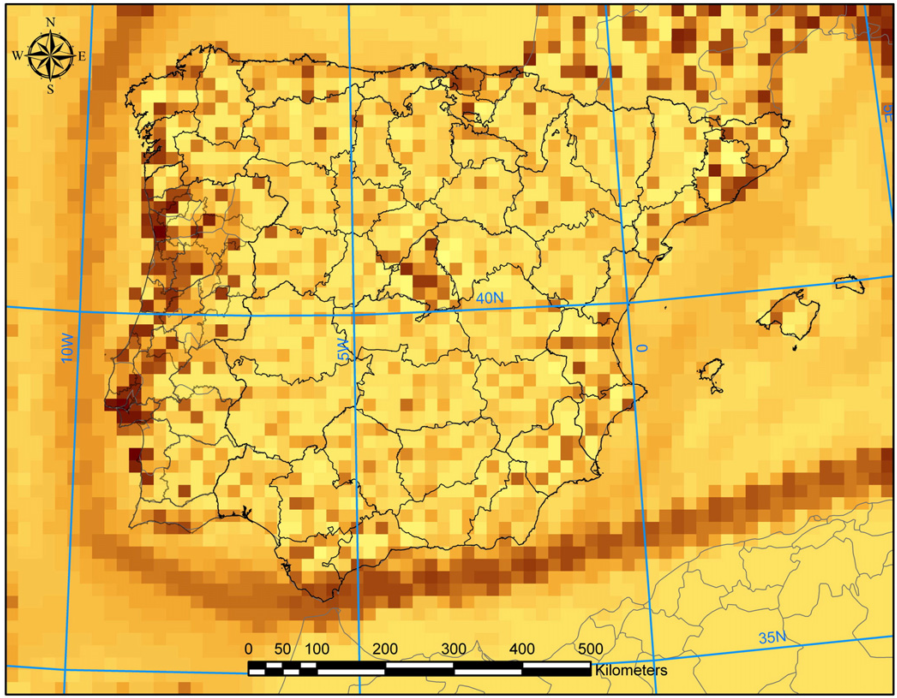
\includegraphics[scale=0.6]{spain_pm25_grid}
\caption{Grid squares used for PM$_{2.5}$ exposure from \cite{Boldo2011}}
\label{fig:gspain_pm25_grid}
\end{figure}

It should be stated at this point, that the criticism levelled at these papers is symptomatic of many studies discussed in the next sections of this report. However doing so is often a little unfair. The researchers were in most cases doing the best work that technology, available data, or indeed time or known methods allowed them to do. As we move into reviewing further literature in Section \ref{sec:dynamicexposurehealth} (Dynamic Exposure \& Health), my premis is that methods can now be improved beyond this position.\hfill

%%%%%%%%%%%%%%%%%%%%%%%%%%%%%%%%%%
%%% Monitoring stations
%%%%%%%%%%%%%%%%%%%%%%%%%%%%%%%%%%

\subsection{Monitoring stations}
\label{subsec:monitoringstation}

%% What is a monitoring station
The term 'air quality monitoring station' or simply 'monitoring station', within the context of this field of research, typically refers to a static cabin or large metal box which houses a number of instruments that measure various air pollutants and meteorological conditions at specific time intervals. A typical station is shown in Figure \ref{fig:monitoring_station}.\hfill

\begin{figure}[H]
\centering
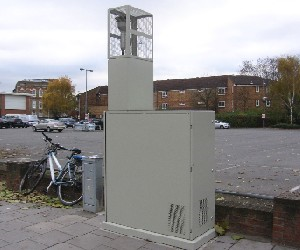
\includegraphics[scale=1.3]{monitoring_station}
\caption{A typical monitoring station (image taken from \url{www.londonair.org.uk})}
\label{fig:monitoring_station}
\end{figure}
%% Often used for regulatory purposes. Sometimes statutory.

In the UK monitoring stations were first set-up after the introduction of the Clean Air Act in 1956 but the numbers of stations, locations, the accuracy, time resolution and numbers of pollutants that are monitored has changed incrementally since then. The last change in organisation of the sites came in 1998, when the then Department of Environment established the 'Automatic Urban and Rural Network' (AURN), bringing together many sub-networks to form the most comprehensive automatic national monitoring network in the country, made up of 127 sites (\cite{DEFRA2011a}). The data collected from the sites is used for policy and legislative purposes, including reporting to the European Union, however as the data are routinely and automatically collected over long time periods the outputs have been a popular data-set for researchers too. \cite{Mayer1999} presents a good example of the temporal variability of data that can be collected such as NO, NO2, O3 and NOx at an urban air quality station in Stuttgart, Germany (and then subsequently linked to populations for estimating exposure).\hfill

One of the most highly cited research articles where data of this nature was used is in the paper '\textit{An association between air pollution and mortality in six US cities}' by \cite{Dockery1993}. In this study air pollution exposure was linked to 8111 adults over six cities in the U.S. from six monitoring sites (one in each city) in the form of annual average concentrations. Each station measured PM$_{2.5}$ and PM$_{10}$ (PM$_{15}$ before 1984). After adjusting for smoking and other risk factors, significant associations between air pollution and mortality were found. Studies that also used monitoring stations in a similar way include \cite{Atkinson2010} who did a time-series analysis of London hospital admissions using data from a background monitoring site (PM$_{10}$, PM$_{2.5}$, PM$_{10-2.5}$) and found associations between various pollutants and health outcomes outcomes such as daily mortality (particular for cardiovascular), and then \cite{Samoli2005} who as part of the APHEA Multicity Project took monitoring site data for 22 European cities and found links with mortality from the air quality data of these stations.\hfill

The main question with this type of approach however is that of temporal and spatial variability and resolution - can the data from a monitoring site be an appropriate measure of exposure for someone who, in many examples, may live miles from the monitoring site. Certainly the studies that have tried to address whether this is appropriate or not have found poor correlation between the two. \cite{Cyrys2008} found that '\textit{the use of a single monitoring station in long-term epidemiological studies must be insufficient to attribute accurate exposure levels of PNC to all study subjects}' i.e. it might work for some people but not for all. Although it's worth noting here that they believe that the monitoring stations do an accurate job of reflecting temporal variability, particularly for ultra-fine particles. Just not the spatial variability. \cite{Goldstein197747} broadly agree, they found in New York that '\textit{the procedure of using one aerometric station to represent the daily fluctuations of air pollution throughout the large metropolitan area of New York City risks the use of an unreliable or invalid measure of the short term variation in air pollution'}. So their message is slightly different, in that their research did not assesses how valid it would be as a measure of long-term variation, but they did conclude it is poor for short-term (whether long-term or short-term is more important a measure was discussed in Section \ref{subsec:longtermvshortterm}).\hfill

Whether this mis-classification of exposure to pollutants varies between pollutants and height from the ground was considered by \cite{Restrepo2004} who took data from three different monitoring stations (15m above ground) and compared it to data from a van which contained similar equipment but which was parked at three different locations and with the equipment inlets at 4m above ground.The stations showed good agreement between themselves, but not with the ground-level (van) data. PM$_{2.5}$ was closest matched, for ozone the ground level concentrations were generally lower, and for NO$_{2}$ the concentrations at ground level were over twice as high as those at the monitoring stations.

To conclude, using data from monitoring stations as a proxy for estimating exposure for large populations over many kilometres does not seem to accurately reflect individuals exposure. The studies above tended to look at the correlation between a subjects residential address and the monitoring station, meaning that there is then the additional complicating factor that people do not spend all of their time at this place. Whilst the data is certainly easily obtained and the temporal resolution makes it attractive for time-series studies, the lack of spatial variability and lack of any micro-environmental modelling or understanding of where subjects actually spend their time mean that this approach is simplistic. 

%Found this paper. May want to include it. Wallace in 2000. Review of correlations between personal exposure and monitoring stations. "Correlations of personal exposure to particles wqith outdoor air measurements: a review of recent studies".

%Also may want to inclue this paper: Text from \cite{Hou2010} .... Example of still using monitoring stations in modern times, however used a more dense network in this case and interpolation/GIS..... "A comparative analysis of human exposure to PM(10) and associated health economics was also made to see the difference between 2005 and 2008. GIS technology was employed to interpolate the distribution of population and PM(10) data collected by 27 stations at a scale of 1 km x 1 km".

%%%%%%%%%%%%%%%%%%%%%%%%%%%%%%%%%%
%%% Proximity to roads
%%%%%%%%%%%%%%%%%%%%%%%%%%%%%%%%%%
\subsection{Proximity to roads}
\label{subsec:proximitytoroads}

The use of subject's address data, and then a calculation of the number of roads (and sometimes traffic density on those roads), is another proxy measure of exposure that has been used to consider exposure to air quality and links between this and poor health. One of the most highly-cited papers in this area is by \cite{Gauderman2007}  who specifically looked at whether living near to major roadways in California had an impact on lung-function growth of children between the ages of 10 and 18. In the study 3677 children were regularly monitored for 8 years and yearly lung-function tests were completed, which were then considered alongside their home address and the distance to the nearest freeway. They found that proximity to freeway traffic is associated with substantial deficits in lung function (which became less pronounced the further the child lived from the freeway). Similar studies include those by \cite{Janssen2001} and \cite{Rose2009}, although both do not go as far as to make conclusions of health outcomes, they focus on the method of exposure estimation by road density. A wider-review of studies in this area was also undertaken by \cite{HPotHEoT-RA2010} in the HEI report '\textit{Traffic-related air pollution: a critical review of the literature on emissions, exposure, and health effects}'.

The presumption of this type of study is that the air quality the subjects  are exposed to during their normal day-to-day activities is strongly correlated to the air quality at their home, and that the air quality at their home is strongly correlated with the number of freeways within certain buffer distances of their home. These studies also mostly look at annual average traffic flows or similar, and therefore seem to not take account of variation in road use and therefore pollution levels. Indeed, combining these issues only exasperates the uncertainty, for example road flows are mostly higher during the morning and evening rush-hours, when children between 10 and 18 are likely on their way to school or already at school i.e. not at home as the model presumes. They also don't consider the time a subject is not at their home, or any other microenvironment. 

%%%%%%%%%%%%%%%%%%%%%%%%%%%%%%%%%%%
%%% Dispersion modelling
%%%%%%%%%%%%%%%%%%%%%%%%%%%%%%%%%%%

\subsection{Dispersion modelling}
\label{subsec:dispersionmodelling}

To better bridge this distance between where exposure is occurring (often presumed to be the subject's household) and where the exposure is being estimated or measured (such as a monitoring site) modelling can be used to create maps or layers of varying resolution for the area that the study or subjects are based in.

Dispersion modelling is a way of simulating the movement of emissions through the atmosphere using mathematical equations with input variables such as wind speed, wind direction, air temperature and street geography (\cite{EnvironmentalProtectionAgency2008}). By doing this at different scales (country-wide, city-wide, individual streets) it is possible to create pollution maps and to then associate the pollutant values at those places with the people who live there - estimating their exposure - and possibly linking this to health effects if data is available.

% --------Now talk here about the Maroko paper as that basically is a paper which says proximity analysis is bad and that dspersion is better. Uses environmetnal justice as the outcomes.

\cite{Maroko2012}, in studying environmental justice in New York City (USA) compared the differences between using a proximity analysis technique (similar to \ref{subsec:proximitytoroads} - proximity to roads) and a dispersion model of PM$_{2.5}$. Their hypothesis was that minority populations were more likely to be located in areas of poor air quality, and that proximity analysis may under-represent this problem. Figure \ref{fig:maroko_stack_proximity} shows tax-lots within 1\slash4 mile of the point stacks upon which the initial exposure analysis (and subsequent assessment of over-representation of minorities) was completed. 

\begin{figure}[H]
\centering
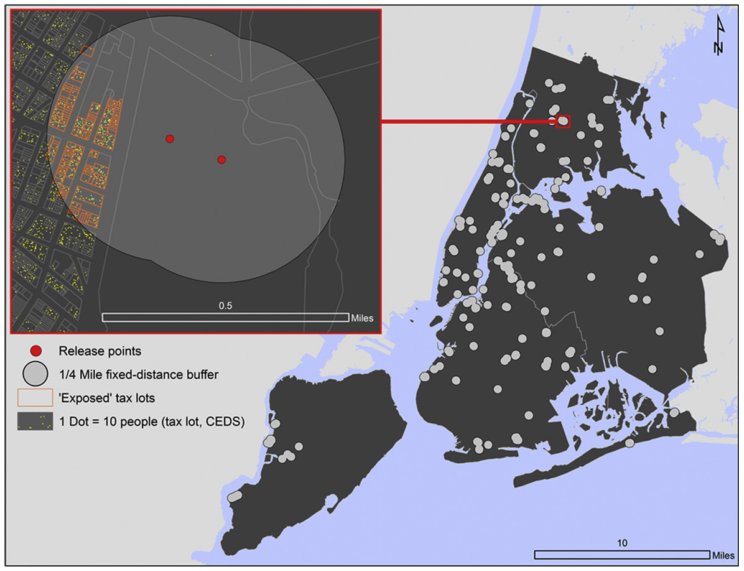
\includegraphics[scale=0.75]{maroko_stack_proximity}
\caption{Proximity analysis to PM$_{2.5}$ point sources from \cite{Maroko2012}}
\label{fig:maroko_stack_proximity}
\end{figure}

Figure \ref{fig:maroko_dispersion_map} then shows the same area, but now using dispersion modelling.

\begin{figure}[H]
\centering
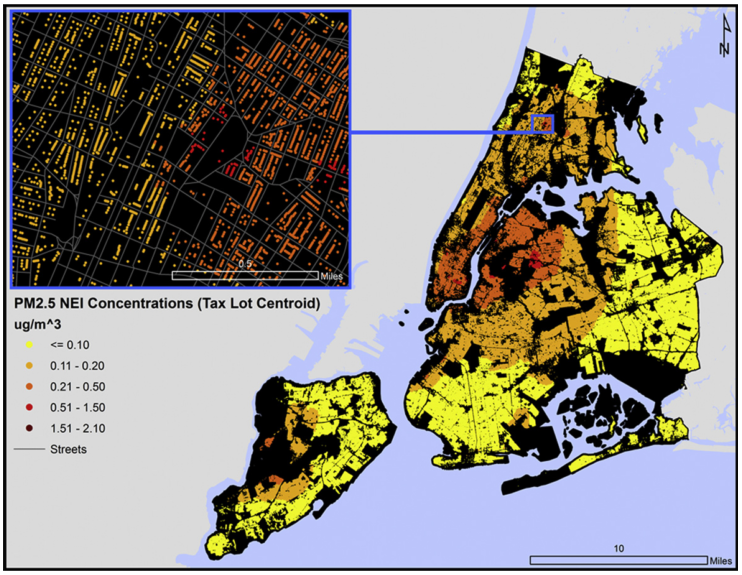
\includegraphics[scale=0.75]{maroko_dispersion_map}
\caption{PM$_{2.5}$ estimates from dispersion modelling allocated to tax--lots from \cite{Maroko2012}}
\label{fig:maroko_dispersion_map}
\end{figure}

As is clear to see, the dispersion modelling approach provides a greater degree of spatial detail and clarity. Using this second approach to exposure assessment, they were able to identify that Latino groups in the Bronx and Brooklyn were being disproportionally exposed to poor air quality than other ethnic groups, which was not evident from the proximity analysis approach. Also using a dispersion model but in London, \cite{Tonne2010} calculated the London annual average concentrations for 2001 and 2005 (pre and post the Congestion Charging Scheme (\url{http://www.tfl.gov.uk/modes/driving/congestion-charge})) for NO$_{2}$ and PM$_{10}$ on a 20m x 20m grid, and then using this aggregated the data to Ward level (shown in Figure \ref{fig:tonne_wards_dispersion}).

\begin{figure}[H]
\centering
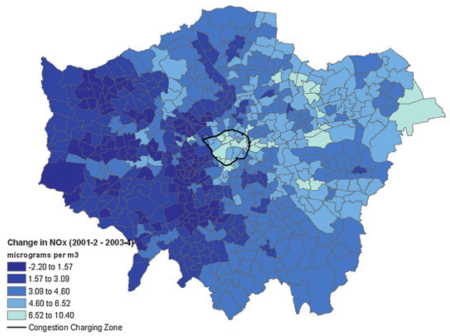
\includegraphics[scale=1]{tonne_wards_dispersion}
\caption{Map of NO$_{x}$ change at Ward level between 2001 and 2005, based on dispersion modelling (\cite{Tonne2010})}
\label{fig:tonne_wards_dispersion}
\end{figure}

The association between this change in concentration and respiratory hospital admissions was then calculated, although no conclusive relation was found.

Both of these studies (\cite{Maroko2012} and \cite{Tonne2010}) seem to be a step in the right direction for improving estimates of exposure as they provide air quality data at a higher resolution than some of the studies that were considered earlier, however there are still concerns that they mis-classify exposure by not adequately taking account of temporal variation in air quality, where the subjects are actually spending their time, and the micro-environmental aspects.

%%%%%%%%%%%%%%%%%%%%%%%%%%
%%% Land use regression
%%%%%%%%%%%%%%%%%%%%%%%%%%

\subsection{Land-use regression}
\label{subsec:landuseregression}

Land-use regression maps of air quality, and linking the concentrations from these maps to subjects for health studies, was first undertaken as part of the 'Small Area Variations In Air quality and Health' (SAVIAH) study by \cite{Briggs1997}. Land-use regression models combine monitoring of air pollution at a small number of locations, and then develop models using predictor variables normally obtained through GIS data. The model is then applied to un-sampled locations in the study area, and concentration values generated using the characteristics of the location.

A review of the use of LUR for outdoor air concentration values was published by \cite{Hoek2008} in Atmospheric Environment. They found that the models could be applied successfully to model annual mean concentrations in various geographical locations, for various pollutants including NO$_{2}$, NO$_{x}$, PM$_{2.5}$ and VOCs, and that the method was better than other geo-statistical methods such as kriging and dispersion methods. However the models were not as effective when a finer temporal scale was required or desired. \cite{Dons2013} in a study accross Flanders (Belgium) used aetholometers with a 5-minute resolution to measure black carbon at 63 locations continuously for seven days. When they compared these values to a LUR model they concluded similarly to Hoek, that existing LUR models were not ideal for considering exposure of their local population due to the lack of temporal variability. Although they did go on to develop hourly LUR models with some success (The R$^{2}$of their models varied between 0.15 and 0.79 according to the time day and the variables used as input).

In the recent paper by \cite{Pedersen2013}, which is an output from the ESCAPE (European Study of Cohorts for Air Pollution Effects) project, a LUR model was generated for 12 European countries, and then temporally adjusted using levels from nearby monitoring sites (to try to introduce temporal variability that has been lacking from this approach as noted by Hoek). Links between the concentrations at the maternal address of 74,178 women, who had singleton deliveries between 1994 and 2011, were then examined. They found that a 5 $\mu \text{g m}^{-3}$ increase in concentration of PM$_{2.5}$ during pregnancy was associated with an increased risk of low birthweight at term (adjusted odds ratio of 1.18).

To summarise, LUR models are being used for health studies, and conclusions between health outcomes and air pollution are being drawn, however there are similar problems with the exposure estimates\slash linkages as in many of the other previous static exposure estimate methods, including that there is no estimation of the amount of time that people spend away from their home and the pollutants and concentrations that they are exposed too i.e. how much time did the mothers in the ESCAPE study actually spent at their maternal address? Studies using LUR also don't tend to conduct any micro-environmental modelling of the time that subjects spend indoors or in transport, and the methods behind the temporal variability might be considered further i.e. is using a nearby monitoring stations daily variation sufficient to reflect the daily variation at the address point.

A more generic problem with using LUR models for exposure assessment is that LUR models need monitoring to be conducted in the area that the model is proposed to be used in. Setting up a dense enough network of monitors to provide accurate model results is expensive and time--consuming.

\vspace{1cm}

In the review article \textit{"Spatio-temporal epidemiology: principles and opportunities"} \cite{Meliker2011} discusses how exposure estimation is a rapidly changing field, and how GIS, computer power and 'big data' have started to overcome issues that spatio-temporal epidemiology has often struggled with (as discussed in the preceeding sections). One of the areas that is still somewhat lacking however, despite exposure assessments producing estimates of contaminants changing through time and space (e.g. temporal air pollution maps), however, is human mobility -- it is seldom incorporated. They conclude their review with the following quote, which sets the scene for the following section titled 'Dynamic exposure and health studies', those being studies that explicitly seek to take account of the movement of individuals through different environments, and their exposure in those environments:

\begin{quote}
"We expect exposure assessments to increasingly incorporate space--time dynamics in particular mobility and environmental contaminants, such that it becomes commonplace in the near future" \cite{Meliker2011}
\end{quote}
\label{chap:background}
\newpage
\section{Dynamic exposure \& health studies}
\label{sec:dynamicexposurehealth}

As we have seen from the studies reviewed thus far, effectively and accurately quantifying exposure to air pollution is fraught with problems. Exposure methods that include sufficiently large numbers of subjects often find it difficult to accurately assign exposure; as the subjects spend time in many different environments, travel between these micro-environments, and often the air quality data is of insufficient temporal or spatial quality. Then the epidemiological studies that are based upon these exposure estimations may therefore be arriving at incorrect health associations and conclusions. \cite{Brauer2002} measured personal exposure and compared it to monitoring site exposure for \gls{pm25} for 16 subjects in Canada and found that in 13 of the 16 subjects the measured ambient concentrations were under-representing exposure. Ashmore's review of literature focusing on children's exposure found that their exposure is closely related to concentrations in the home, at school, and in transport, differing significantly from adults concentrations and general outdoor concentrations such as those at monitoring sites (\cite{Ashmore2009}).

Although the links between health and air pollution are fairly clear, as discussed in section \ref{sec:healtheffects} (\nameref{sec:healtheffects}), it might be that this miss-classification error is biasing any calculated risk factors, regressions or coefficients towards the null value (no association) i.e. once exposure classification is improved the relative risks of increases in exposure to pollutants may be greater than previously thought (\cite{Armstrong1990}).

%%%%%%%%%%%%%%%%%%%%%%%%%%%%%%%%%%%%%%%%
%%%%% PERSONAL MONITORING %%%%%%%%%%%%%%
%%%%%%%%%%%%%%%%%%%%%%%%%%%%%%%%%%%%%%%%

\subsection{Personal Monitoring}
\label{sec:personal_monitoring}

To gain further insight and a more accurate estimate of individual-level exposure to pollutants, personal monitoring methods can be used. Studies that are described as personal monitoring vary in their use of equipment, and measuring of different pollutants, but generally describe studies that attach portable pollutant monitoring devices to a person or persons, who then go about their normal lives while the devices collect data. The devices normally collect data at short time intervals i.e. one minute, and are combined with location devices like a Global Positioning System (\gls{gps}). By using these devices in combination researchers are able to collect data on concentrations at the the places that the subjects are in, and see how levels vary between them. Using such equipment individual level objective direct measures of exposure can therefore be collected. These studies are often considered the "gold standard" of exposure assessment (\cite{Ashworth2013} , \cite{DeNazelle2008}).

\cite{Steinle2013} conducted a review of personal exposure studies of this type. They discussed the difference between traditional exposure assessments using fixed air quality network sites, single micro-environments, and static populations - compared to the new developments in sensor technology that have enabled researchers to directly monitor pollutants while people move through varying concentration fields and activity space. They summarised the personal exposure approach with Figure \ref{fig:traditional_personal_monitoring} which visualises the joining of location data and air quality data

\begin{figure}[H]
\centering
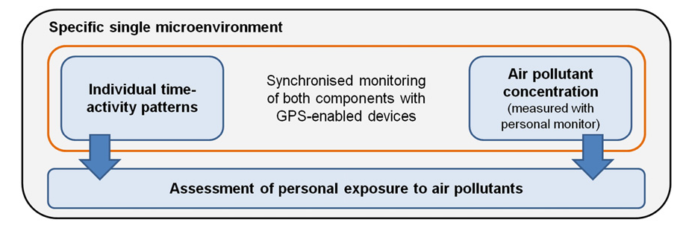
\includegraphics[scale=0.7]{traditional_personal_monitoring}
\caption{Conceptual model illustrating the traditional approach for the assessment of personal exposure to air pollution}
\label{fig:traditional_personal_monitoring}
\end{figure}

This area of air pollution exposure research has, as Steinle notes, accelerated in popularity recently due to the advancements in related technology. The devices have become cheaper, lighter and easier to collect/process data from. The ubiquitous nature of smart phones has also contributed in terms of it becoming the norm for people to carry about technology and have elements of their lives tracked. Indeed, studies such as \cite{DeNazelle2013} have used data from smartphone applications that are not designed for exposure assessment, but which offer a rich data set e.g. the application CalFit for estimating peoples movement style i.e. running, cycling, walking. A search of the terms ('personal exposure' AND 'air pollution') in PubMed, summarised by year of publication in Figure \ref{fig:personal_exposure_publications},  illustrates the increase in these studies (whilst acknowledging that there are mitigating circumstances such as the popularity of the field as a whole, and numbers of journals in this area etc.):

\begin{figure}[H]
\centering
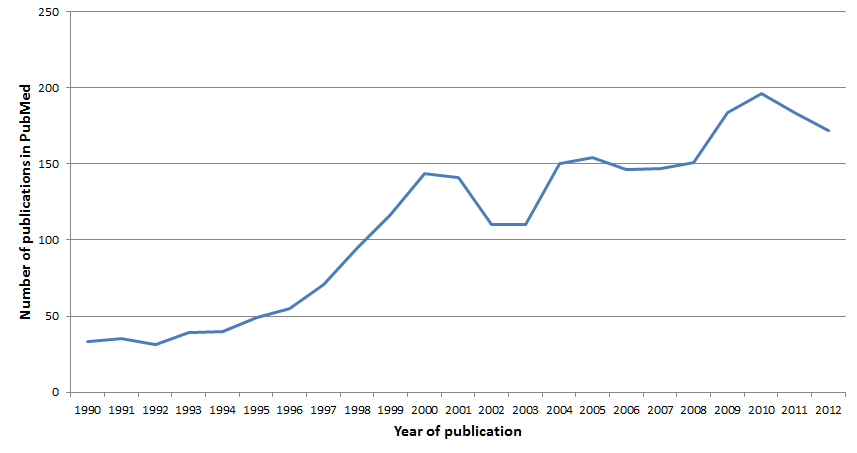
\includegraphics[scale=0.5]{personal_exposure_publications}
\caption{Numbers of publications about personal exposure to air pollution in PubMed}
\label{fig:personal_exposure_publications}
\end{figure}

\cite{Dons2011} in Belgium completed personal monitoring campaigns for 16 couples. One member of each couple was identified as a full-time worker, and one as a homemaker. Each couple's personal exposure was measured over 24 hours by them carrying a micro-aetholometer and a \gls{pda} device which contained a \gls{gps} chip for location and time-activity diary for contextual information (which was subsequently completed by the individuals). Very different patterns of exposure were observed between the couples, despite them living in the same place i.e. two individuals living in the same location would have the same exposure according to some of the approaches in the static studies section. Exposure differed by upto 30\% between couples, with exposure during transport being identified by Dons et al. as the most important factor in this discrepancy. In a similar study in Italy, \cite{Buonanno2014} conducted personal monitoring on 24 non-smoking couples and measured their exposure to ultra-fine particles using a Phillips NanoTracer (which included a \gls{gps}). In this study the couples were all male-female, the male being a full-time worker and the female being a homemaker. Given the emphasis that Dons found on transport, it was slightly surprising that this study found women to have higher exposure than men. This was attributed to the emissions from cooking stoves in the home and that the particles stay in the environment for prolonged periods. Although the two studies actually consider different metrics (black carbon compared to ultrafine particles) so the comparison is hard to make directly -- there are not many sources of black carbon in the home, but transport is a major source outside of the home. In a further study \cite{Broich2011} used a \gls{gps}, and GRIMM 1.09 monitor to measure particulate matter (in various sizes) for sixteen people over 24 hours each in Italy.

\begin{figure}[H]
\centering
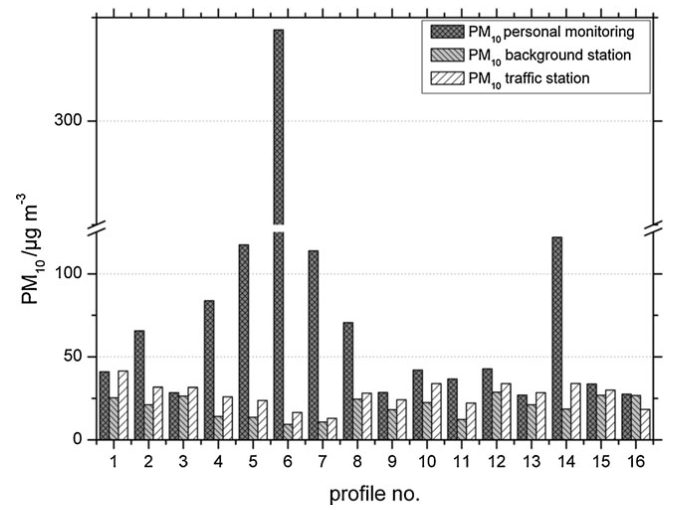
\includegraphics[scale=0.6]{broich_exposures}
\caption{Average exposure over 24 hours to \gls{pm10}, comparing personal monitoring, background monitoring stations and traffic monitoring stations}
\label{fig:broich_exposures}
\end{figure}

As can be seen in Figure \ref{fig:broich_exposures} from \cite{Broich2011}, there were large variations between the personal exposure concentrations, and concentrations at nearby monitoring sites. The averages over 24 hour between participants varied from 27 to 322 $\mu \text{g m}^{-3}$, and like Dons they found that exposure levels were heavily dependant on the travel participants undertook, and the micro-environments they spent time in. Broich argues this is why direct personal exposure monitoring is needed for accurate exposure assessments rather than proxy methods (monitoring sites or address). Although for epidemiological studies that might relate patterns from monitoring sites to patterns in incidents of poor health, this may not necessarily the case. If the personal exposure results for instance are always say 40\% than the monitoring site, then the monitoring sites would still capture the trends and might be able to relate these trends to hospital admissions. 

While these types of study are excellent at providing hyper-local and time resolved personal exposure data, they tend to struggle to provide data that is useful for considering alongside the harmful health effects of poor air quality. The studies give results for individuals or small groups of people which are not able to be used alongside health-related epidemiological data such as hospital admission records or incidences of asthma in a certain region. As \cite{Chaix2013} argues, improving measuring of exposure to environmental conditions by accounting for the movement of individuals is critical, however by using such small numbers there is a danger of over-generalisation between exposure and health. Measuring 20 school-children's exposure to \gls{pm10} for example, and then making wide-ranging assumptions about the health effects of \gls{pm10} on all school children seems overly simplistic. It might be that those 20 children are in the top 5\% of exposures and not a good representation of school children in general.

\cite{Steinle2013} argues that the trend in the area of calculating accurate exposure estimates for large populations is for the development of the personal monitoring approach, i.e. distribution of low-cost, accurate \gls{gps} devices combined with accurate low-cost unobtrusive portable air quality measurement devices. In this way the amount of data collected through this 'gold-standard' method would be adequate to allow extrapolation to large groups of people i.e. if 80\% of school children carried a monitor for 12 months, then concerns about how representative the data is would be less valid. A model of their theoretical approach is shown in \ref{fig:steinle_full_assessment}.

\begin{figure}[H]
\centering
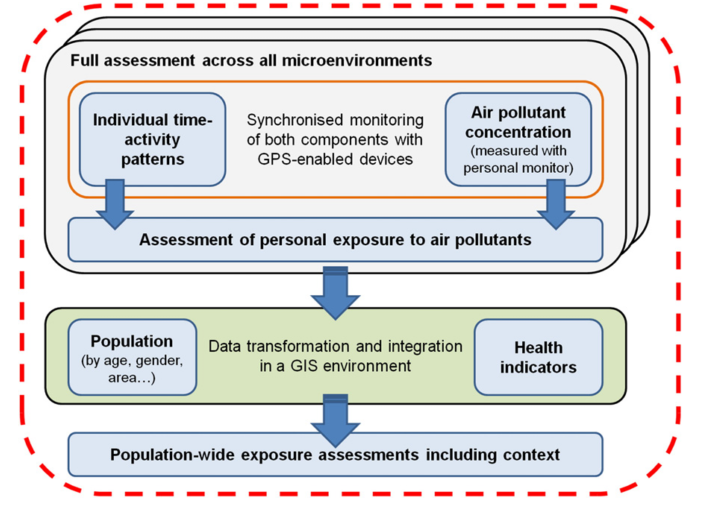
\includegraphics[scale=0.8]{steinle_full_assessment}
\caption{Conceptual model for the assessment of individual and population-wide exposure to air pollution including effects}
\label{fig:steinle_full_assessment}
\end{figure}

\cite{Minguillon2012} seemingly agree with this large-scale personal monitoring approach, or at least with the notion that personal monitoring is required to properly understand exposure. In their study on pregnant women's exposure in Barcelona in 2009 they compared measurements from the subjects household balcony, inside their house, and the data from personal monitoring equipment. They found mean concentrations for \gls{pm25} of 20 $\mu \text{g m}^{-3}$, 24 $\mu \text{g m}^{-3}$, and 27 $\mu \text{g m}^{-3}$, for outdoor, indoor, and personal samples respectively. They concluded that it was important to rely on personal exposure measurements for epidemiological studies.

Against this approach however is the practical nature of conducting these monitoring campaigns. The technology for this type of study is not yet available (as the above authors note). In addition, even if it were, the distribution of the devices and automated collection of the data on a large enough scale would seem difficult to achieve. Though this may change with the advent of smaller and lower-cost measurement technology. What personal monitoring studies do show researchers in this field is where subjects the majority of their time (indoors), and where they are exposed to the highest levels of air pollution (normally during travel). By doing so they emphasise how important these factors are in understanding the true exposure of individuals compared to current or traditional methods.

Developing a modelling approach, with a focus on the accuracy of the modelling in these environments to improve exposure estimates, seems a more practical approach to better understanding population exposure.

%%%%%%%%%%%%%%%%%%%%%%%%%%%%%%%%%%%%%%%%
%%%%%%%%%% INFILTRATION %%%%%%%%%%%%%%%%
%%%%%%%%%%%%%%%%%%%%%%%%%%%%%%%%%%%%%%%%

\subsection{Infiltration}
\label{sec:infiltration}

%% What is infiltration
Infiltration refers to the diffusion of outdoor air into the environment inside a building. The amount of outdoor air that ingresses depends on ventilation, air conditioning and on the indoor--–outdoor temperature gradient. \gls{eu} guidelines now state that buildings must be insulated to save energy, however as buildings allow less air to be exchanged with the outside environment, the indoor concentration of pollutants can increase if there are significant indoor sources. Thus increasing the air-tightness of buildings can have negative impacts on health (\cite{Gens2014}). This is offset of course by meaning that harmful outdoor-generated pollutants will not as easily be able to infiltrate into the indoor environment. The study of indoor air has steadily become an inherent part of modern exposure research (\cite{Steinle2013}). Figure \ref{fig:infiltration} below illustrates how outdoor air infiltrates buildings and mixes with indoor air (from \cite{Chen2011}).

\begin{figure}[H]
\centering
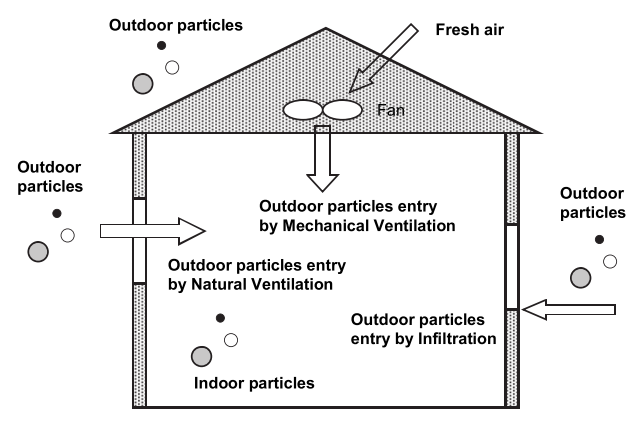
\includegraphics[scale=0.8]{infiltration}
\caption{Infiltration}
\label{fig:infiltration}
\end{figure}

Indoor pollutants have many sources such as cigarette smoke, cooking, heating and cleaning products. They can substantially change a persons exposure (compared to ambient concentrations), and characterisation of them is difficult. To consider the exposure of subjects to air pollution over days/weeks/months, indoor air is an important consideration.  A better understanding of the factors influencing infiltration and indoor sources can improve exposure assessment methods and contribute to reduced exposure miss-classification in epidemiological studies (\cite{Colbeck2010a}, \cite{MacNeill2012}). Doing so depends on the metrics that are being used for considering the health effects e.g. to better understand the effects of traffic pollution on health, indoor sources (cooking, heating) would not be  needed and the infiltration of outdoor air into the indoor environment would be key. But for a model which considered exposure to all pollutants then all sources would be needed.

%% Some studies that have looked at indoor concentrations
To try and better understand the differences between indoor and outdoor air quality, as part of a large cohort exposure study in Ontario (Canada), \cite{MacNeill2012} measured concentrations of \gls{pm25}, ultra-fine particles (\gls{ufps}), black carbon and humidity both inside properties and in the back garden of properties simultaneously for two weeks. As is common with this type of study the results were discussed in terms of indoor\slash outdoor ratios, otherwise known as I\slash O ratios. This is the concentrations inside the property, divided by the concentrations outside of the property. So if a property had a \gls{pm25} I\slash O ratio of 0.5 at 10am and the concentrations outside were 10 $\mu \text{g m}^{-3}$, then this would mean that concentrations inside the property were 5 $\mu \text{g m}^{-3}$ (10 multiplied by 0.5).

The median daily estimates found in the study ranged from 0.26 to 0.36 across seasons for \gls{pm25}, with the ranges typically related to window-opening behaviours, air conditioning, meteorological variables, home age, use of electrostatic precipitators and stand-alone air cleaners. The determinants of indoor source concentrations were related to cooking, candle use, supplemental heating, cleaning, and s of people in the home. Expanding on the last of the variables noted by MacNeill, \cite{Colbeck2010a} comments on the close relationship between indoor concentrations and human activities, stating that humans are responsible for their own 'personal cloud' i.e. exposure to airborne particles resulting from their own activity.

\cite{Challoner2014} looked at \gls{pm25} and \gls{no2} concentrations in ten different city centre buildings in Dublin. They found \gls{pm25} I/O ratios close to 1 (similar to outside air) for the ten commercial buildings, however after studying the temporal variation in these levels they suggested that indoor sources and/or re-suspension of \gls{pm25} seemed to have a more significant impact compared to variations in outside air quality. \cite{Kearney2014} measured\gls{pm} continuously for seven consecutive days in 74 Edmonton (Canada) homes in 2010. Simultaneous measurements of outdoor (near-home) and ambient (at a central site) concentrations were also measured. As with the studies above, they found considerable variability ranging from 0.10 to 0.92 in winter and from 0.31 to 0.99 in summer.

Given the number of variables that seem to contribute to variations in indoor air quality, making broad-sweeping assumptions to create inputs to epidemiological models seems difficult. However \gls{who} calculated in 2005 that people spend 89\% of their time indoors, \cite{Lai2004a} found a figure of (89.5\%) from their research, and \cite{Schweizer2007} found similar - 20.66 hours (86\%). Efforts to better quantify this exposure relationship and create as accurate a picture of exposure are therefore needed. The variability in I/O ratios within and between homes may cause substantial exposure miss-classification compared to only using ambient measurements (\cite{Kearney2014}).

A dynamic exposure model i.e. one that is going to take account of different micro-environments where people spend their time, needs to attempt to model concentrations indoors. People spend such a large percentage of their time indoors that this environment needs 'adjustments' from ambient concentrations. The following paragraphs therefore consider a few recent studies that have attempted this.

MESA-Air stands for the "Multi-Ethnic Study of Atherosclerosis and Air Pollution" and was a large research project based in Washington State (\gls{usa}). The project was designed to examine the relationship between air pollution exposures and the progression of cardiovascular disease (\cite{Allen2012}). To do this the researchers needed to quantify exposure to indoor air, and so they aimed to develop models to predict I/O ratios for around 6,000 homes. They did this by collecting 526 two-week, paired indoor–-outdoor \gls{pm25} filter samples from a subset of homes in their study. Taking account of specific weather and seasonal variables, as well as using information from questionnaires, they made a regression model which predicts I/O ratios (mean of 0.62, SD of  0.21) using easily obtained variables. This is an important study in the cross--over area of air pollution exposure assessment, indoor--outdoor concentrations and epidemiology as it was the first study with a large number of subjects to incorporate variation in residential exposure into exposure assessment. The effect that this new information made to epidemiological study of the prospective cohort is not published at the time of writing.

\cite{Hussein2014} took a similar approach with their exposure model, however they also considered dose (Figure \ref{fig:husseiniomodel}). Their model calculates exposure by considering infiltration into the indoor environment, indoor sources, building types, building sizes and the time-activity pattern of the individual. A mass-balance model is used for the indoor exposure which not only models infiltration but the indoor sources.

\begin{figure}[H]
\centering
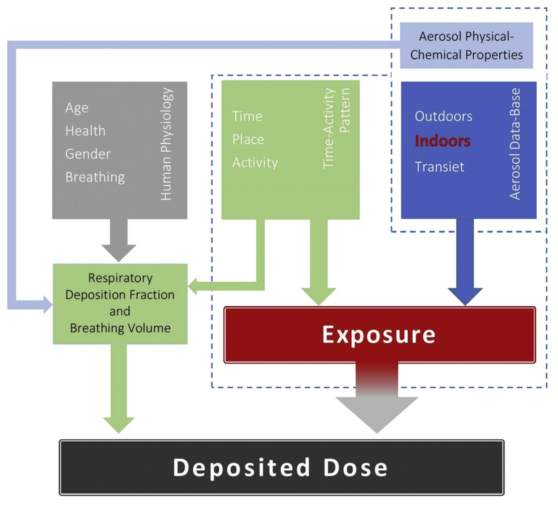
\includegraphics[scale=0.7]{hussein_io_model}
\caption{Exposure model incorporating indoor exposure}
\label{fig:husseiniomodel}
\end{figure}

They illustrate the use of the model by calculating exposure and dose for 24 hours for a test individual, showing the inputs needed for the various model parameters. The advantage of this approach is that it starts to show a way for indoor exposure to be properly included in an exposure assessment model, however as the authors acknowledge the detail and amount of data required for input to the model (i.e. volumes of buildings, detail of indoor sources, time activity patterns) is not yet available on a large enough scale and robust enough, to expand this approach to large numbers of subjects. Lacking exposure modelling of the journeys between the environments would also seem to be necessary for this model to give a more holistic picture of exposure. However the inclusion of the calculation of dose in such a dynamic exposure model is clearly a positive step. Dose being a quantification of the amount of pollutant(s) that the subject actually breathes in and makes its way to the airways and lungs of the subject as per the discussion and diagram of \cite{Brook2010} in Section \ref{subsec:anoverview}.

\cite{Johnson2012} also developed a dynamic exposure model that considered pollutant levels in indoor micro-environments, specifically focusing on \gls{no2}. They had 60 school-children (ages 12--13) wear personal monitors for two days and while doing so keep a detailed log of their activity, location, and the activity of others around them that might generate pollutants e.g. their parents cooking or smoking at home. Using the time-activity patterns, modelled outdoor concentrations and I/O ratios from literature (e.g. 2 for cars/buses, 0.5 for school) they calculated exposure for the set of children and compared it to their monitored data. The results of this micro-environmental exposure model agreed well with the personal exposure measured by the children, however a great deal of contextual information was required to come to such close agreement and it is hard to see how a model of this type could be applied to a much larger cohort of subjects without the same level of detail available. Given this the transfer-ability of the study to other subjects and areas is not useful as a tool in and of itself, but it does show that good agreement can be obtained between modelling and monitoring of personal exposure given sufficient data. An additional problem with using this approach elsewhere is that the air quality data was based on a land-use regression model, which as was discussed in Section \ref{subsec:landuseregression} (\nameref{subsec:landuseregression}), requires extensive monitoring to be accurate and often lacks temporal variation.

As discussed earlier in this research, the health effects of exposure to air pollution are not yet fully understood. Studies have tended to assign exposure based on outdoor concentrations at the subjects residence using long term average concentrations or on monitoring stations concentrations for studies of short-term exposure. Given this it is no surprise that the negative effects of poor indoor air quality on a populations health are similarly not yet understood (although the approaches discussed in the preceding paragraphs are contributing to a better of understanding of overall exposure i.e. they are starting to contribute to understanding and quantifying exposure indoors, while other studies that quantify exposure in other environments are completing the picture).

\cite{Gens2014} is one of very few studies that have attempted to consider how indoor air is affecting health, specifically looking at the increase in air-tightness of modern EU buildings. The assessment was based on modelling exposure to fine particles originating from both outdoor and indoor air, including environmental tobacco smoke. Exposure response relationships were derived and the results showed an increase of adverse health effects in all considered countries (ranging for health effects from 0.4\% in Czech Republic to 11.8\% in Greece for 100\% insulated buildings) due to an accumulation of particles indoors. Unsurprisingly considering only the effects of outdoor air led to a decrease of adverse health effects.  Although the conclusions drawn for this response relationship seem in doubt as the odds-ratios have been applied to the combination of indoor and outdoor air, when they are only designed and suitable to be used for outdoor air.

\cite{Chen2011} conducted a review of modelling approaches on the relationship between indoor and outdoor particles and summarised that I/O ratios vary considerably due to the difference in size-dependent indoor particle emission rates, the geometry of the cracks in building envelopes, and the air exchange rates. Concluding that due to this it is difficult to draw uniform conclusions on I/O ratios, as they vary so much between building types.

The studies discussed in this section show that indoor air varies considerably from outdoor air, and that research is ongoing as to how to effectively model this as part of a holistic exposure model that also incorporates other environments such as different transport modes. Research so far has identified that indoor air quality is effected by outdoor concentrations, the number and activity of people inside the building (particularly apparent for particulates), the ventilation systems (or lack of), indoor sources, meteorology and the air-tightness of the building.

%%%%%%%%%%%%%%%%%%%%%%%%%%%%%%%%%%%%%%%%
%%%%%%%%%%%%% TRANSPORT %%%%%%%%%%%%%%%%
%%%%%%%%%%%%%%%%%%%%%%%%%%%%%%%%%%%%%%%%


\subsection{Transport}
\label{sec:transport}

As briefly discussed in Section \ref{subsubsec:invehicle} ('\nameref{subsubsec:invehicle}'), air quality when in transport can differ greatly from ambient concentrations. Table \ref{tab:adams_transport_means} (also from Section \ref{subsubsec:invehicle}) showed measurements in different transport modes which were different (mostly higher) than that of the ambient concentrations. A review of pollutant concentrations in different transport modes by \cite{Karanasiou2014} provides an excellent resource for considering the breadth of the differences between in-transport air and ambient air. Reflecting transport exposure as part of a persons total exposure is important as it is thought that individuals gain a significant contribution of their daily exposure during travel, despite the small percentage of time  that is typically spent doing so. For black carbon exposure \cite{Dons2011} found subjects spent 6-8\% of  their day in transport, where they accumulated 21\% of their exposure. Failing to account for these important exposure events contributes to exposure miss-classification. 

As can be seen from the data compiled by the Office for National Statistics (\cite{OfficeforNationalStatistics2010}) in Figure \ref{fig:transportprofiles}, the three most popular modes of transport in England and Wales over the last half a century have been car and van, followed by bus and coach, and finally rail. 

\begin{figure}[H]
\centering
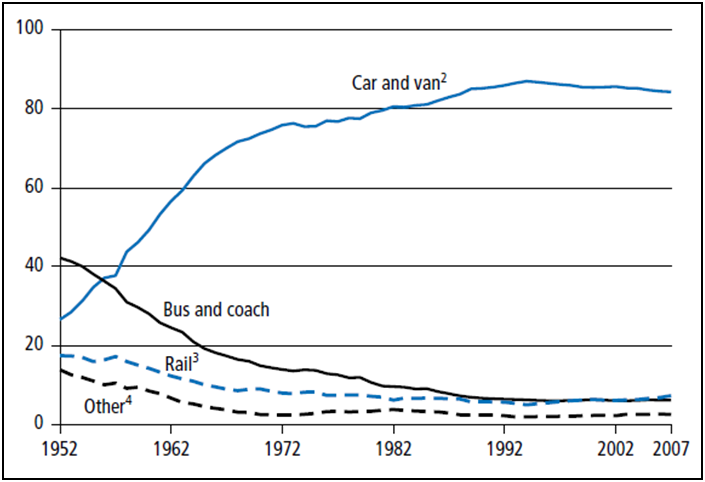
\includegraphics[scale=1]{transport_profiles}
\caption{Transport profiling from Office for National Statistics (\gls{ons}) census data between 1952 and 2007}
\label{fig:transportprofiles}
\end{figure}

Studies which have sought to measure and understand exposure in these transport modes are now discussed, with the addition of cycling. Cyclists are included as a special case due to their increased inhalation rates and proximity to road traffic which may significantly increases their exposure and dose of poor air quality.

%% A paper here that I've been given after this was done that might want to include. It's about exposure in transport.
%% http://www.arb.ca.gov/research/seminars/zhu/zhu.pdf

%%%%%%%%%%%%%%%%%%%%%%%%%%%%%%%%%%%%%%%%
%%%%%%%%%%% BUS AND COACH %%%%%%%%%%%%%%
%%%%%%%%%%%%%%%%%%%%%%%%%%%%%%%%%%%%%%%%

\subsubsection{Bus and Coach travel}
\label{sec:bus_and_coach}

The review by \cite{Karanasiou2014} found that pollutant concentrations inside buses and coaches vary greatly by country, likely reflecting the variation in weather conditions, vehicle types, ambient concentrations, and fuel sources of the vehicle/surrounding fleet. In one study concentrations in the Netherlands were found to be higher in diesel vehicles than on the same routes with electric fuelled buses, suggesting that the own vehicles exhaust impacts on the exposure inside the vehicle (vehicle 'self pollution'). Though this could also be reflective of the permeability of the vehicle or the number of times the doors were opened or closed, allowing ambient concentrations to ingress. When compared to ambient concentrations, a Paris study found an I/O ratio of 1.3, and in the Netherlands a similar ratio of 1.43. Typical \gls{pm25} concentrations inside the vehicle across the eleven studies reviewed were in the range 35 -- 69 $\mu \text{g m}^{-3}$.

A study not covered in the review is by \cite{Song2009} in York, U.K. Measurements were made simultaneously by placing an optical particle monitor in the middle of a bus in York over a period of three days in May 2007, and comparing the data recorded to measurements from an identical monitor on the bonnet of a car which followed the bus (\cite{Song2009}). Measurements were completed during the morning and evening rush hours over 24 hours. Figure \ref{fig:bus_ratios} shows how the relationship between out-bus and in-bus concentrations was positively linear, with a higher gradient as particle size increases (the column labelled 'Dependent variable' is the size fraction of \gls{pm}). Also having the windows closed on the bus actually led to increased concentrations compared with having the windows open, suggested to be due to re-suspension by passenger activity. 

\begin{figure}[H]
\centering
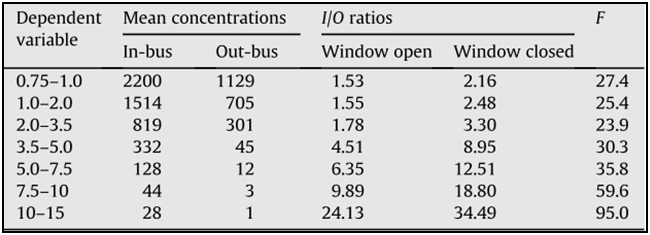
\includegraphics[scale=1.2]{bus_ratios}
\caption{Comparison of mean in-bus and out-bus particle concentrations}
\label{fig:bus_ratios}
\end{figure}

I/O ratios for PM in the size range of 0.75 to 2.0 are 1.53 and 1.55 for when the windows are open, and 2.16 and 2.48 for when the windows are closed. There are many other factors which complicate drawing conclusions between studies, but it is interesting to note how closely the former of these ratios agree with the studies in Paris and the Netherlands for similar PM fractions discussed at the start of this section. 

Using data from this study, the \cite{Song2009} paper concludes by compiling a model for estimating the indoor/outdoor ratio of different PM fractions. The model showed broad agreement with measured particle concentrations inside buses and demonstrated that re-suspension by passenger activities and deposition to the surface of the passengers had significant effects on the concentrations.

The health implications of bus and coach exposure is not discussed by the Karanasiou review or the Song paper as a separate issue or metric. Being able to include exposure by this transport mode in a large-scale exposure assessment exercise is required for exposure mis-classification to be reduced. Though is further complicated, as in many of the sections of this report, by the composition of particles i.e. particles from different sources have more or less harmful effects on health.

%%%%%%%%%%%%%%%%%%%%%%%%%%%%%%%%%%%%%%%%
%%%%%%%%%%%%% CAR TRAVEL %%%%%%%%%%%%%%%
%%%%%%%%%%%%%%%%%%%%%%%%%%%%%%%%%%%%%%%%

\subsubsection{Car travel}
\label{sec:car}

Studies on exposure while travelling inside cars are more frequent than those of other transport modes. From reviewing studies of car exposure \cite{Karanasiou2014} found that typical European particulate matter concentrations inside passenger cars were in the range of 36–-76 $\mu \text{g m}^{-3}$ for \gls{pm10} and 22-–85 $\mu \text{g m}^{-3}$ for \gls{pm25}. Whether the car itself was powered by diesel or gasoline was found in most studies to make little difference to particulate matter, particle number counts and black carbon. However \cite{Jalava2012} found that pollutant concentrations inside the car depended highly on the type of fuel used.

A separate review by \cite{Nasir2009} found that exposure to particulate matter in the car micro-environment is largely dependent on traffic congestion, road network layout, vehicle design/condition and ambient concentrations.

\cite{Dons2013} studied slightly different parameters, or ways of considering the parameters, of black carbon exposure in vehicles in Figure \ref{fig:road_type_exposure}. It was noted that in urban areas concentrations inside vehicles are higher compared to exposure in more rural areas; with the same holding true for highways versus local roads for motorists -- suggesting that the surrounding fleet and traffic speeds affect in-vehicle concentrations.

\begin{figure}[H]
\centering
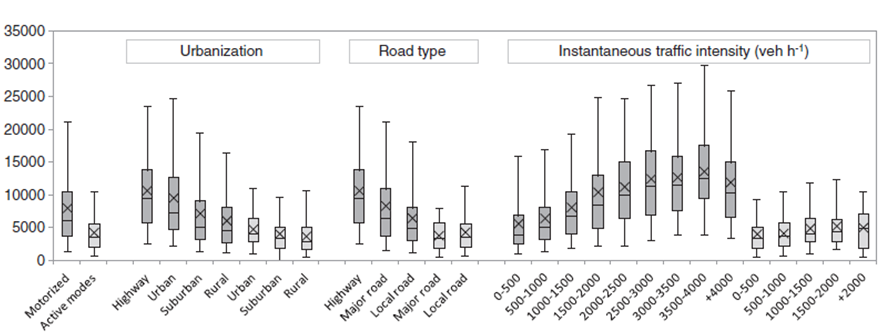
\includegraphics[scale=1]{road_type_exposure}
\caption{External factors affecting in-car black carbon exposure ($\mu \text{g m}^{-3}$). Vehicles are the dark boxplots. Walking are light}
\label{fig:road_type_exposure}
\end{figure}

By taking all the factors studied by Dons, a regression model of car I/O ratios for black carbon was developed and is shown in Figure \ref{fig:transport_io_ratios}.

\begin{figure}[H]
\centering
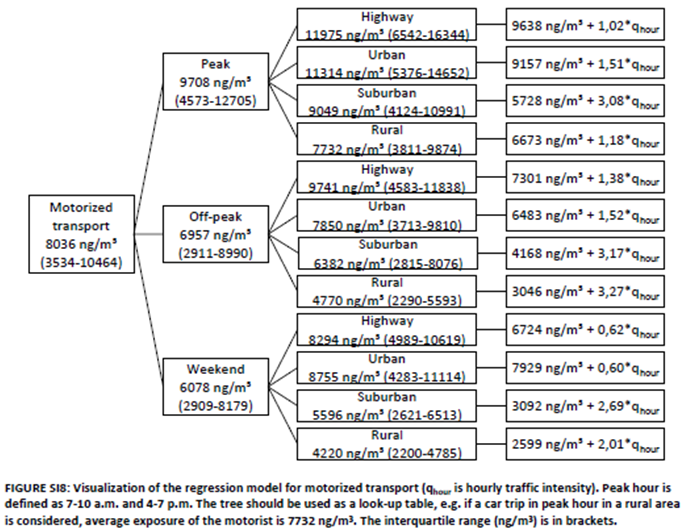
\includegraphics[scale=0.9]{transport_io_ratios}
\caption{Transport indoor/outdoor ratios}
\label{fig:transport_io_ratios}
\end{figure}

However the use of these ratios are not well tested and do not agree well with other ratios from the literature. It seems that given other known influences such as ventilation systems that a deterministic model based only on time of day and road type is too simplistic. For example in two studies by Gulliver and Briggs (\cite{Gulliver2004} and \cite{Gulliver2007}) particulate matter concentrations inside cars in Northampton and Leicester were roughly 30\% higher than concentrations at nearby monitoring stations. A table of mean concentrations from the 2004 paper are shown below in Table \ref{tab:gulliver_vehicle_means2}).

\begin{table}[H]
\caption{In-vehicle \gls{pm} concentrations}
\centering
    \begin{tabular}{ | l | l |}
    \hline 
     \bfseries{\gls{pm} Fraction} & \bfseries{Mean ($\mu \text{g m}^{-3}$)} \\ \hline
     \gls{pm10} & 43.16\\ \hline
     \gls{pm25} & 15.54\\ \hline
    \end{tabular}
\label{tab:gulliver_vehicle_means2}
\end{table}

The main conclusions from studies on in-car expose were that exposure is significantly influenced by traffic intensity and ambient air pollutant concentrations (being strongly linked to each other) as well as the choice of ventilation used inside the vehicles themselves. Is is a complicated picture. Estimating the exposure of individuals from the time they spend in the car micro-environment should take into account the factors outlined to try and as accurately as possible reflect reality.

%%%%%%%%%%%%%%%%%%%%%%%%%%%%%%%%%%%%%%%%
%%%%%%%%%%%%%%% CYCLING %%%%%%%%%%%%%%%%
%%%%%%%%%%%%%%%%%%%%%%%%%%%%%%%%%%%%%%%%

\subsubsection{Bicycle}
\label{sec:bicycle}

Between 2001 and 2011 the number of people living in London that cycled to work more than doubled from 77,000 to 155,000. Over the same time period there were also large increases in other large UK cities; Brighton by 109\%, Bristol by 94\%, Manchester by 83\%, Newcastle by 81\% and Sheffield by 80\% (\cite{OfficeforNationalStatistics2014}). This rise in cycling is normally attributed to a number of factors including local authorities building more cycle-friendly infrastructures, the promotion of cycling as a way to keep fit (supported by the Governments cycle-to-work discount scheme), and the public generally becoming more environmentally-aware. 

In some cities bicycle sharing systems have also contributed to this rise in cycling journeys. In London the Barclays Cycle Hire scheme was launched in July 2010 with around 5,000 (now around 11,000) bikes distributed around London at specially installed docking stations (\cite{TransportforLondon2014}). Similar systems operate in many places around the World. Although there is no definitive list as new schemes are opening all the time, in 2013 \cite{larsen2013bike} estimated there were more than 500 cities in 49 countries hosting advanced bike-sharing programs, with a combined fleet of over 500,000 bicycles (compared to 213 schemes in 2008 (\cite{Wikipedia2014})).

The \cite{Karanasiou2014} review looked at cycling exposure in 20 European studies, mostly in the \gls{uk} and the Netherlands. They found mean exposure values for \gls{pm25} of 29--72 $\mu \text{g m}^{-3}$ and for \gls{pm10} of 37-62 $\mu \text{g m}^{-3}$. The studies based in London (\cite{Kaur2005} and \cite{Adams2001}) found that cycling exposure to \gls{pm25} depended on the route taken, finding busier routes with more traffic increased cycling exposure. \cite{Ragettli2013} found similar - bicycle travel along main streets between home and work place contributed 21\% and 5\% to total daily ultra-fine particle exposure in winter and summer, respectively, and that exposure could be reduced by 50\% if main roads were avoided. At odds with this, the Netherlands study (\cite{Zuurbier2010}) found no difference between routes. Though in their methods it seems that there was overlap between the low-traffic and high-traffic routes, and also that their low-traffic routes were only low on car traffic and they were frequently used by mopeds, which may explain this difference.

The main variable common in studies of cycling exposure seems to be location. A cyclist riding in the middle of a busy road will be exposed to higher concentrations than on a separate cycle-lane, or a back-street. Given cyclists are not enclosed in any sort of vehicle this direct relationship between air pollutant concentrations and exposure is to be expected, as the cyclist is in closer proximity to the main sources (car exhausts).

With regard to the negative health impacts of exposure to poor air quality while cycling, unlike other transport modes such as car and bus, a number of recent studies have tried to quantify this. \cite{Woodcock2014} used Barclays Cycle Hire data from Transport for London (\gls{tfl}) to model the health impact for 578,607 people in London, mostly (78\%) aged between 14 and 45. They used the bike hire usage data, modelled the journeys between the docking stations, and combined this with general travel data, data on physical activity levels and road collisions, and finally 20 m by 20 m grids of annual average \gls{pm25} data. Cycling exposure was compared to replacing those journeys with walking or public transport. They found that the population benefits from the cycle hire scheme substantially outweighed the negatives, with a net change of minus 72 daily adjusted life years (\gls{daly}s) among men and minus 15 for women (negative \gls{daly}s represent a health benefit). In a very similar study in Barcelona \cite{Rojas-Rueda2013} did a Health Impact Assessment (\gls{hia}) for eight different scenarios where the the population of Barcelona was presumed to change transport mode from car to either cycling or public transport. Traffic incidents, physical activity and air pollution exposure were then estimated for each scenario and the relative health changes estimated in \gls{daly}s. For the scenarios where 20\% and 40\% of car trips where replaced by cycling trips, there were changes of minus 138 and minus 275 \gls{daly}s. Rather than doing a health impact assessment \cite{Nwokoro2012}, back in London, did more direct assessments of cycling exposure by looking at the amount of black material in the airways of non-cyclists and cyclists. They found that commuting to work by bicycle in London was associated with increased long-term inhaled dosage of black carbon, however the relationship was difficult to properly quantify. This was because cycling typically takes longer for those people to cycle to work than, for example, a train journey. Route choice further complicates matters as although being away from highly polluted routes lowers exposure, the increased journey time may increase total exposure over the trip. Figure \ref{fig:airway_cycling_blackcarbon} (from \cite{Nwokoro2012}) below shows the increased macrophage carbon measured in cyclists compared to non-cyclists (A macrophage is a cell responsible for destroying harmful pathogens).

\begin{figure}[H]
\centering
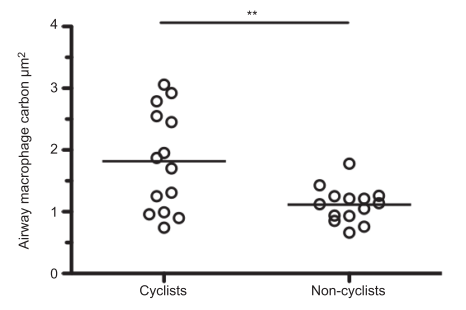
\includegraphics[scale=0.6]{airway_cycling_blackcarbon}
\caption{Airway macrophage carbon in cyclists and non-cyclists}
\label{fig:airway_cycling_blackcarbon}
\end{figure}

In summary cycling exposure is very dependant on the routes taken by cyclists, and their position on the road. The negative health effects of cycling have been explored in comparative transport mode studies showing that when taken alongside other variables such as risk of injury, cycling has health benefits. There are a lack of studies that take cycling exposure as part of a larger daily exposure health assessment alongside other transport modes and indoor micro-environments. A number of the health studies are encouraging in that they do model sufficiently large groups of people to draw epidemiological conclusions but only the transport aspect of these people's exposure is explored rather than cycling in the context of their daily typical exposure. Also there are other parts of their models which could be improved, for example the studies in London and Barcelona only used annual average air quality concentrations (rather than daily or hourly for example).

%%%%%%%%%%%%%%%%%%%%%%%%%%%%%%%%%%%%%%%%
%%%%%%%%%%%%%%%% TRAINS %%%%%%%%%%%%%%%%
%%%%%%%%%%%%%%%%%%%%%%%%%%%%%%%%%%%%%%%%

\subsubsection{Train travel}
\label{sec:train}

In their 2014 review of commuter exposure in Europe (which has been referred to extensively in this section on transport exposure), Karanasiou did not review train travel -- focusing on cycling, cars and underground subway systems. However \cite{Nasir2009}, \cite{Colbeck2010a}, \cite{Dons2011}, \cite{Ragettli2013} and \cite{Knibbs2011} all have elements of their publications which take train travel exposure as a separate travel micro-environment.

\cite{Nasir2009} and \cite{Colbeck2010a} found concentrations during peak journey times in air-conditioned carriages were 44 $\mu \text{g m}^{-3}$, 14 $\mu \text{g m}^{-3}$ and 12 $\mu \text{g m}^{-3}$ for \gls{pm10}, \gls{pm25} and PM$_{1}$ respectively, but that during off-peak times, concentrations were about half this. Concentrations were lower again in non-air conditioned carriages. They drew the conclusions that particulate levels inside trains are strongly influenced by the numbers of passengers and that their movement and presence causes particle re-suspension. Peak travel times (when there are more passengers) coincided with higher particulate concentrations. Figure \ref{fig:nasirtrainstops} (from \cite{Nasir2009}) shows the effect of train stops on concentrations in the train cabin. It would have been interesting to see simultaneous outdoor concentrations to see how they varied to the indoor concentrations and more detailed information on passenger numbers. It might be that outdoor concentrations contribute to a certain percentage of the indoor concentrations, which are then varied positively or negatively by passenger numbers.

\begin{figure}[H]
\centering
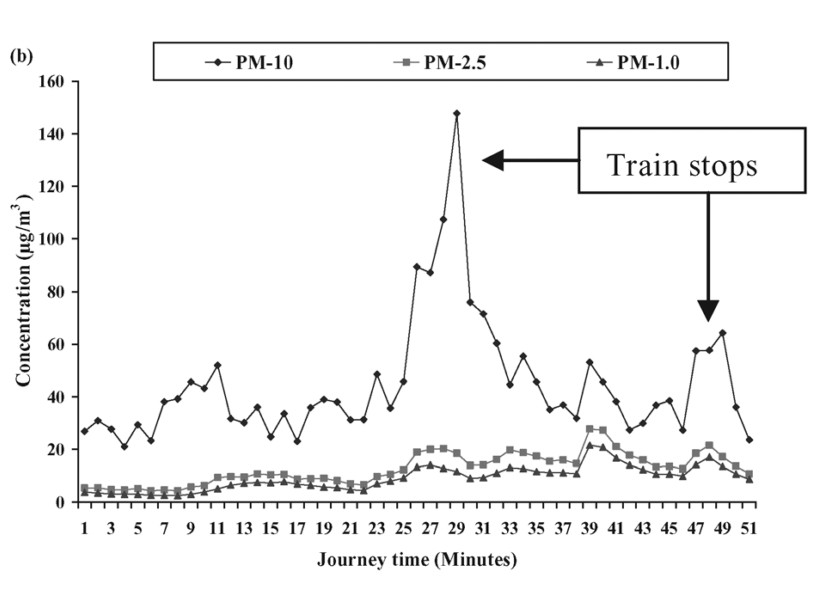
\includegraphics[scale=0.4]{nasir_train_stops.png}
\caption{Train stops and train exposure}
\label{fig:nasirtrainstops}
\end{figure}

\cite{Knibbs2011} reviewed articles to look at the difference between diesel and electric powered trains, and based on the limited data available found that the power source of the rail vehicle appears to strongly affect ultra-fine particle concentrations (diesel powered trains have higher in-train particle concentrations than electric trains). High concentrations of particles are not just confined to the trains themselves either, \cite{Ragettli2013} found \gls{ufps} levels within train stations twice as high as suburban background and nearby residential streets in Basel, Switzerland.

In summary the variables that drive exposure levels on trains are the fuel source, the number of stops that the train makes, the influx of passengers at those stops, and the concentrations outside of trains. No research on specifically how train travel exposure affects the health of passengers was found. As with the other transport modes reviewed thus far, a model which incorporates these variables alongside other micro-environments should be able to develop a more accurate picture of human exposure over days or weeks.


%%%%%%%%%%%%%%%%%%%%%%%%%%%%%%%%%%%%%%%%
%%%%%%%%%%%%% UNDERGROUND %%%%%%%%%%%%%%
%%%%%%%%%%%%%%%%%%%%%%%%%%%%%%%%%%%%%%%%

\subsubsection{Underground subway systems}
\label{sec:underground}

% General underground stuff.

In many worldwide cities the population travel between locations using metro systems. The London Underground was the first such system to open in 1863, but other cities have followed including New York, Paris, Seoul, Beijing, Berlin and Madrid. The size of each system varies in size, as does the power source, depth and speed of the trains, however the systems tend to be almost unanimously popular as a choice of travel mode for commuters.

The \cite{Karanasiou2014} review found 12 studies that had measured exposure in subway systems. Particulate levels were found to be generally highest on the platforms of the system, compared to inside the vehicles themselves. Exposure was also generally higher during peak travel times. Mean \gls{pm10} levels were in the range of 103 to 1030 $\mu \text{g m}^{-3}$, and \gls{pm25} levels between 59 and 375 $\mu \text{g m}^{-3}$. The highest levels were found in London, Stockholm and Rome. Variation between and within systems was thought to be explained by different brakes types, air-con or natural ventilation systems, different types of rails, and the numbers of trains. A summary table from the review is shown in Figure \ref{fig:pm_tube_summary} (from  \cite{Karanasiou2014}).

\begin{landscape}
\begin{figure}[H]
\centering
\frame{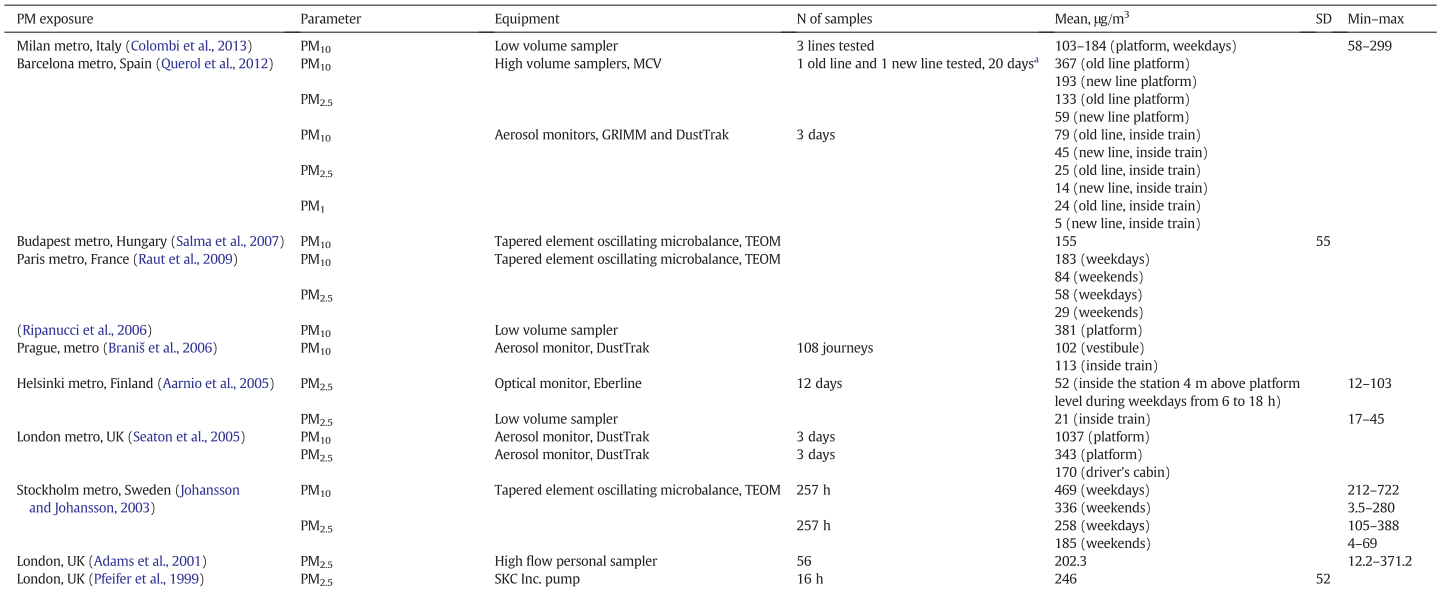
\includegraphics[scale=0.6]{pm_tube_summary}}
\caption{Summary of underground subway studies}
\label{fig:pm_tube_summary}
\end{figure}
\end{landscape}

Focusing specifically on London, the work of Adams in the late 1990's \slash early 2000's is oft cited and well known in this area of transport exposure due to it being the first comprehensive particulate matter multi--mode transport user exposure assessment study in the \gls{uk}. They measured a large number of journeys (465) across many modes (bicycle, car, bus, tube) over different periods in July 1999 ('summer') and February 2000 ('winter') finding mean \gls{pm25} values for the London Underground of 247.2 $\mu \text{g m}^{-3}$ in summer and 157.3 $\mu \text{g m}^{-3}$ for the winter (or an overall mean of 202 $\mu \text{g m}^{-3}$ as shown in the Figure \ref{fig:pm_tube_summary}). Shortly after this publication another paper was published by the same group which tried to apportion the PM to sources (\cite{Adams2001a}). They concluded that most of the \gls{pm} came from metals from sources such as braking, tyre wear and the tracks. A high iron content was found. They noted that the \gls{pm} in the underground should not be directly compared with \gls{pm} above ground as it's composition is very different. In terms of the actual levels measured in the first paper however extrapolation of these measures across the entire underground network including within cabins and on the platforms is not proven. \cite{Seaton2005} found large variations between \gls{pm} in cabins and on the platforms themselves. In their research (funded by the London Underground to look at at occupational health exposure to \gls{pm25}) platform concentrations were 270–-480$\mu \text{g m}^{-3}$ and cab concentrations were 130–-200 $\mu \text{g m}^{-3}$. Similarly high to the other studies of the London Underground. This paper also found a high iron content in the \gls{pm} of 67\%. Seaton summarises however that although the concentrations are high, they are unlikely to represent a health risk to workers due to daily time-weighted exposure calculations. \cite{Loxham2013} disagrees. Their research was not included in the Karanasiou review (presumably due to it being published only shortly before the review). They looked at \gls{pm10}, \gls{pm25} and PM$_{0.1}$ composition finding similar to the other research, that the particles are mostly from interaction between wheels, rails, and brakes with a high iron content. However they suggest that the potential health effects of exposure to the ultrafine fraction of underground \gls{pm} warrants further investigation, as a consequence of its greater surface area/volume ratio and high metal content.

% LU summary bit.

To summarise, exposure and the related health effects of poor air quality in subway systems has not been extensively studied in most cities. Certainly not to the point where researchers can confidently say what levels of particulate matter the public are being exposed to at different times of the day, in different places of the underground, and what composition that has (and how toxic to the body it is or is not). What can be fairly confidently said however is that concentrations in most systems, and certainly in London, are higher than street-level, in-vehicle, cycling, buses or most other studied transport micro-environments. Although the composition is very different and may be more or less toxic. Due to the number of people that use this transport mode daily (1.171 billion journeys annually in London according to \cite{TransportforLondon2014a}) for extended periods of time, understanding and being able to quantify exposure during it is necessary to better estimate people's daily exposure across a range of micro-environments. Certainly they vary hugely from concentrations measured at a subjects place of residence, as is used in the static exposure studies considered earlier.

\subsubsection{Transport exposure summary}
\label{sec:trans_exposure_summary}

Studies of exposure while people are in-transit between locations using transport modes such as cars, trains, subway systems and bicycles shows a large range of concentration values. There are few exposure studies which account for these variations (alongside outdoor indoor infiltration) to provide exposure data on the daily lives of large numbers of subjects suitable for epidemiological analysis. Until more expansive exposure studies that follow large groups of people of varying time-activity patterns are completed, the ability to discern the range of commute-time’s specific contribution to total exposure is constrained (\cite{Knibbs2011}).

%%%%%%%%%%%%%%%%%%%%%%%%%%%%%%%%%%%%%%%%
%%%%%%%%%%%%%% MODELLING %%%%%%%%%%%%%%%
%%%%%%%%%%%%%%%%%%%%%%%%%%%%%%%%%%%%%%%%
\newpage

\subsection{Dynamic and Hybrid exposure models}
\label{sec:dynamic_hybrid_models}

Section \ref{sec:staticexposurehealth} (Static exposure studies) concluded that taking fixed-point or fixed-area measurements, often at one point in space or time, was insufficient to accurately quantify human exposure to air pollution. Exposure varies in space and time due to an individual’s activities, the time of day, and the location of the subject. Poor air quality an individual is exposed to will vary depending on how long they spend in public transport each day (and which mode of transport), how long they spend at home or at work, and the concentrations within those environments themselves (\cite{Ozkaynak2013}). Therefore one approach would be to deploy personal monitors to large numbers of people, then aggregate and analyse the data to better understand how exposure varies between people and environments.

Section \ref{sec:personal_monitoring} (Personal monitoring) considered how personal monitoring devices can be used to do this; to better understand individual-level exposure to poor air quality and the drivers thereof. However it concluded by discussing how collecting large enough quantities of accurate data using this method is extremely difficult to do. The following Sections of \ref{sec:infiltration} (Infiltration) and \ref{sec:transport} (Transport) looked at modelling approaches which enable researchers to quantify exposure to populations in those specific environments (and some discussed the health implications of those environments), but they were not 'joined-up' so as to enable estimates of individuals total daily/annual exposure alongside other micro-environments and times of the day/year.

This section now looks at a small number of research studies which are also modelling approaches, but that try to be more holistic in their exposure assessments, including many micro-environments as well as temporal and spatial variation of the subjects and air quality as inputs. 

Models are of course an abstraction of the real world, and as such will almost certainly never represent it with 100\% accuracy, but using these methods it is possible to simulate the movements and exposure of a much larger number of subjects than would be possible otherwise. By being aware of the inaccuracies and drawbacks of the model and model inputs, it is also possible to quantify the error and propagation of error, and take this into account for any subsequent health impact studies. For example one key input to an air quality exposure model will normally be an air quality model. This can be evaluated against monitoring site data, and the RMSE noted, then calculated alongside other model parameters to understand the overall model uncertainty. This said, an area of the model which would be difficult to quantify in this manner is the spatial aspect. When modelling the movements of a individual it is hard to numerically quantify this in a form that can be included with the other model uncertainties. If an individual takes one route to work, but the model predicts another, this would be a difficult error to propagate due to the different units being used (metres rather than pollutant concentrations).

This is a new area of research which is not yet established, and the nomenclature is thus still under development, but a trend towards discussion of 'hybrid' or 'dynamic' models has emerged. 'Hybrid' being a description of a combining of multiple approaches of exposure, such as time-activity diaries combined with modelled air quality data and micro-environmental modelling of transport modes, and 'Dynamic' reflecting the improved temporal scale of data available, for both the populations movement and the variation in pollutant concentrations. 

The following sections are samples of current publications in this field to provide a 'baseline' for the model that this research describes. \cite{Kousa2002}, \cite{Dhondt2012}, \cite{DeNazelle2013}, \cite{Gerharz2013} and \cite{Reis2018} all attempt, with varying degrees of complexity, to model exposure of individuals over an entire day (rather than using measurements or only considering one micro-environment).

%%%%%%%%%%%%

\subsubsection{Kousa et al}
\label{sec:dynamic_models_kousa}

\cite{Kousa2002} was a very early attempt at this sort of model. They evaluated the temporal and spatial exposure of the population of the Helsinki Metropolitan Area in different micro-environments (home, workplace, traffic and other). For time-activity data (15 min resolution) they used 435 diaries from the EXPOLIS study, and they then linked this to modelled \gls{no2} data from a dispersion model which outputted grids of 500 m by 500 m for the greater Helsinki area, and 50 m by 50 m for the city centre. For indoor environments they took an I/O ratio of 0.76, including when the subjects were recorded as being in transport. The \gls{gis} technology and spatial analysis techniques used in this model would have been quite advanced at the time, and therefore modelling the exposure of 8000 people was impressive. Specifically, modelling the air quality with hourly variation and at 50 m resolution. However in-light of contemporary work this model is simplistic in a number of ways including: only describing four micro-environments (and using the same I\slash O ratio for all of them), that the time-activity diaries are only at 15 minute intervals, that the data only includes people of ages 25-55, and that they only modelled weekdays. It would also have been interesting to see what difference using this model made on exposure assessment i.e. a comparison with monitoring sites or address-points, such as the research by \cite{Dhondt2012}.

\subsubsection{Dhondt et al}
\label{sec:dynamic_models_dhondt}

Based in Belgium \cite{Dhondt2012} compared 'static' and 'dynamic' models for exposure to \gls{no2} and \gls{o3}, modelling their subject's behaviours and location based on 8800 activity diaries and 12 km location 'zones', then scaling this to give results relevant for 5 million people. For their air quality inputs hourly concentrations were modelled using a variety of nested models, giving higher resolution nearer to roads and in urban areas, and lower resolution outside of these areas. Time in transport in each zone was also included. Maps showing the exposure over 24 hours accumulated by each zone are shown in Figures \ref{fig:dhondt_static_exposure} and \ref{fig:dhondt_dynamic_exposure}.

\begin{figure}[H]
\centering
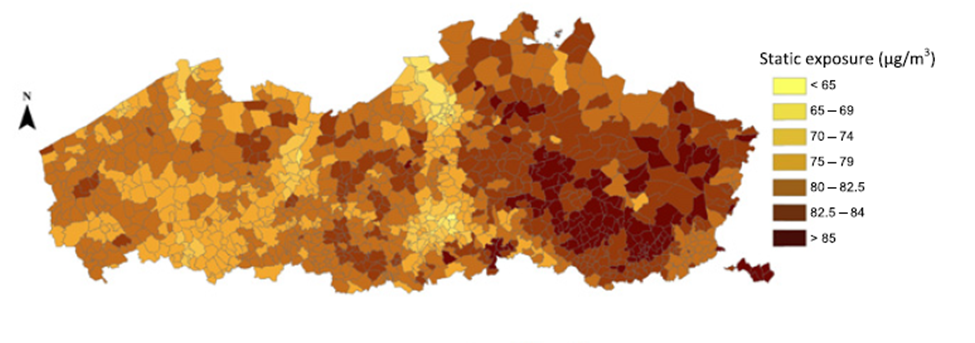
\includegraphics[scale=0.9]{dhondt_static_exposure}
\caption{\gls{no2} static exposure results}
\label{fig:dhondt_static_exposure}
\end{figure}

\begin{figure}[H]
\centering
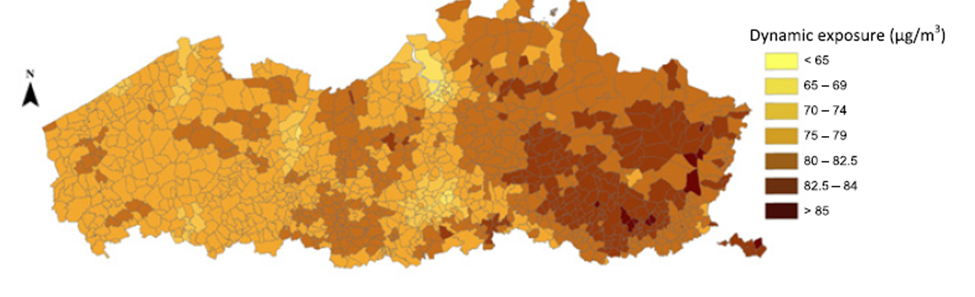
\includegraphics[scale=0.9]{dhondt_dynamic_exposure}
\caption{\gls{no2} dynamic exposure results}
\label{fig:dhondt_dynamic_exposure}
\end{figure}

By using this approach to exposure modelling they found \gls{no2} was being underestimated by on average 1.2\%, and that \gls{o3} was being overestimated by 0.8\%. These do not seem particularly large differences, however as an input to a large cohort of subjects in a long time-series analysis they could significantly change any health conclusions. These regional averages also mask much of the variation in individuals, where differences of upto 12\% can be found depending on age group, gender and place of residence. Having studied the methods however, the reliability of the results is open to question. This research is certainly moving towards the type of dynamic exposure model described earlier, as their modelled air quality and time-activity data is of a high quality, however there is no micro-environmental modelling at all, which given the time that we know people spend indoors, must be a large source of uncertainty in the results. As a final note on this publication, the method of grouping the exposure results into time-activity zones rather than by residence of the subject was interesting and informative, showing the areas where greatest miss-classification occurred in a visual and effective manner.

%%%%%%%%%%%%
%% Study uses modelling of air quality and adjustments for micro-environments.
%% But difficult to upscale and relies on alot of context thus not good.

\subsubsection{de Nazelle et al}
\label{sec:dynamic_models_denazelle}

The following year \cite{DeNazelle2013} did a similar study for 7 days of 36 subjects in Barcelona, however in addition to using time-activity diaries as an input, the subjects also had software installed on a provided smartphone, which made use of the accelerometer and \gls{gps} hardware to record their location and infer their type of activity. After substantial processing of this data, the subjects location and activity was linked with an hourly resolved 5 km x 5 km dispersion model grid of \gls{no2}, and personal exposure was then calculated, including adjustments for six different micro-environments (indoor, bike, bus and tram, car and taxi, metro and train, motorcycle). This study was truly a hybrid study, in that data was collected using personal monitoring (smartphones) but then joined with modelled data and further processing of the data. De Nazelle then calculated the time that the subjects spent in different micro-environments, and compared this to the percentage of their daily exposure in the same micro-environment categories (Figure \ref{fig:time_no2_activity_spaces}).

\begin{figure}[H]
\centering
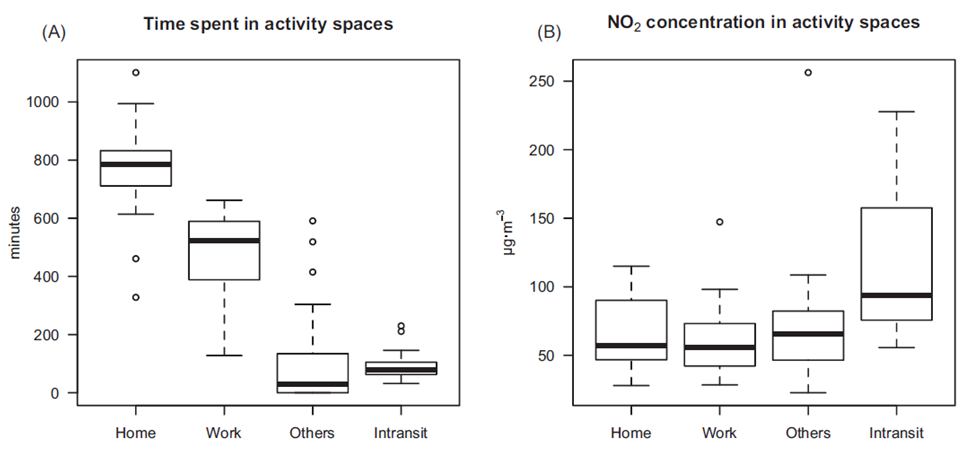
\includegraphics[scale=0.8]{time_no2_activity_spaces}
\caption{Time and \gls{no2} in activity spaces}
\label{fig:time_no2_activity_spaces}
\end{figure}

From the results we can see that the subjects spent most of their time at home and at work (left), supporting the use of static exposure models where these fixed locations are used, however when the actual exposure is considered the influence of the time spent in those locations diminishes (right) and 'Others' and 'In-transit' become important (supporting the conclusions of \cite{Dons2011} discussed in Section \ref{sec:transport}, '\nameref{sec:transport}'). The study concludes by discussing how these techniques could be developed and used for much larger populations (presumably as an input to health studies eventually). However the amount of post-processing of the geographical data, the manual translation of activity diaries to compliment the smartphone data, and the extra battery packs that needed adding to the phones makes this seem less likely. To upscale this to many hundreds or thousands of subjects would need a tremendous amount of coordination and equipment which would need to be distributed, collected and monitored. The data processing would also seem to be difficult without large human resources, and linking to health outcomes would mean the study needed to be designed so that the participants are a statistical representation of the wider study area population, or the numbers surveyed so close to the actual study population that they give a good representation anyway. 

%%%%%%%%%%%%
\subsubsection{Gerharz et al}
\label{sec:dynamic_models_gerharz}

In the same year \cite{Gerharz2013} used similar methods to examine the exposure of 10 people in Munster, Germany. They used activity diaries alongside \gls{gps} data again, defined micro-environments using this contextual information of 'home', 'work', 'other indoor', 'transportation', and 'outdoor', joined this to an hourly average \gls{pm10} dispersion model for the air quality input, and then used I/O ratios for the micro-environments e.g. 1.34 for cars and 2.49 for public transport. The model is summarised in Figure \ref{fig:gerharz_exposure_diagram} below.

\begin{figure}[H]
\centering
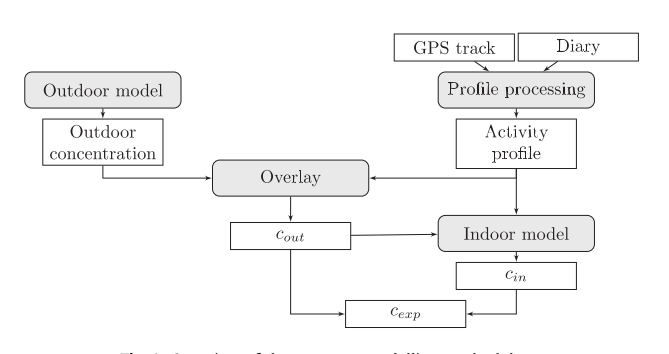
\includegraphics[scale=0.8]{gerharz_exposure_diagram}
\caption{The exposure process}
\label{fig:gerharz_exposure_diagram}
\end{figure}

The major difference between this and the work of De Nazelle and Dons is that they also gave the subjects personal air quality monitoring data in the form of a Grimm Aerosol Spectrometer. The spectrometer provided information about particle numbers and mass in 32-size classes with a high temporal resolution of 6 seconds. Using this data they were able to evaluate the effectiveness of their modelled exposure by comparing it to real data. The Pearson’s correlation coefficient between the mean of modelled and measured data is shown in Figure \ref{fig:gerharz_results}.

\begin{figure}[H]
\centering
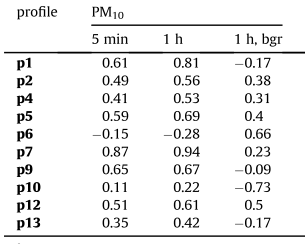
\includegraphics[scale=1]{gerharz_results}
\caption{Pearson’s correlation coefficient between the mean of modelled and measured data}
\label{fig:gerharz_results}
\end{figure}

There is clearly some variation between the results, with P7 (person 7) being particularly strong, and P10 being particularly weak. Gerharz notes that "Generally, the correlation between model average and measurements is high" which does not seem to tally with the mean of their correlations coming out as 0.44. However they are correct in saying that it does at least "clearly outperform the baseline approach of using urban background measurements as proxy for the personal exposure". Though in terms of using this modelled approach for larger groups of people, the post-processing of \gls{gps} data and activity-diaries, general data cleaning, and data linkage would seem to make this an unlikely approach (as with \cite{DeNazelle2013})

%%%%%%%%%%%%
\subsubsection{Reis et al}
\label{sec:dynamic_models_reis}

The most contemporary study to the development of this research is the exposure modelling undertaken by \cite{Reis2018}. They combined hourly 1km by 1km estimates of air quality (for the whole of the UK) with 1km by 1km estimates of 'workday' population density v. 'home' population density (based on the UK Census 2011 and the UK Land Cover Map 2015). Calculating exposure for when the population is at home, compared to when they are at home + when they are at work. Given this study modelled the entire UK populations exposure, in a 'dynamic' way, this is a very impressive piece of research; at a much larger scale than any of the previous studies mentioned in this section and with high temporal air quality resolution. This approach has the benefits of being readily transferable to other countries in the world (where similar census and data exist, which are not uncommon), however it could be improved by a) including commute time/mode of transport in the exposure estimates b) including exposure/time spent in indoor microenvironments and c) by modelling movement and air quality at a finer scale than 1km. The model also only allows exposure statistics to be calculated at an aggregate level, making individual exposure estimates difficult, though perhaps example distributions for each 1km grid could somehow be included with further data manipulation.

%%%%%%%%%%%%
\subsubsection{Dynamic and hybrid model reviews}
\label{sec:dynamic_models_reviews}

\cite{Ozkaynak2013}, \cite{Meliker2011} and \cite{Baxter2013} have written reviews / position statements on this type of research. Ozkaynak's diagram below (Figure \ref{fig:ozkaynak_exposure_diagram}) is useful for summarising how the complexity of exposure modelling has advanced, and with the complexity the inputs required.

\begin{figure}[H]
\centering
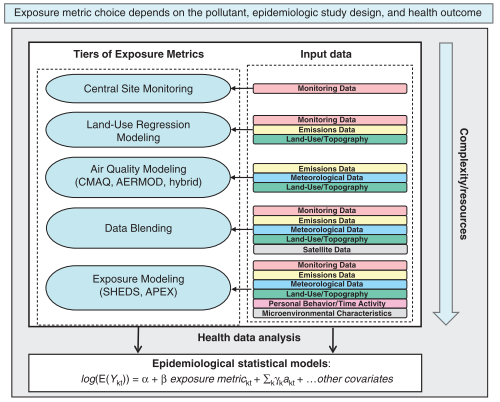
\includegraphics[scale=1]{ozkaynak_exposure_diagram}
\caption{The evolution of exposure assessment}
\label{fig:ozkaynak_exposure_diagram}
\end{figure}

They concluded that these new approaches can help refine the significance of air pollution health outcomes, but that this will depend on study-specific characteristics, including epidemiological study design (e.g., time-series vs cohort), the form of of health outcome being considered (e.g., long-term or short-term), which pollutants, and the role of pollutant and building specific indoor infiltration and human activity patterns. \cite{Meliker2011} offers a slightly different but useful perspective, by identifying what they consider are the five most important domains to the development of improved spatio-temporal epidemiological models, namely:

\begin{enumerate}
  \item spatio-temporal epidemiologic theory
  \item selection of appropriate spatial scale of analysis
  \item choice of spatial/spatio-temporal method for pattern identification
  \item individual-level exposure assessment in epidemiologic studies
  \item assessment and consideration of locational and attribute uncertainty
\end{enumerate}

\cite{Baxter2013} summarises this emerging area of research well by explaining how, when compared with the use of central-site monitoring data (or other fixed-location methods) the enhanced spatial (and temporal) resolution of air quality or exposure models can impact on resultant health effect estimates, especially for pollutants derived from local sources such as traffic.  They recommend that future research develops pollutant-specific infiltration data, improves existing data on human time-activity patterns and exposure to local sources, in order to enhance human exposure modelling estimates. Also that these new approaches are compared with existing approaches to exposure estimation to better characterise estimates in chronic health studies. This research attempt to take this field forward as described.

%%%%%%%%%%%%
Figure \ref{fig:james_exposure_diagram} is proposed as a conceptual model of a hybrid/dynamic exposure model, in response to the review of the field by \cite{Baxter2013} and having reviewed the literature in the field during Section \ref{sec:dynamic_hybrid_models}. The model should have highly temporal and spatially resolved air quality inputs which consider both indoor and outdoor sources (including regional and local source for the latter), it should be able to model infiltration rates for different modes of transport and building types, it should reflect the multiple micro-environments that people spend their time in (and take account of the temporal resolution of these) and finally it should (for linkage through to epidemiological end-points) be able to consider different breathing rates to quantify exposure and dose for multiple pollutants.

\begin{figure}[H]
\centering
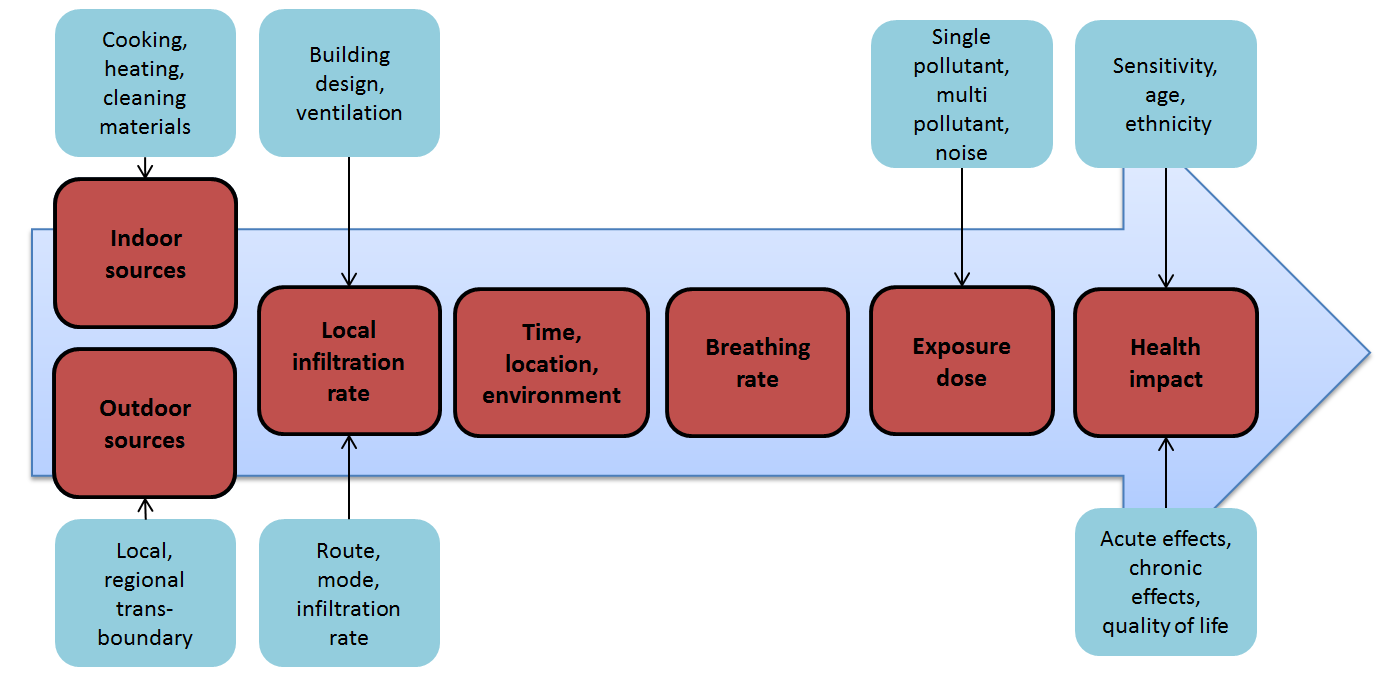
\includegraphics[scale=0.4]{james_exposure_diagram}
\caption{A conceptual dynamic exposure model}
\label{fig:james_exposure_diagram}
\end{figure}

\section{Research aims and objectives}
\label{sec:intro_aims_and_objectives}

Having reviewed literature in the field of dynamic or hybrid air quality exposure modelling, and the general background areas of air quality and health, with the above model in mind, the hypothesis this research proposes is that "\textit{Individual and population level air pollutant exposure can be estimated using time-activity surveys, \gls{gis} and routing tools, coupled with high resolution spatio-temporal air quality models, facilitating a greater understanding of the exposure to air pollution in an urban environment}". The research was structured around four primary aims as follows:

\begin{enumerate}
\item Reconstruct the time-space activity of London's population
\item Link modelled air quality, estimate exposure, and compare with traditional methods
\item Refine the models estimates of London Underground exposure
\item Evaluate the results
\end{enumerate}

Exposure on the London Underground was focused on in the third results chapter (as oppose to exposure in other environments) due to it becoming apparent during chapter two that the concentrations in this environment are some of the highest that Londoners are exposed to during their typical days.

In more detail the movements of the subject's in the \gls{tfl} dataset will be modelled, their days reconstructed on a fine temporal and spatial scale, and this data used in conjunction with a novel exposure model. The air quality input used was the \gls{cmaq}-UK model (see Section \ref{subsec:cmaq_urban}). The results of the model allowed interrogation of exposure by individual, or grouped by various demographics, which enable epidemiologists to increase their understanding of exposure miss-classification. Results are compared to static modelling approaches of the type discussed in Section \ref{sec:staticexposurehealth}. The model is then refined with personal monitoring on the London Underground, before an introduction to validation/testing of the results is presented. The objectives follow the work-plan below.

\subsection{Modelling Londoners movements}
\label{sec:modelling_londoners_movements}

\textbf{Aim} Create a model of Londoners daily movements based upon freely available TfL datasets

\textbf{Objectives}

\begin{enumerate}
\item Source, explore and identify key TfL flow datasets
\item Clean and import data to working environment
\item Complete any required modal specific routing (interrogation, querying, storage)
\item Quality assurance / quality check (QA/QC)
\item Analysis by demographic / geographical area
\end{enumerate}

\subsection{Dynamic exposure modelling}
\label{sec:dynamic_exposure_modelling}

\textbf{Aim} Model exposure to \gls{pm25} and \gls{no2} of the \gls{ltdsx} subjects, and compare with traditional exposure methods.

\textbf{Objectives}

\begin{enumerate}
\item Link population movement data to air quality data
\item Incorporate I/O ratios and micro-environmental factors
\item Create a postcode comparison dataset
\item Create a address-point comparison dataset
\item Create a monitoring site comparison dataset
\item Analysis
\end{enumerate}

Thus far, these aims cover the first half of the conceptual exposure model shown in Figure \ref{fig:james_exposure_diagram} (which is repeated here for convenience). 

\begin{figure}[H]
\centering
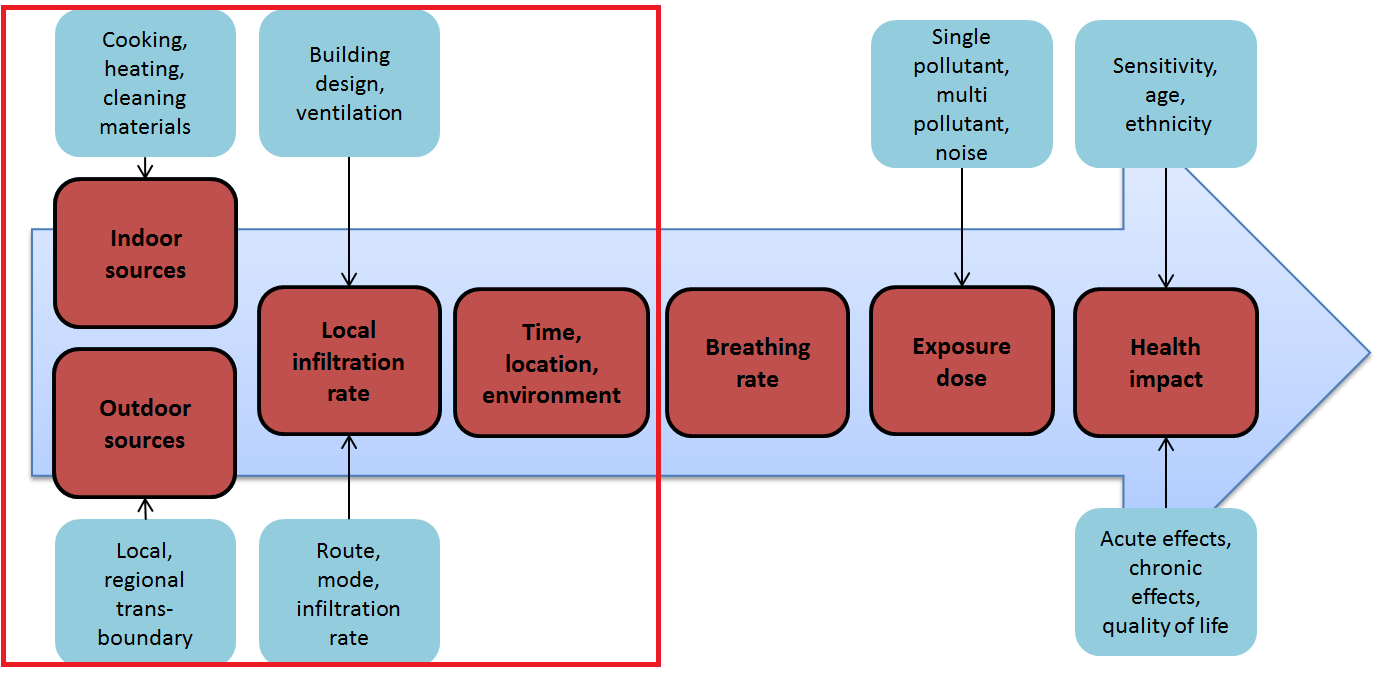
\includegraphics[scale=0.4]{james_exposure_diagram_v2}
\caption{A conceptual dynamic exposure model}
\label{fig:james_exposure_diagram_v2}
\end{figure}

The following two sets of aims and objectives focus on improving exposure estimates, and evaluating them respectively.

\subsection{Exposure to \texorpdfstring{PM$_{2.5}$}{} on the London Underground}
\label{sec:exposure_on_the_tube}

\textbf{Aim} Create an exposure model for exposure to \gls{pm25} on the London Underground

\textbf{Objectives}

\begin{enumerate}
\item Measure \gls{pm25} across the London Underground network
\item Link measured air quality data to noted time-location data
\item Import, process and clean other datasets for linking i.e. platform depths, station locations. 
\item Analysis
\end{enumerate}

\subsection{Evaluating dynamic exposure models}
\label{sec:evaluating}

\textbf{Aim} Develop an understanding of methods to evaluate predictions of exposure from hybrid-type models

\textbf{Objectives}

\begin{enumerate}
    \item Develop a data collection plan based on simulated and measured datasets
    \item Undertake mobile monitoring to collect data representative journey(s)
    \item Model exposure of the same journey(s)
    \item Analysis: compare the monitored and modelled exposures
\end{enumerate}
\label{chap:dynamic_exposure}

\chapter{My research aims}
The hypothesis of this research is that "\textit{Individual and population level air pollutant exposure can be estimated using time-activity surveys, GIS and routing tools, coupled with high resolution spatio-temporal air quality models, facilitating a greater understanding of the health impacts of air pollution and how public health risks can be reduced}". The research objectives that will need to be met to achieve this goal are as follows:

\begin{enumerate}
\item Reconstruct the time-space activity of London's population
\item Link modelled air quality, estimate exposure, and compare with traditional methods
\item Refine the models estimates of London Underground exposure
\item Evaluate the results
\end{enumerate}

In more detail I will model the movements of the subject's in the TfL dataset, reconstruct their days on a fine temporal and spatial scale, and then use this data in conjunction with a novel exposure model. The air quality input will be a CMAQ-UK model (see Section \ref{sec:cmaq_urban}. The results of the model will allow interrogation of exposure by individual, or grouped by various demographics, which will enable epidemiologists to increase their understanding of exposure miss-classification. Results will be compared to static modelling approaches of the type discussed in Section \ref{sec:staticexposurehealth}. The model will then be improved with personal monitoring on the London Undergound, before an introduction to validation/testing of the results will be undertaken. The objectives will be met by following the work-plan below:

\section{Reconstructing the  time-space activity of the population of London on a minute-by-minute basis from the London Transport Demand Survey (LTDS)}

\begin{enumerate}
\item Explore the LTDS dataset and identify key data
\item Move data from local Microsoft Access database into a PostgreSQL + PostGIS database
\item Clean data
\item Complete modal specific routing (interrogation, querying, storage) between origin and destinations
\item Quality check the routing results and do further data cleaning
\item Create and populate final dynamic location database table
\item Analysis of results
\end{enumerate}

\section{Link  air  quality  to  Londoner's  reconstructed  days (LTDS-X),  and  compare  with traditional exposure models }

\begin{enumerate}
\item Link data to CMAQ-Urban UK, incorporate IO ratios and micro-environmental factors (The 'LHEM')
\item Create a postcode comparison dataset
\item Create a address-point comparison dataset
\item Create a monitoring sites comparison dataset
\item Analysis and comparison of results
\end{enumerate}

Thus far, these aims cover the first half of the conceptual exposure model shown in Figure \ref{fig:james_exposure_diagram} (which is repeated here for convenience). The following two sections will be on improving exposure estimates, and evaluating them respectively.

\begin{figure}[H]
\centering
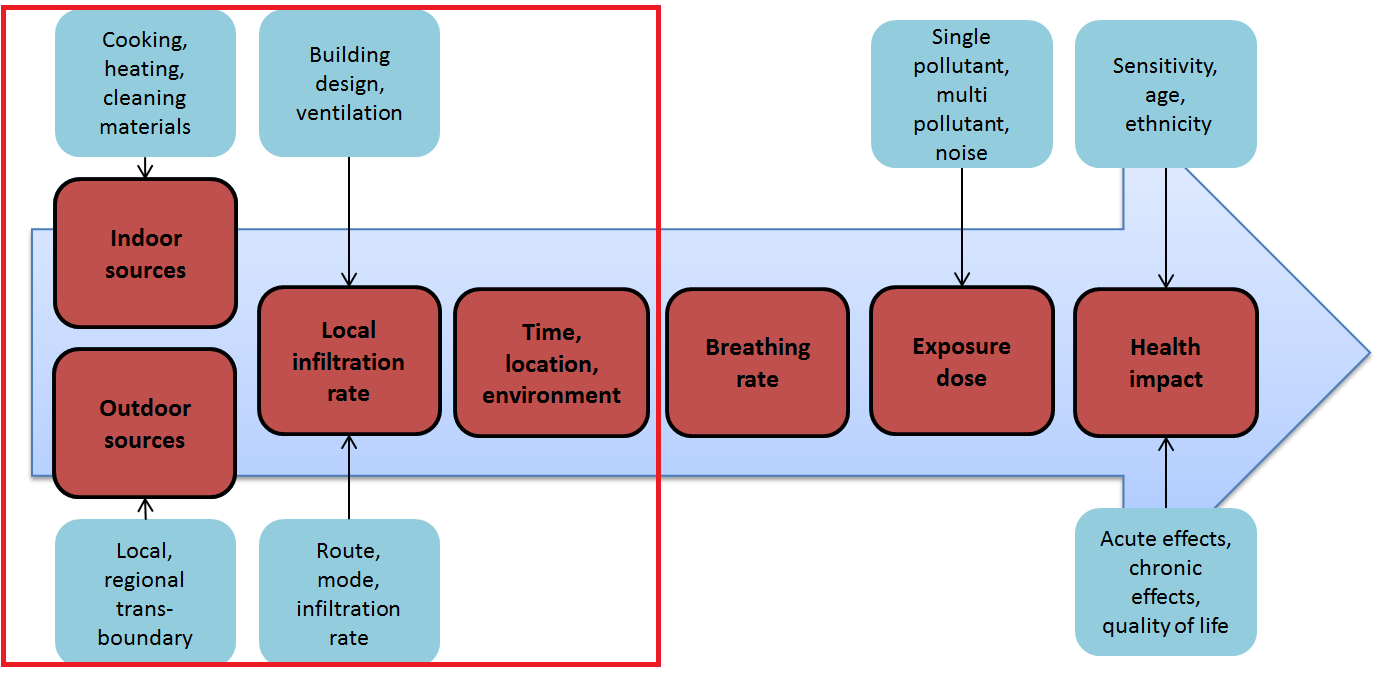
\includegraphics[scale=0.4]{james_exposure_diagram_v2}
\caption{A conceptual dynamic exposure model}
\label{fig:james_exposure_diagram_v2}
\end{figure}

\section{Exposure to \texorpdfstring{PM$_{2.5}$}{} on the London Underground}

\begin{enumerate}
\item Measure PM$_{2.5}$ across the London Underground network
\item Transcribe a time-location diary and link to pollutant data
\item Import other relevant data
\item Analyse data to characterise PM$_{2.5}$ on the London Underground
\end{enumerate}

\section{Evaluation of the dynamic exposure model using personal monitoring}

\begin{enumerate}
\item Use monitoring site data to estimate how many repeat journeys are required to estimate exposure on a specific route i.e. eliminate day to day variation
\item Select routes from the LHEM
\item Conduct repeated personal exposure monitoring on those routes
\item Compare outputs from LHEM to the personal exposure monitoring
\end{enumerate} 

\chapter{Methods and tools}
In order to complete the work required to meet my aims, various pieces of software, tools and methods are required. Appropriate (spatially-aware) relational database software is chosen and developed to store and interrogate data, geographic information systems (GIS) and statistical programming languages are used for spatial data processing and visualisation, statistics software for drawing conclusions from the processed data, and other libraries and software such as CartoDB and D3 javacript are used for visualisation and presentation.

The tools and methods I have chose to work with are all 'Free and Open Source Software' (FOSS) rather than commercial or proprietary alternatives. This choice is mostly made as it is the author’s belief that community developed software leads to easier and readily available customisation by the users, more frequent improvements and updates, quicker fixing of bugs, and generally more choice of tools for specific purposes. Given the software is free, this also negates any concerns about licenses and installation on multiple computers which might be a concern with other software.

%%%%%%%%%%%%%%%%%%%%%%%%%%%%%%%%%%%
%%% The LTDS
%%%%%%%%%%%%%%%%%%%%%%%%%%%%%%%%%%%

\section{The London Transport Demand Survey}
\label{sec:the_ltds}

The London Transport Demand Survey (The LTDS) is a survey of households in the London area, covering all London Borough's as well as the area between those Borough's and the M25. It is organised by the Strategic Analysis section of the Planning department at Transport for London. The survey is a continuous rolling--survey, started in 2005--2006, and still happening today. Around 8,000 households per year are surveyed.

The LTDS survey captures information on households, the people that live in those households, the trips that those people make in the day, and the vehicles that they use/own. Everyone in the house that is surveyed answers the questionnaires, except for children under the age of 5. There are three questionnaire that each person completes. The household questionnaire gives details on household structure and includes demographic information such as income, housing tenure and vehicle ownership. The individual questionnaire contains demographic information about the individuals in the household, working status, frequency of transport mode use, driving licenses, public transport tickets held and similar. The third questionnaire is the trip sheet which is key to how I will use this data. It captures data on all the trips made on the designated travel day (which is the same day for all members of the household). The details include the purpose of the trip, the transport modes that were used, the time of the day the trip started, the time of the day the trip ended, and the origin and destination of the trips. This section of the database can effectively be used to interrogate exactly where each person was during the 24 hours that the survey covers (it covers 4am on the day of the survey, to 4am on the following day, unless that person was in-transit at 4am in which case it continues until the journey is complete).

The LTDS is designed to enable statistically-robust representative estimates of travel patterns and demand in London. Results from a single year are robust enough to analyse at the London-wide level, however combining three or more years data for analysis is preferable. The results can be considered at a London-wide level, or disaggregated to Borough of residence.

The database contains 100 tables of data, however many of these are 'look-up' tables for data in the main tables. For example the year that a household was surveyed is stored in a column called 'hyearid' which simply contains a number between 5 and 9. These numbers allow linkage to a table called YEARID\_T where the value 5 can be seen to correspond to the description of '2005/2006'. A summary of the key tables and numbers of records in these tables of the LTDS that I use is shown below in Table \ref{tab:ltds_data}.

\begin{table}[H]
    \begin{tabular}{ | p{2.2cm} | p{2.2cm} | p{2.2cm} | p{2.2cm} | p{2.2cm} |}
    \hline
    \textbf{Year} & \textbf{Households} & \textbf{People} & \textbf{Trips} & \textbf{Stages} \\ \hline
    2005--2006 & 5,008 & 11,583 & 29,797 & 61,542 \\ \hline
    2006--2007 & 8,005 & 18,241 & 47,029 & 95,930 \\ \hline
    2007--2008 & 7,873 & 17,926 & 44,828 & 91,967 \\ \hline
    2008--2009 & 8,134 & 18,975 & 43,076 & 89,701 \\ \hline
    2009--2010 & 8,290 & 19,187 & 43,475 & 92,121 \\ \hline
    \end{tabular}
    \caption{Data contained in the LTDS}
    \label{tab:ltds_data}
\end{table}

%%%%%%%%%%%%%%%%%%%%%%%%%%%%%%%%%%%
%%% Spatial databases
%%%%%%%%%%%%%%%%%%%%%%%%%%%%%%%%%%%

\section{Spatial databases}
\label{sec:spatialdatabases}

Relational database management systems (RDMS) are a common tool and are widely used for effectively storing and querying datasets. However to meet my research aims a RDMS that can store extensive spatial and temporal data was needed, and these are much less common. Spatially aware databases have been developed alongside GIS systems and are traditionally seen as the back-end of a GIS i.e. the place where the data is stored, while the GIS serves it to the user in a graphical map-like interface where a user might do analysis. However as spatially-aware databases have become more common, a disconnect has occurred and now it is not uncommon to use spatial databases on their own, and only connect them to a GIS when needed (if at all).

The specifications of what a spatial database should be were published in the very highly cited (884 at time of writing) 1994 paper \textit{'An introduction to spatial database systems}'. This paper is so well cited as it was the first paper to really define what a spatial database was, namely '\textit{a database system that offers spatial data types in its data model and query language and supports spatial data types in its implementation, providing at least spatial indexing and spatial join methods}' (\cite{Guting1994}). More recently \cite{ObeHsu201410} defined it as a \textit{a database that defines special data types for geometric objects and allows you to store geometric data (usually of a geographic nature) in regular database tables. It provides special functions and indexes for querying and manipulating that data using something like Structured Query Language (SQL)}.

There are a selection of spatial databases which could be used for the storage of the data required for this work. \cite{Ellul2012} identifies the three most popular spatial-RDMS as:

\begin{itemize}
\item PostgreSQL (\cite{PostgreSQL2014})
\item Oracle Express (\cite{Oracle2014})
\item MySQL (\cite{MySQL2014})
\end{itemize}

Of these three, I chose PostgreSQL (with the spatial add-on PostGIS) for this research due to it's ease of installation on multiple operating systems, but more importantly for the greater availability of spatial SQL queries when compared to the other two systems. That is, more functions and tools for manipulating spatial data are available in this system than in the other two alternatives. The range of FOSS desktop GIS that can easily be connected to PostGIS was also a consideration, as was (to a lesser degree) my familiarity with their use. Relevant data from the LTDS (described in Section \ref{sec:the_ltds}) is therefore exported from the Access database from in which it was provided by TfL, and uploaded to PostgreSQL instead.

%%%%%%%%%%%%%%%%%%%%%%%%%%%%%%%%%%%
%%% GIS
%%%%%%%%%%%%%%%%%%%%%%%%%%%%%%%%%%%

\section{Geographic Information Systems \& Science (GIS)}
\label{sec:gis}

FOSS that is specifically used for geographic type data, such as a GIS, is often referred to as FOSS4G (Free and Open Source Software for GIS/Geospatial). Different categories of GIS are designed for different purposes. Each GIS product, whether web-based, desktop client or otherwise tends to perform a number of functions. \cite{Steiniger2013} summarises the functions as follows:

\begin{enumerate}
\item Data creation
\item Data editing
\item Data storage
\item Data integration
\item Data querying
\item Data analysis
\item Data transformation
\item Map creation
\item Data visualisation 
\end{enumerate}

It is typical to use a desktop-based client for the majority of the uses listed above, but as I decided to use the PostgreSQL \& PostGIS RDMS (see section \ref{sec:spatialdatabases}) for items 1-8 of the list, the full functionality of a typical GIS is not required, as the GIS is mostly just used for map creation after processing of the data within the database itself. This approach is taken as keeping the data within the database until it is ready for visualisation leads to quicker processing and manipulation of the data.

Maps are normally defined either as static maps or dynamic/slippy maps. A static map being a map that is produced using a GIS Desktop client and then outputted as a PDF or PNG file or similar, and then perhaps embedded in a document or presentation. Once produced the data cannot be edited by the viewer, or the area of the map changed. For this type of output, I use the Quantum GIS (QGIS) (\cite{qgis2014}) project. QGIS is a user-friendly Open Source GIS, licensed under the GNU General Public License. It is developed by the Open Source Geospatial Foundation (OSGeo) and runs on Linux, Unix, Mac OSX, Windows and Android. It supports numerous vector, raster, and database formats and functionalities. QGIS is the most popular, comprehensive and stable FOSS4G software and so was the obvious choice.

%%%%%%%%%%%%%%%%%%%%%%%%%%%%%%%%%%%
%%% Routing
%%%%%%%%%%%%%%%%%%%%%%%%%%%%%%%%%%%

\section{Routing}
\label{sec:routing}

One of the innovative aspects of this research is to attempt to quantify exposure across space and time, rather than in static locations such as homes and offices. In order for this to be possible, data on the subjects locations on a fine temporal and spatial resolution is required. The data provided by TfL and included in the LTDS database gives geographical and temporal data (as well as mode of travel) on the start and end locations of journeys that the subjects make, but not the routes that the journey took. To calculate this missing information routing databases and Application Programming Interfaces (APIs) can be used. By doing so routes between two points that respect the road/cycle/train etc networks will be generated and stored, rather than perhaps drawing a straight line between the two locations. 
To use a routing database network data on the choice of transport mode is required and then requests need to be made to this network for routes using SQL queries. 

Loading of these network datasets can be accomplished by downloading the data, for example from OpenStreetMap, and then processing and importing it into PostgreSQL. Once this is done, the FOSS PostgreSQL add-on pgRouting is installed and the network data is processed and a topology of the network is created which is suitable for use with standard SQL query language. The benefits of this approach are that the network is in complete control of the user and can be customised at will, for example road speed-limits can be adjusted (which will affect routes chosen by the algorithms), a preference for certain road types factored in, one-way restrictions either ignored or obeyed. There is also a certain independence to this approach i.e. no reliance on an external provider keeping the dataset up-to-date or needing a web connection for the routing to take place (as is required for the API approach discussed shortly). On the negative side however the network can be difficult and time-consuming to set-up in the first place, the amount of data to download and process is large and complex, and a new network is required for each transport mode that routing will be required for. This is particularly pertinent for the LTDS as routing on many different transport modes is required including underground, bus, cycling, driving, walking and overground/mainline trains - and data to create networks for each of these modes is difficult to obtain and maintain, particularly for bus routes and train lines as the data is held by the relevant companies that operate these services and even when made publicly available is often not in a suitable format or there is missing information.

APIs offer an alternative approach to routing. Instead of building and maintaining network datasets in a users own database/server, the networks are hosted by other commercial and non-commercial organisations who allow external users to interact with their data (but not to edit it or use it in ways which they do not allow).  A user, having read the normally provided documentation, first forms a query string (similar to a website address but longer and more complex) and then 'sends' this to the organisations API service. The API interprets the request that the user has made, and 'returns' the data required. In the case of routing, the request from the user is typically a start-point, end-point, transport mode and time of travel, and the return from the API is a route made up of such information as a list of tube stations, or coordinates, or text instructions. The amount of detail that can be submitted as a request, and the amount of detail that is provided by the reply, varies by service. A typical request string to the TfL directions API is shown in figure \ref{fig:tfl_api_call}.

\begin{figure}[H]
\centering
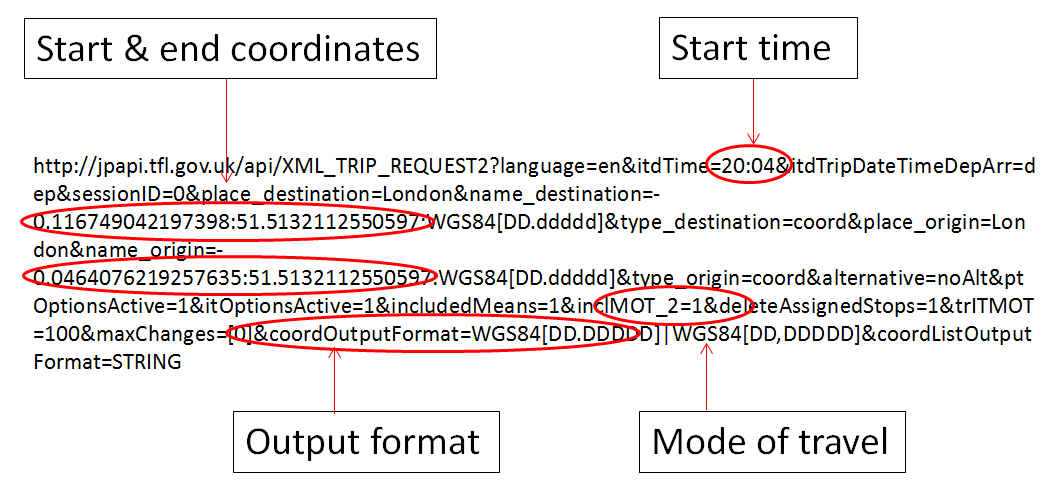
\includegraphics[scale=0.5]{tfl_api_call}
\caption{A 'call' to the TfL routing API}
\label{fig:tfl_api_call}
\end{figure}

This is submitted to the API using software of the users choice, code is written to parse the data that is returned (made into a format that the software can read), and then the results are stored and used as the user wishes.

A search of routing API services was therefore conducted, based upon the list detailed in the Wikipedia page 'Online Routers' (\url{http://wiki.openstreetmap.org/wiki/Routing/online_routers}) as well as an internet search of the term 'Online routing API'. A review of those considered suitable for this research is presented in table \ref{tab:api_summary_table}. A small handful of other APIs were dismissed before this stage as they were unsuitable for reasons such as geography (e.g. only covers Germany) or the API does not expose the route to the user (e.g. Bing Maps Directions plots the line onto a map, but does not give the actual data for storage).

\begin{landscape}
\begin{table}
    \hspace*{-.1cm}%
    \begin{tabular}{@{}| R{3.3cm} | R{3.2cm} | R{1.9cm} | R{3.2cm} | R{3.4cm} | R{4.5cm} |@{}}

    \hline

\textbf{API Service (coverage)} & \textbf{Available transport modes} & \textbf{Usage limits} & \textbf{Documentation} & \textbf{Simplicity of use} & \textbf{Customisation and notes} \\ \hline

Google Directions API (Worldwide) & Car, pedestrian, cycling, public transport & 750 per day (without license) & Provided, with many examples & Very simple to use & Limited. Parameters such as use of tolls, language of content, shortest or quickest. Public transport modes cannot be distinguished \\ \hline

OpenRouteService (Worldwide, but dependant on OSM data quality) & Car, pedestrian, cycling & Unlimited & In the form of a Wikipedia entry. Covers some examples but is not comprehensive. & Very simple & Limited. Road types, languages, zoom levels \\ \hline

Project OSRM (Open Source Routing Machine) (Worldwide, but dependant on OSM data quality) & Car & Unlimited & Basic instructions provided on GitHub & Very simple to use & Limited. Zoom level and output file type \\ \hline

Transport for London (Greater London) & Underground, overground, bus, train, tram, boat, cable---car, Docklands Light Railway & Unlimited (once registered) & Extremely comprehensive manual, but unclear in many places and often seemingly contradictory & Very difficult. Only simple examples are provided. So many parameters must be considered for a properly formed request & Fully customisable in almost every way. However it is limited to Greater London and does not alert when routes go outside. \\ \hline

MapQuest (Worldwide) & Car & Unlimited & Basic instructions provided on GitHub & Very simple to use & Limited. Zoom level and output file type \\ \hline

\end{tabular}\hspace*{-2cm}%%stop complaining
\caption{Summary of suitable routing APIs}
\label{tab:api_summary_table}
\vspace{-1cm}%%stop complaining
\end{table}
\end{landscape}

Each routing tool has advantages and disadvantages and it is therefore my expectation that a combination of these will need to be used depending on the specific use-case e.g. routes using the London Underground will need to use the TfL API.

%%%%%%%%%%%%%%%%%%%%%%%%%%%%%%%%%%%
%%% CMAQ-Urban
%%%%%%%%%%%%%%%%%%%%%%%%%%%%%%%%%%%

\section{CMAQ Urban}
\label{sec:cmaq_urban}

CMAQ (Community Multi-scale Air Quality model) is an ongoing open-source project, coordinated/led by the U.S. EPA Atmospheric Science Modelling Division. It is made up of a variety of software packages and processes for simulating air quality. To quote from their website, "CMAQ combines current knowledge in atmospheric science and air quality modeling with multi-processor computing techniques in an open-source framework to deliver fast, technically sound estimates of ozone, particulates, toxics, and acid deposition" (\cite{UnitedStatesEnvironmentalProtectionAgency2014}). The three main components are as follows (\cite{CMASCentre}):

\begin{enumerate}
\item A meteorological modelling system for the description of atmospheric states and motions
\item Emission models for man-made and natural emissions that are injected into the atmosphere
\item A chemistry-transport modelling system for simulation of the chemical transformation and fate
\end{enumerate}

ADMS-Urban is a separate air quality model which is distinctive as it is able to model a range of scales, from street to city, taking into account emissions sources such as traffic, industry and domestic sources. It incorporates advanced algorithms for the height-dependence of wind-speed, turbulence and stability to produce predictions. It also includes information on street canyons and mixing introduced by road traffic re-suspension  (\cite{CambridgeEnvironmentalResearchCounsultantsCERC2014a}).

The Environmental Research Group at King's College London, where the research within this report is taking place, have created a version of ADMS-Urban (KCL-Urban) which gives annual mean air quality predictions of NO, NO$_{2}$, O$_{3}$, PM$_{10}$ and PM$_{2.5}$ on a regular 20 m x 20 m grid. This is combined with a CMAQ regional scale model to create CMAQ-Urban which provides predictions of the same pollutants at the same scale on an hourly temporal resolution. The two models are equipped with similar capabilities in that KCL-Urban is quick to run and can provide details of the poor air quality sources at any location within it's domain. By combining these two ( CMAQ and KCL-Urban) the result is a model which is partly deterministic (uses fundamental physics and chemistry), but provides the same spatial detail as KCL-Urban. Importantly, it is therefore capable of predicting hourly concentrations (\cite{Beevers2013}). An example of the output of CMAQ-Urban is shown in Figures \ref{fig:kcl_urban_no2} and \ref{fig:cmaq_uk}.

\begin{figure}[H]
\centering
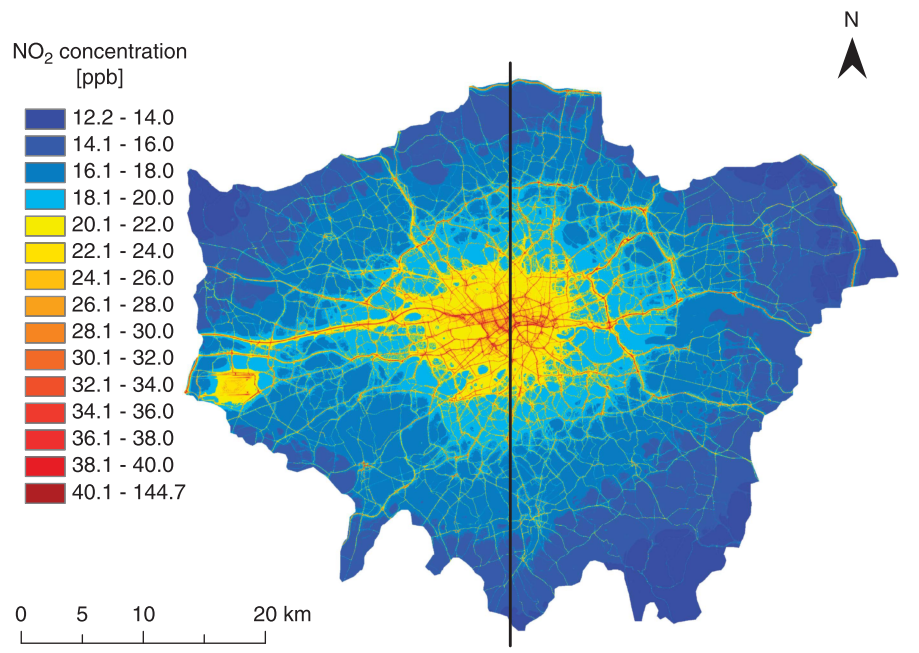
\includegraphics[scale=0.6]{kcl_urban_no2}
\caption{Annual mean NO$_{2}$ concentrations in London for the year 2008 predicted onto a regular grid of 20 m x 20 m using the KCLurban model.}
\label{fig:kcl_urban_no2}
\end{figure}

\begin{figure}[H]
\centering
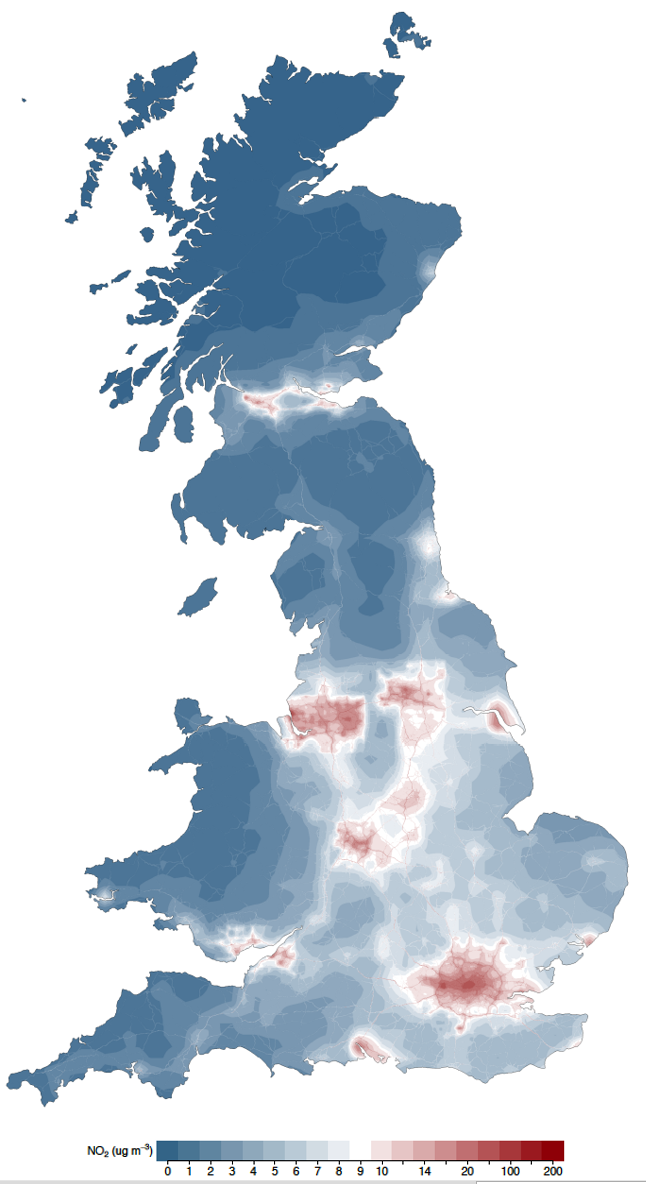
\includegraphics[scale=0.8]{cmaq_uk_v2}
\caption{An illustrative example of the domain covered by CMAQ-Urban}
\label{fig:cmaq_uk}
\end{figure}

CMAQ-urban was submitted to the  UK Model Intercomparison exercise run by the UK Government department DEFRA (\cite{Carslaw2013}), where it performed well against other urban and regional models with r values of 0.9 for NO$_{X}$ and NO$_{2}$, and 0.77 for PM$_{2.5}$.

For calculating exposure on a fine temporal (monthly-daily-hourly averages) and spatial scale (20 m x 20 m grids) the locations and time of individual subjects will be spatially joined with this model and then concentrations extracted from it.

%%%%%%%%%%%%%%%%%%%%%%%%%%%%%%%%%%%
%%% Interactive data visualisations
%%%%%%%%%%%%%%%%%%%%%%%%%%%%%%%%%%%

\section{Interactive data visualisations and animations}
\label{sec:interactivedata}

When it is desirable to produce maps of a higher quality, perhaps with interactive elements such as the user being able to click for more details or zoom in on areas of interest, the static maps that QGIS can produce as a PDF or similar are not suitable, and different tools are used to produce slippy maps (maps that can be dragged around using a mouse or other input device) with overlays of data. Figure \ref{fig:clear_streets} shows the website \url{www.clearstreet.org} which uses such a 'slippy' map and allows the viewer to zoom in or out on their area and examine the snow-plough activity.

\begin{figure}[H]
\centering
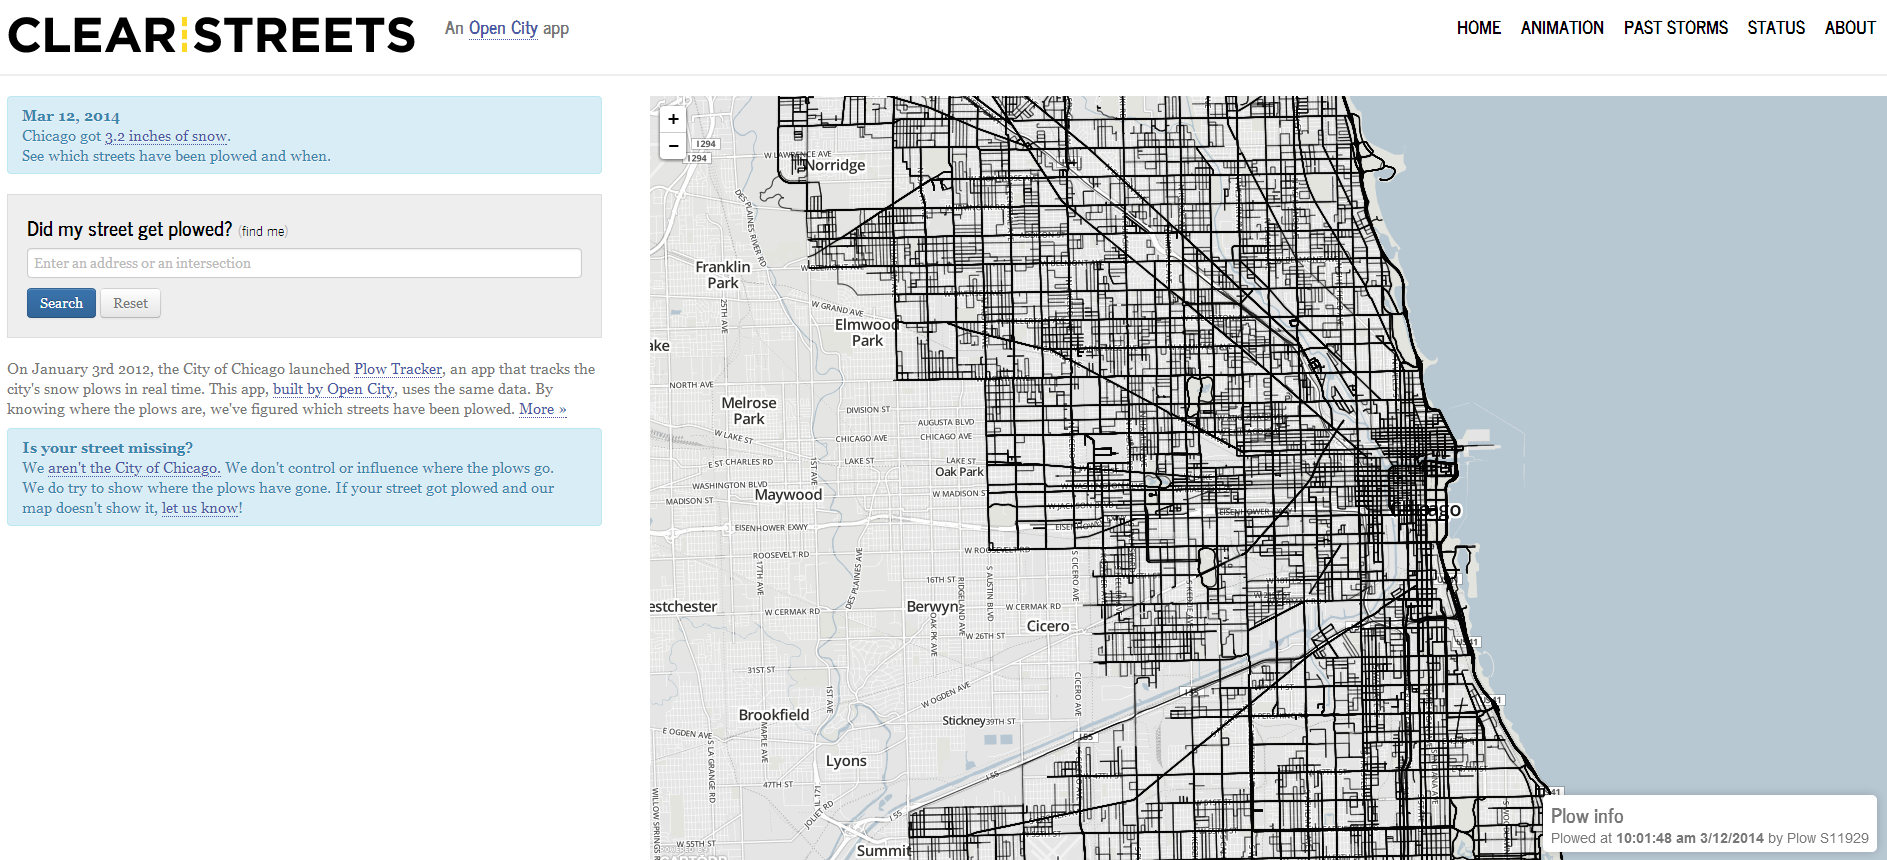
\includegraphics[scale=0.3]{clear_streets}
\caption{The clear streets website with a 'slippy' map}
\label{fig:clear_streets}
\end{figure}

Previously making maps of this type required specialist GIS and programming skills, and were almost exclusively made using the Google Maps API which allows embedding of the Google Maps data on your own webpage and with your own data added, however there has been a huge surge in mapping products over the last five to ten years as the profitability and usage of geographical data has become clear and commonplace respectively. As the field is rapidly evolving most books or review articles are out-of-date within weeks of publication, and therefore the following list of providers of global web-based slippy maps is taken from Wikipedia (\cite{wiki-maps-2014}):

\begin{itemize}
\item OpenStreetMap  (\url{http://www.openstreetmap.org/})
\item ArcGIS Online (Esri)  (\url{http://www.arcgis.com/home/webmap})
\item Google Maps \url{https://www.google.com/maps/})
\item Bing Maps (\url{http://www.bing.com/maps/})
\item MapQuest (\url{http://www.mapquest.com/})
\item WikiMapia (\url{http://wikimapia.org/})
\item HERE (\url{http://here.com/})
\item Mappy (\url{http://en.mappy.com/})
\item Yahoo! Maps (\url{https://maps.yahoo.com/})
\end{itemize}

Of this list the most popular and widely used are Google Maps and OpenStreetMap, however in following with the earlier stated aim of using FOSS tools, I decided to use OpenStreetMap background data for making online maps where needed in this research, due to it's community-made nature and lack of any restrictions on it's use or frequency of use.

To be able to use OpenStreetMap data as a background map with overlaps of data that has been produced during this research, further tools are needed. The two introduced below are both FOSS4G implementations of the javascript programming language and I intend to use them both as required, particularly for the later in this research where I explore novel visualisations and techniques for exposure and air quality data. 

\begin{itemize}
\item CartoDB.com (figure \ref{fig:cartodb_screen}): CartoDB is a cloud-based web-mapping, analysis and visualisation service. It allows storage of geographical data on their servers which can then be visualised on a map and published to a webpage. The advantages of CartoDB are the simplicity of producing professional looking maps with very little effort, however the amount of data that can be stored is limited without having to pay for additional storage. Despite this, for ad-hoc visualisations and/or ones that do not require a large amount of data to be displayed, this tool is very useful. CartoDB.com uses OpenStreetMap data as the background for the maps that it serves to the users and can be easily customised.
\item Leaflet.js: Leaflet prides itself as a lightweight javascript library which displays OpenStreetMap data. By lightweight the community developers emphasise the very small amount of coding and expertise that is required to produce a map. Adding data and creating visualisations on top of the map is then of moderate difficulty. The main difference between CartoDB and Leaflet is that leaflet does not store the data, the webpage is coded so that the data is fed to it from another source such as an API or indeed a CSV file or similar which is stored on the same server as the map-coding itself. This has the advantage of there being no data-storage limits as the developer is responsible for the data themselves, however the knowledge and skills required to put the data onto the map are more advanced than that of using CartoDB.
\end{itemize}

\begin{figure}[H]
\centering
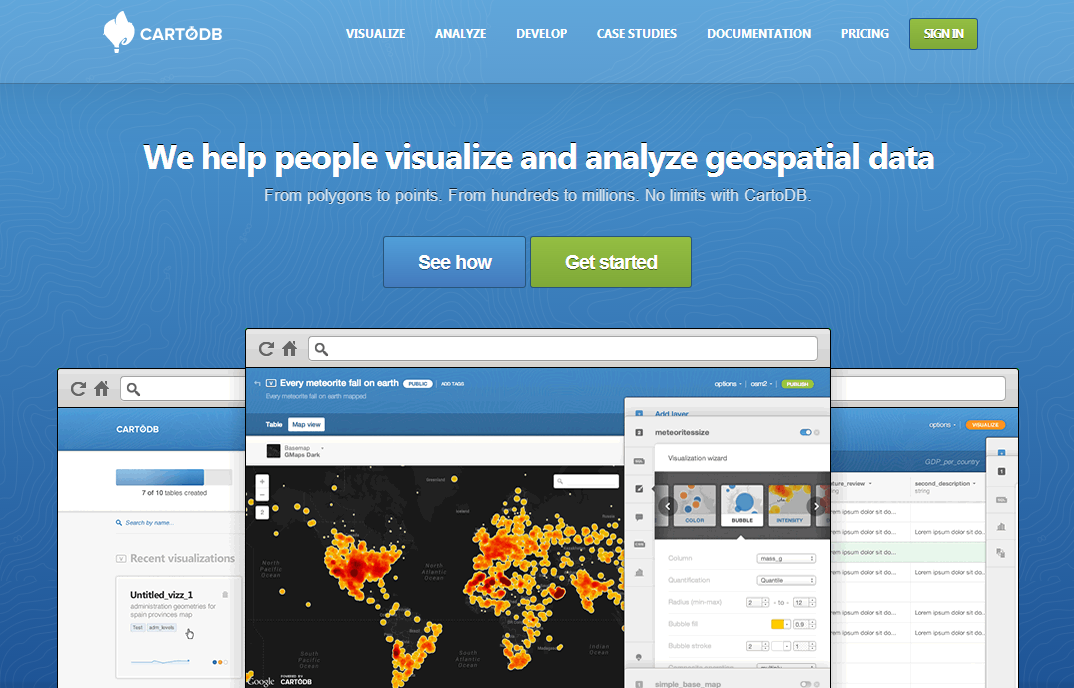
\includegraphics[scale=0.5]{cartodb_screen}
\caption{The CartoDB data visualisation platform}
\label{fig:cartodb_screen}
\end{figure}

When outputs of this research are required that are not suitable for a map, then I will make graphs and charts using the plotting functionality of the FOSS 'R' project (\cite{RFoundationforStatisticalComputing2014}). One of the benefits of using R is that it can be easily connected to the PostgreSQL RDMS that was chosen earlier, and then statistical analysis and publication-quality plots can be produced with relative ease and a few lines of coding.  For interactive or web-based charts and graphs the D3 javascript library developed by Mike Bostock will instead be used (\cite{Bostock:2011:DDD:2068462.2068631}) for similar reasons - it is free, open-source, and there is a large community of developers actively using it which gives a great deal of inspiration and examples to base future work on e.g. \url{https://github.com/mbostock/d3/wiki/Gallery}.

\chapter{Modelling Londoners movements}
\label{chap:the_ltdsx}
%%%%%%%%%%%%%%%%%%%%%%%%%%%%%%%%%%%%%%%%%%%%%%%%%%%%%%%%%%%%%%%%%%%%%%%%%%%%%%%%%%%
\section{Aim}
\label{sec:1aim}
%%%%%%%%%%%%%%%%%%%%%%%%%%%%%%%%%%%%%%%%%%%%%%%%%%%%%%%%%%%%%%%%%%%%%%%%%%%%%%%%%%%

Create a model of Londoners daily movements based upon the London Transport Demand Survey

%%%%%%%%%%%%%%%%%%%%%%%%%%%%%%%%%%%%%%%%%%%%%%%%%%%%%%%%%%%%%%%%%%%%%%%%%%%%%%%%%%%
\section{Objectives}
\label{sec:1objectives}
%%%%%%%%%%%%%%%%%%%%%%%%%%%%%%%%%%%%%%%%%%%%%%%%%%%%%%%%%%%%%%%%%%%%%%%%%%%%%%%%%%%

\begin{itemize}
\item Explore the LTDS dataset and identify key data
\item Move data from local Microsoft Access database into a PostgreSQL + PostGIS database
\item Clean data
\item Complete modal specific routing (interrogation, querying, storage) between origin and destinations
\item Quality check the routing results and do further data cleaning
\item Create and populate final dynamic location database table
\item Analysis of results
\end{itemize}

%%%%%%%%%%%%%%%%%%%%%%%%%%%%%%%%%%%%%%%%%%%%%%%%%%%%%%%%%%%%%%%%%%%%%%%%%%%%%%%%%%%
\section{Background}
\label{sec:1_background}

As was heavily discussed in Section \ref{sec:staticexposurehealth} many air quality exposure studies do not consider the movements of the subjects and/or to varying degrees other factors such as the temporal fluctuations in pollutant concentrations and levels of infiltration into micro-environments such as the home. The aim of this chapter was to process and characterise the LTDS prior to application to the hybrid exposure model. 

This was achieved by using the methods outlined in Sections \ref{sec:spatialdatabases} (Spatial databases), \ref{sec:gis} (GIS) and \ref{sec:routing} (Routing), and reconstructing the time-space location of the population of London on a minute-by-minute basis, using the LTDS dataset. This allowed interrogation of the data and such questions to be answered as; how much time do people spend indoors each day, and is there ethnic bias in the distance that people travel to work? To demonstrate the capacity of the model/dataset visualisations/maps of peoples routes were created and summary graphs of interesting information.

%%%%%%%%%%%%%%%%%%%%%%%%%%%%%%%%%
\section{Methods}
\label{sec:1_methods}

\subsection{Data Processing}
\label{sec:reconstruction_data_processing}

The LTDS comprised of around 58 tables of data stored in an Microsoft Access database. The majority of these tables were 'look-up' tables that store information that can be linked too from other tables e.g. the Stages table described the stages of trips that the subjects made, and had a column for transport mode which simply contains integers in the range 1-26. These integers needed cross-referencing against the Mode table to ascertain their meaning (1 = walk, 3 = car etc). This allows for more efficient storage of data, but made gaining a full understanding of the dataset and how tables linked together a lenghty process. The four key tables that were required were (as briefly discussed in Section \ref{sec:the_ltds}) the Household, Person, Trip and Stage tables. Within each table there were columns that were more or less useful than others.  Table \ref{tab:key_ltds_fields} below lists some of the more important and useful ones:

\newpage

\begin{center}
\begin{table}[h!]
    \begin{tabular}{ | p{2.2cm} | p{12cm} |}
    \hline
    \textbf{Table} & \textbf{Key fields} \\ \hline
    \multirow{2}{*}{Household} & hhid: household id \\
     & hhaboro: Household Borough \\
     & htdate: Date house survey refers too \\
     & hincomeei: Household income \\
     & hhose and hhosn: easting and northing of household \\ 
     & householddatatime: This column was created and populated with a full time-stamp \\ \hline
   \multirow{2}{*}{Person} & phid: Person id \\
     & phid: Household id of person \\
     & ppiwt: Expansion factor of person \\
     & psexi: Person gender \\
     & pagei: Person age \\
     & pegroup: Person ethnic group \\
     & pegroup: Person ethnic group \\
     & pseg: Person socio-economic group \\
     & pnotrips: Number of trips person takes in survey 24 hours \\ \hline
     \multirow{2}{*}{Trip} & ttid: Trip id \\
     & tpid: id of person doing the trip \\
     & tstagesn: Number of stages in the trip  \\
     & tdpurp: Destination purpose of trip \\
     & tstime: Trip start time \\
     & tetime: Trip end time \\
     & toose and toosn: Trip origin (OSGB36 Easting and Northing) \\
     & tdose and tdosn: Trip destination (OSGB36 Easting and Northing) \\
     & tdurn: Duration of trip \\ 
     & departuretime: This column was created and populated with a full time--stamp of the trip departure time \\
     & arrivaltime: This column was created and populated with a full time--stamp of the trip arrival time \\ \hline
    \multirow{2}{*}{Stage} & ssid: Stage id \\
     & stid: Trip id \\
     & smode5y: Stage mode of transport \\
     & soose and soosn: Stage origin (OSGB36 Easting and Northing) \\
     & sdose and sdosn: Stage destination (OSGB36 Easting and Northing) \\
     & sdurn: Duration of trip (minutes) \\
     & stagedeparturetime: This column was created and populated with a full time--stamp of the stage departure time \\
     & stagearrivaltime: This column was created and populated with a full time--stamp of the stage arrival time \\ \hline
    \end{tabular}
    \caption{Key LTDS fields}
    \label{tab:key_ltds_fields}
\end{table}
\end{center}

The tables listed above were exported as CSV files and then imported into a PostgreSQL installation on a virtual Ubuntu machine. PostGIS was then added to the PostgreSQL installation. SQL scripts were ran to create full time-stamp columns in the Household, Trip and Stage tables rather than use the format that the data was stored in e.g. dates were stored in the Household table in the form '20060221' (meaning 2006-02-21) and times in the Trips table as '730' (meaning 07:30) which made performing temporal queries on them difficult. Further complications arose in the Trips and Stages tables as the survey period begins and ends at 4am (or once the persons final trip was completed). So times in the Trips table showed as, for instance ,'300' which meant 3am, however that actually meant 3am on the morning of the day after the survey date, rather than the survey date itself. Another factor was that the stages table did not contain any stage departure times or stage arrival times, only the duration of each stage. Therefore the stages table needed cross-referencing against the trip table and then summing incrementally by stage id in order to calculate the correct stage departure and arrival times (and then extensively checking).

\subsection{Data cleaning}
\label{sec:reconstruction_data_cleaning}

Data cleaning was required throughout the methods, however is briefly mentioned here. A number of different processes were required, a few of which are listed as bullet-points below. It should be noted that an early decision was taken whereby if any data linked to a Person was clearly incorrect, or not recorded properly, then that person was removed from the dataset entirely (by creation of a column in the Person table titled 'badflag' and then entering the reason the person was removed). For example if a person had a stage which started 15 minutes before the next noted stage began, that person was removed rather than just a correction of the data (in this case because it would be difficult to know stage which to correct). Removal of records from the dataset occurred in the following situations:

\begin{itemize}
\item Trip start and end times were mis-aligned
\item Stage start and end times were mis-aligned
\item Stage transport mode was missing or refused
\item Key demographic data was missing or refused
\item Stage start and end locations were mis-aligned with the next or previous trip by greater than 80 metres
\item LTDS respondent did not live in London (the survey stretches just beyond the London Borough boundary)
\item Location of stage start or stage end were missing.
\item Transport mode was not available via a known API e.g. Plane or a bus journey outside of London
\end{itemize}

To ensure that removal of subjects from the dataset had not compromised the overall structure and statistical strength of the data (and therefore made using the weighting factors to scale the data unsuitable), t-test and Wilcoxon–Mann–Whitney tests were performed to compare the original data, and this subset of data. No statistical significance was found when comparing age, Borough of residence, ethnicity, income, sex, distances travelled each day, or the amount of time in transport. The final dataset to be used was therefore judged as suitable for purpose.

\subsection{Mode-specific routing}
\label{sec:reconstruction_mode_routing}

To calculate the locations of the subjects while they were travelling between locations the stages table of the LTDS was used, specifically the start easting and northing, the destination easting and northing, the transport mode, and the stage departure time (if allowed as an input by the API). These columns were extracted from the database directly into R using the RPostgreSQL extension and stored in an R dataframe. These details were then formed into URL requests and sent to the routing APIs by R. A small extract of the large XML file that is received in response to a request to the TfL Journey Planner API is shown in Figure \ref{fig:tfl_response_example}. This was parsed using the RJSONIO and XML packages, and the route between the two locations extracted and stored (and then decoded in the case of Google). The route was then formed into a linestring data type (which PostGIS can store as a spatial object) and entered back into the database as the route taken between the coordinates in an extra column called 'the\textunderscore geom'.

\begin{figure}[H]
\centering
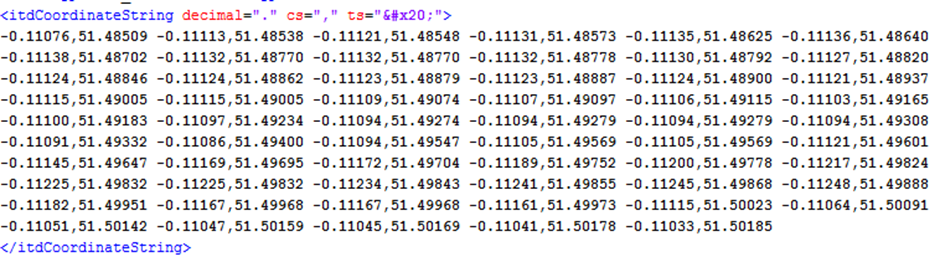
\includegraphics[scale=0.9]{tfl_response_example}
\caption{An example of an XML response from the TfL API}
\label{fig:tfl_response_example}
\end{figure}

Due to restrictions on usage limits, and the modes of transport that each API has available, different APIs were used for each transport mode in the LTDS (see Table \ref{tab:api_transport_modes}). Pre-processing was required to simplify the transport modes before this, for example the LTDS contains transport modes such as 'Car (passenger)', 'Taxi', 'Van (driver)', 'Van (passenger)' and 'Motorcycle (driver)' which were combined to the mode of 'car' given that the likely routes would be the same (and more importantly that the API did not have the ability to distinguish between them as an input).

\begin{table}[H]
\hspace*{-.1cm}%
    \begin{tabular}{@{} | R{5cm} | R{8cm} |@{}}
    \hline 
     \bfseries{LTDS Transport Mode} & \bfseries{API} \\ \hline
     Walking & OpenRouteService (\url{www.openrouteservice.org}) \\ \hline
    Cycling & Google Directions \\ \hline
    Train, Overground, Underground, Docklands Light Railway, Bus & Transport for London Journey Planner \\ \hline
    Car & Project OSRM API (\url{www.project-osrm.org}) \\ \hline
    \end{tabular}\hspace*{-2cm}%%stop complaining
\caption{APIs used for each LTDS transport mode}
\label{tab:api_transport_modes}

\end{table}

The cleaned data contained 45,079 people, who took 98,770 trips during the day of the survey. Each trip consisted of multiple stages that needed routing independently, totally 340,754. These 340,000 routes were stored as linestrings in the PostGIS database next to the id (ssid) of the stage.

\subsection{Quality checking}
\label{sec:reconstruction_quality_checking}

Spatial cleaning of the routes was now performed. This is discussed earlier in Section \ref{sec:reconstruction_data_cleaning}. It primarily consisted of error-checking of the routes that had been obtained from the APIs by making visualisation of the transport modes to manually identify large errors e.g. were there any tube journeys recorded as being in Scotland, or a taxi journey accross the Irish sea. The results of the underground and Docklands Light Railway (DLR) routing are shown in \ref{fig:underground_routing} below.

\begin{landscape}

\begin{figure}[H]
\centering
\frame{\includegraphics[scale=0.65]{underground_routing}}
\caption{A visual check that the underground routes actually are on the underground lines}
\label{fig:underground_routing}
\end{figure}

\end{landscape}

\subsection{Data manipulation}
\label{sec:reconstruction_data_manipulation}

A 'base table' for each subject in the cleaned and routed LTDS data (45,079) was now created (and named the hybrid\textunderscore location table). This table contained four columns, Person ID (ppid), Time (pointtime), Mode (mode) and Location (thegeom). A blank row for every minute of the subjects 24 hours was created (45,079 subjects, multiplied by 24 hours, multiplied by 60 minutes). The table was then populated with data from the Stage table, by taking the line-strings of each route and splitting them into minute-by-minute interval points using bespoke spatial interpolation SQL scripts, and then matching those points to the correct time in the new table. The mode and id of the stage were also copied over for ease of future reference. A graphic which attempts to demonstrate the premis behind the spatial interpolation method is shown below in \ref{fig:spatial_interpolation_example}.

\begin{figure}[H]
\centering
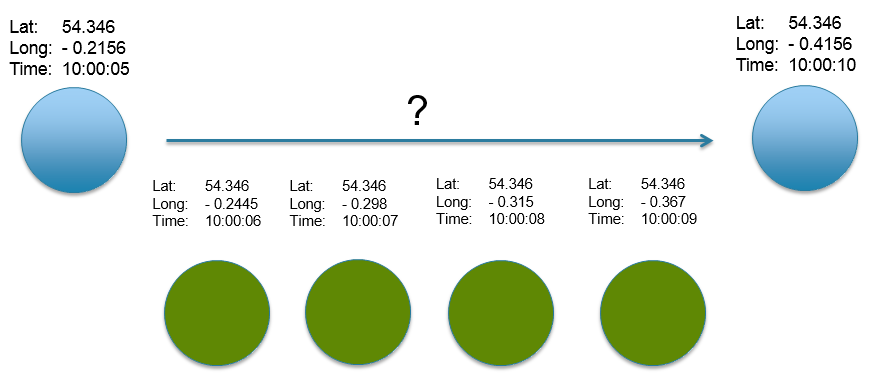
\includegraphics[scale=0.6]{spatial_interpolation_example}
\caption{The time and location between two known locations and times were calculated using custom-made SQL scripts and the spatial functions of PostGIS}
\label{fig:spatial_interpolation_example}
\end{figure}

Inbetween Trips subjects were presumed to be stationary and indoors at the final point recorded of the previous trip. At the start and end of days subjects locations were presumed to be the starting point of their first trip, and the ending location of their last trip respectively (and again, indoors). By doing this the location of the 45,079 people were calculated and stored on a minute-by-minute basis for 24 hours. An extract of the final table is shown below in \ref{fig:hybrid_location_table} (for reference mode 0 = indoors, 1 = walking, 3 = car).

\begin{figure}[H]
\centering
\frame{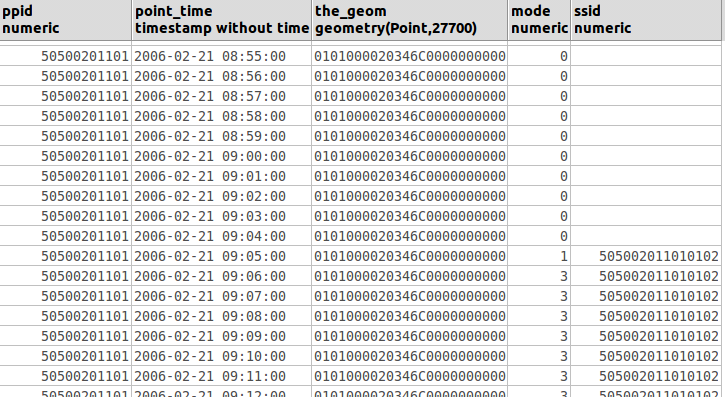
\includegraphics[scale=0.6]{hybrid_location_table}}
\caption{An example of data and structure in the hybrid location table}
\label{fig:hybrid_location_table}
\end{figure}

%%%%%%%%%%%%%%%%%%%%%%%%%%%%%%%%%
\section{Results}
\label{sec:reconstruction_results}

The hybrid location table was used to examine the movements of the subjects of the LTDS on a fine temporal and spatial scale. The data was explored to better understand the detail available, to check that it was suitable for use as the basis of a dynamic exposure model, and to see whether there were any interesting results already present before air quality was considered.

\subsection{Visual inspection of individuals}
\label{sec:visual_inspection_of_individuals}

Before starting to summarise data and look for patterns in large groups of people, Figures \ref{fig:routed_results_example} and \ref{fig:routed_results_example2} were created and show the results of two randomly selected individuals from the dataset. The first (\ref{fig:routed_results_example}) shows a fairly simple reconstructed day. The Person made two car journeys around the local neighbourhood, as well as one walking trip to a few streets away. Other than visiting those three local locations, they spent their time at home. The second (\ref{fig:routed_results_example2}) shows a much more complicated picture. The individual lives near Norbiton. In the morning they walked to Norbiton station, took a train to Waterloo, and then caught a bus to Clerkenwell (presumably for work). At lunchtime they walked around the local neighbourhood (buying lunch?). At 20:13 they took a taxi back to Waterloo, where they got a train back to Norbiton, and walked home from the station to their house.

\begin{landscape}

\begin{figure}[H]
\centering
\frame{\includegraphics[scale=0.65]{routed_results_example}}
\caption{Example one of the reconstruction of a subjects day}
\label{fig:routed_results_example}
\end{figure}

\newpage

\begin{figure}[H]
\centering
\frame{\includegraphics[scale=0.65]{routed_results_example2}}
\caption{Example two of the reconstruction of a subjects day}
\label{fig:routed_results_example2}
\end{figure}

\end{landscape}

\subsection{Journey start and end times}
\label{sec:journey_start_and_end_times}

By grouping the start times of the stages by hour, and then summarising by the number of stages within that hour, a histogram of journey start times was created (Figure \ref{fig:when_people_start_trips}).

\begin{figure}[H]
\centering
\includegraphics[scale=0.48]{when_people_start_trips}
\caption{Histogram of when the population of London start trips}
\label{fig:when_people_start_trips}
\end{figure}

A similar method was also used for the ending times (Figure \ref{fig:when_people_end_trips}).

\begin{figure}[H]
\centering
\includegraphics[scale=0.48]{when_people_end_trips}
\caption{Histogram of when the population of London end trips}
\label{fig:when_people_end_trips}
\end{figure}

Figures \ref{fig:when_people_start_trips} and \ref{fig:when_people_end_trips} show peaks of travel around peak travel times that might be expected in the morning and evening rush hours, however it is interesting to note that considerable travel occurs during the day (although at this stage the data is not split by specific days, so this may be influenced by travel on a Saturday and Sunday). It was also interesting to see how trips during the evening (4pm-8pm) are much more dispersed than in the morning, suggesting that people tend to leave work over a longer time-frame than when they start work. 

\subsection{Journey distances by sex}
\label{sec:journey_distances_by_sex}

By summing the total distance travelled by each person over 24 hours, and then grouping by gender, graph \ref{fig:mean_distance_by_sex} shows differences in total travel distance.

\begin{figure}[H]
\centering
\includegraphics[scale=0.5]{mean_distance_by_sex}
\caption{Boxplot of distances travelled, by gender (outliers \textgreater 100 km omitted for clarity, red line links each mean)}
\label{fig:mean_distance_by_sex}
\end{figure}

Although the difference was not huge (Male mean of 18.28 km, Female mean of 13.89 km), there was a significant difference (using a t-test) between the kilometres that each gender travels in a day. Whether this is because women stay at home more than me, or whether the journeys that men are required to do during their day take them further was not clear (but could be investigated further as the dataset contains a great deal of contextual information).

\subsection{Journey distances by income}
\label{sec:journey_distances_by_income}

A similar method was then used but the demographic of household income was used as the variable to be considered rather than gender (individual-level income variables were unfortunately not collected). The result is shown in Figure \ref{fig:mean_distance_by_income}.

\begin{figure}[H]
\centering
\includegraphics[scale=0.5]{mean_distance_by_income}
\caption{Boxplot of distances travelled by income group  (outliers \textgreater 100 km omitted for clarity, red line links each mean)}
\label{fig:mean_distance_by_income}
\end{figure}

Interestingly the dataset showned that subjects that live in households with a higher income actually travel further than households with a lower income level (albeit with a levelling off and even slight dip around the \textsterling75,000 mark).

\subsection{Journey distances by age group}
\label{sec:journey_distances_by_age_group}

Distance of travel by age group was now plotted in Figure \ref{fig:mean_distance_by_age}.

\begin{landscape}

\begin{figure}[H]
\centering
\includegraphics[scale=0.7]{mean_distance_by_age}
\caption{Mean distances travelled by age group (outliers \textgreater 100 km omitted for clarity, red line links each mean)}
\label{fig:mean_distance_by_age}
\end{figure}

\end{landscape}

Figure \ref{fig:mean_distance_by_age} showed a clear rise in the distance that people travel each day as they get into their late teens, which then becomes fairly steady until mid-50s at which point the distances start to decline again. That said, a clear cut-off was not visible. The gradient of the slops between 60 and 90 is much more steady that at the other end of the age range, perhaps showing that the ages that people retire are more dispersed than the ages at which people start work.

\subsection{Journey distances by Borough of residence}
\label{sec:journey_distances_by_borough_of_residence}

The distances that the people of London travel, depending on their Borough of residence, was now considered. The centre of London was defined (the monument outside of Charing Cross station) and then the distance between this point and the centroid of each London Borough was calculated (Figure \ref{fig:borough_centroids}). Figure \ref{fig:mean_distance_by_borough} was then created, with the Boroughs ordered by this distance metric i.e. the centroid of the City of London is the closest Borough centroid to Charing Cross, so was plotted first. This ordering was undertaken as I theorised that individuals living nearer the centre of London would spend less time travelling than those in outer London.

\begin{figure}[H]
\centering
\frame{\includegraphics[scale=0.5]{borough_centroids}}
\caption{Calculating Borough centroids to Charing Cross}
\label{fig:borough_centroids}
\end{figure}

\begin{landscape}

\begin{figure}[H]
\centering
\includegraphics[scale=0.7]{mean_distance_by_borough}
\caption{Mean distances travelled by Borough of residence}
\label{fig:mean_distance_by_borough}
\end{figure}

\end{landscape}

There did not appear to be any clear pattern between where people live and the distance that they travel each day. As the Boroughs were plotted in order, if it was true that people living in outer London Boroughs travel more, then the medians and means of the graph should rise from left (closest to centre of London) to right (furthest from centre of London). The Borough with the lowest mean was actually found to be Greenwich, perhaps reflecting that the people who live in Greenwich tend to work more locally (this could be investigated using the dataset). The boroughs with the highest mean travelling distance were Havering, Richmond and Merton.

\subsection{Transport mode choice by age group}
\label{sec:transport_mode_choice_by_age_group}

Focusing now on transport mode choice, the percentage of time that each person spends within each micro-environment, namely bus, car, cycling, train, underground and walking, was calculated. The indoors environment was found to be very dominant i.e. people spent most of their days indoors. For clarity of visualisation, the indoor environment was removed, and the remaining ones plotted by age bracket (Figure \ref{fig:age_barplots_time_transport}).

\begin{figure}[H]
\centering
\includegraphics[scale=0.7]{age_barplots_time_transport}
\caption{Percent of typical day using transport modes by income bracket}
\label{fig:age_barplots_time_transport}
\end{figure}

This graph agrees well with Figure \ref{fig:mean_distance_by_age} (travel distances by age group) which showed a bell-curve like distribution, with a leaning towards the upper age groups. Additionally however Figure \ref{fig:age_barplots_time_transport} shows how use of transport modes changes with age. Except for the 0--10 age group, bus transport is used the same amount by all ages. Walking has a similar pattern, being used frequently by people even up to the ages of 80 and above. Cycling is popular with the 20 to 60 year old's, but then hardly used by people older than that. The underground results are interesting in that it is almost never used by anyone in the 0-10 age bracket, or the 80+ age bracket. Despite free travel being granted to people in those age groups.

\subsection{Time near residence}
\label{sec:time_near_residence}

One of the main motivations behind this research was to examine where people spend time, and therefore accumulate their exposure, and whether using address or postcodes (or dynamic methods) for exposure assessment was valid. To examine this, a 1 km buffer was created around each residents recorded residential address (example shown in Figure \ref{fig:one_km_buffer_house}).

\begin{figure}[H]
\centering
\includegraphics[scale=0.6]{one_km_buffer_house}
\caption{Example of a 1 km buffer around residential address}
\label{fig:one_km_buffer_house}
\end{figure}

Then the percent of time that each occupant of each house spends within that buffer was calculated. The results are shown in Figure \ref{fig:time_with_one_km_home_by_age}.

\begin{landscape}

\begin{figure}[H]
\centering
\includegraphics[scale=0.9]{time_with_one_km_home_by_age}
\caption{Boxplot of percent of time within 1 km of home address, means shown by red line}
\label{fig:time_with_one_km_home_by_age}
\end{figure}

\end{landscape}

Figure \ref{fig:time_with_one_km_home_by_age} shows an interesting pattern of time spent within subjects local neighbourhoods varying by age group. Considering the mean line (red), time spent at home hovers between the 70\% and 80\% mark with some small variation up and down between the ages of 5 and 60. From age 60 onwards the time spent within the local neighbourhood steadily increases to 90\% by age 70, and mid 90s from there onwards (with a sudden dip in the 98 and 99 year olds, however this seems likely to be due to small numbers of subjects of this age who happened to be quite active on the day of the survey).

For illustrative purposes three simple animations of the data--set were made. The first two using the QGIS TimeManager plug-in, and the third using javascript. They can be viewed online at the following URLs:

\begin{itemize}
\item A webpage with an interactive slider, whereby the user can view the time--activity points of the trips the subjects of the LTDS make, on a minute by minute basis, with the points colour-coded according to the mode at that point--time:
\begin{itemize}
\item \url{http://www.londonair.org.uk/research/dynamic_london/mode_animation.html}
\end{itemize}
\item An animated GIF file of the movements of the LTDS, clipped to show specifically London
\begin{itemize}
\item \url{http://www.londonair.org.uk/research/ltds_uk/traffic_london.gif}
\end{itemize}
\item An animated GIF file of the movements of the LTDS, showing the whole of the UK
\begin{itemize}
\item \url{http://www.londonair.org.uk/research/ltds_uk/traffic_uk.gif}
\end{itemize}
\end{itemize}

These illustrations allow a much better understanding of the data--set than was possible before. Instead of rows of an database, the data can be viewed and understood. When used in presentations to colleagues and external stakeholders (such as the TfL staff who collect the LTDS data), it was particularly useful in helping them become more familiar with the results of the process. Particularly interesting to note in the animations is the spatial distribution of the LTDS subjects, with their movements on the day of the survey clearly not limited to the geographical area of London (and thus justifying the need for a UK-wide CMAQ model of air quality concentrations). Also the number of people who travel from London to outside of London for work or otherwise.

%%%%%%%%%%%%%%%%%%%%%%%%%%%%%%%%%
\section{Discussion}
\label{sec:1Discussion}

Generating or manipulating the LTDS with the methods and tools discussed in this chapter proved complicated, particularly in writing the SQL and R scripts to interrogate the APIs, and then the spatial and temporal interpolation techniques to re-define the data in the resolution required. However having initially attempted to build custom transport networks using PostGIS and PgRouting (the PostgreSQL extensions), the methods attempted were much more productive in that they allowed a far higher percentage of routes to be solved, and with much higher accuracy. 

The dataset that has been produced is, to my knowledge, unparalleled in this area of study. Few studies have produced similar datasets, a notable one being \cite{Dhondt2012} and their 5 million subjects in the 'FEATHERS' dataset, however the temporal resolution of that model was only hourly and the spatial resolution down to 16 km by 16 km zones of Flanders (Belgium) rather than exact coordinates. Conversely, it could be argued that the hybrid\textunderscore location table actually be more highly resolved that it is. Time intervals of one-minute were chosen for convenience, when 30 seconds or even 1 second could have been used. However this seemed the most sensible choice on the basis that the dataset is already very large. Further research to assess the impact of perhaps changing to 30 second intervals could be worthwhile. The linked demographic data to the people and households of this data was also very useful in examining travelling patterns and mobility by different characteristics, which has been done in many studies before however normally by using crude measures such as euclidean distances between households and recorded workplaces, rather than by using routing solutions.

The limitations of this approach include the lack of finely-detailed control over the routing process and solution. Whilst most of the APIs allowed for different transport modes to be selected, and some of them give options such as 'avoid major roads', they do not allow cost-factors to be dynamically assigned to roads or for the network to be manipulated such as removing specific routes from the choices available. Whilst not an issue at this stage of this research, a situation can be envisaged whereby low exposure routing would be desirable, and this will prove difficult. Similarly, there is currently no way of validating the routes that were chosen by the subjects, as being representative of the actual routes taken. For some transport modes this seems less of a worry than for others. A subject taking a tube from London Bridge to Elephant and Castle for example has very little choice of their route (without significantly adding time to their journey), and much would be the same for other journeys using public transport. Private modes such as driving and walking would be less certain, however the time taken for the route matches the time in the LTDS, so whilst small detours are possible, large detours are unlikely.

The way that time inbetween trips is considered might be leading to an over-estimation of the amount of time that subjects spend indoors each day. This is because when subjects finish trips the model presumes that they are then inside until the next trip begins. Time spent not travelling but in outdoor spaces, is therefore neglected (for example in a park). Intersecting an Ordnance Survey land-use map with the dataset could lead to improvements in this area of the model. Further efforts could also be made to 'recover' discarded data which was removed in the data-cleaning process, for example subjects with miss-aligned trip start and end times were removed, but further investigation may have been able to resolve these issues.

Going forward, this dataset will now be referred to for simplicity as the LTDS-Expanded dataset, or the LTDS-X for short.  Specifically, the dataset created (expanded) by processing of the original LTDS data through routing algorithms and GIS.

%%%%%%%%%%%%%%%%%%%%%%%%%%%%%%%%%
\section{Conclusions}
\label{sec:1conclusions}

The aim of this research was to process and characterise the LTDS to create a new data--set that can be used as an input for a hybrid exposure model. Spatially-enabled databases with custom scripts were wrote to do this, R was used as an interface with various APIs, and the 'hybrid\textunderscore location' table was created successfully. Extensive quality checking and data cleaning was undertaken. The final data-set allows interrogation of the daily activities of 6.8 million people in London, which can be interrogated on a fine spatial and temporal detail, aswell as by various demographics. The main findings from this data--set were as follows:

\begin{itemize}
\item There are peaks in travel between 8am and 10am in the morning, and between 5pm and 6pm in the evening (As would be expected), however substantial travel also occurs between those hours.
\item Men travel more each day than women (mean of 18.28 km, compared to women with 13.89 km).
\item Households with a higher average annual income, are inhabited by people who travel more than households with a lower average annual income.
\item The distances that people travel each day increases as they get older, peaking around the ages of 38-42. It then steadily declines, however much more gradually than it rose. By late 80s, people travel very little.
\item There appears to be no pattern to where people live compared to the distances they travel each day
\item The amount of time that people spend in transport each day peaks in the 30-50 age categories.
\item Car use is the most popular form of transport amongst all age groups over 20 (until that point walking is the most popular). Walking is the second most popular, followed by the London Underground.
\item People over 80 rarely use the London Underground.
\item The amount of time that people spend within 1 km of their home, when analysed by age group, has a similar but slightly different pattern as the distance that people travel. Between the ages of 5 and 20, the mean is around 77\%, which then drops to the low 70\% mark for people aged 20 to late 50s. From 60 onwards, the time at home gradually increases up to high 80s.
\end{itemize}

This initial exploration and validation of the key characteristics of the data were important to confirm that it was suitable for use in further research. It will now be used as the main input for a hybrid exposure model to estimate subjects exposure to air pollution. 

\chapter{Dynamic exposure modelling}
\label{chap:the_lhem}
\section{Background}
\label{sec:exposure_background}

Chapter One focused on processing, checking and exploring the spatial data that was created from the LTDS, leading to the LTDS-X. The daily journeys of around 45,000 people were recreated on a fine spatial and temporal scale from survey data. This data-set was created to allow investigation of exposure in urban environments, and also miss-classification, as described in Section \ref{sec:dynamicexposurehealth}, namely the differences between assigning someone a static exposure value based on their home location, postcode, nearest monitoring site or otherwise, compared with a model which considers all the micro-environments and varying concentrations during the subjects daily movements.

The thrust of this chapter will therefore be to link the LTDS-X dataset to the CMAQ-Urban dataset (described in \ref{sec:cmaq_urban}), and then to undertake micro-environmental modelling for when the subjects are indoors and for when they are in transport. The completed model of exposure is henceforth referred to as the London Hybrid Exposure Model or LHEM. The LHEM will then be used to explore exposure variations within the subjects, to attempt to identify and understand any patterns, and to consider exposure missclassification that may be occurring using standard exposure methods. Potential policy uses of the LHEM, and ways in which it might be useful to the general public, are then discussed.

%%%%%%%%%%%%%%%%%%%%%%%%%%%%%%%%%%%%%%%%%%%%%%%%%%%%%%%%%%%%%%%%%%%%%%%%%%%%%
\section{Methods}
\label{sec:exposure_methods}
%%%%%%%%%%%%%%%%%%%%%%%%%%%%%%%%%%%%%%%%%%%%%%%%%%%%%%%%%%%%%%%%%%%%%%%%%%%%%

In order to calculate the 'static' exposure estimates which will be compared to the LHEM estimates, a number of input data-sets and methods/processes needed to be completed. They are now listed and explained below, with the methods and input data-sets grouped by the final dataset under construction.

%%%%%%%%%%%%%%%%%%%%%%
    \subsection{Running the London Hybrid Exposure Model}
    \label{sec:running_the_lhem}
%%%%%%%%%%%%%%%%%%%%%%

        \subsubsection{Linking LTDS-X to outdoor concentrations}
        \label{sec:linking_ltdsx_to_cmaq}

During Methods section \ref{sec:cmaq_urban} the CMAQ-Urban air quality model was introduced. It was explained how this model outputs daily (weekday/Saturday/Sunday), hourly concentrations for a 20 metre by 20 metre grid covering the UK. The concentration of a range of pollutants at the location of each individuals minute-by-minute location over 24 hours was therefore now extracted from this model output i.e. the LTDS-X was linked to a CMAQ-Urban layer. Due to the memory and processing power needed to run the CMAQ-Urban model, and the language that it is written in (Fortran with SQL inputs), linking CMAQ-Urban directly to the PostgreSQL database that the LTDS-X data is held in was not possible. A CSV file of the LTDS-X in lat/long format along with a date-time-stamp was thus exported from the database. To avoid duplication at this stage, a SQL query was written to only export unique points. To explain, if someone stayed in the same location between 07:00 and 07:45 on a Saturday, only one point was exported as the temporal resolution of the CMAQ-Urban model is monthly, daily, hourly and thus the concentration at that point would not change during that time-frame. If however the same person was in constant movement between 07:00 and 07:45, then 45 points were outputted (as concentrations would be different in different locations for each minute). By taking the temporal resolution of the CMAQ-Urban model into account when doing the export query, the number of points that needed concentrations extracting from the CMAQ-Urban model was reduced from around 64 million (45,079 people multiplied by 24 hours multiplied by 60 minutes) to just over 4 million. Dr Kitwiroon of the Environmental Research Group at King's College London processed this dataset with the CMAQ-Urban model, and returned a CSV file with additional columns for a range of pollutants (including crucially NO$_{2}$ and PM$_{2.5}$). This data was then re-imported back to the PostgreSQL database and linked to the LTDS-X data.

        \subsubsection{Modelling for in-building exposure}
        \label{sec:modelling_in_building}

While LTDS-X subjects are indoors, the air quality that they are exposed to is different to outdoor air. A method to estimate exposure to outdoor air when indoors was therefore required, particularly given that subjects spend so much of their time indoors (See Figure \ref{fig:age_barplots_time_transport} in Section \ref{sec:reconstruction_results}). We decided to use an indoor/outdoor (I/O) model to estimate concentrations inside buildings, by taking ratios and applying them to the outdoor CMAQ-Urban concentrations. The model that was chosen for this was developed by Dr J. Taylor of UCL, in which he assumes 15 building types derived from the English Housing Survey, and then creates building physic models using the location of the dwelling, window opening and closing behaviour, occupant behaviour, deposition rates and penetration factors. This model was chosen as it was specifically developed for London (and therefore the building archetypes are representative), was recent (2014), and due to our close relationship with Dr Taylor meaning that we were able to ask for minor customisations to the model to be completed, and for a bestoke number of model runs to be udertaken to examine sensitivity of the model (not covered here). The methods are more fully described in \cite{Taylor2014}, and the data was  provided by personal communication with Dr Taylor (with minor customisations as mentioned  to provide hourly results and the addition of NO$_{2}$ instead of just PM). A map of the PM$_{2.5}$ ratios with the London Underground overlaid to help with the readers orientation is shown below in Figure \ref{fig:ratios_underground}.

\begin{figure}[H]
\centering
\includegraphics[scale=0.5]{ratios_underground}
\caption{Map of average indoor/outdoor (I/O) ratios used in the LHEM. Superimposed on the map is the London Underground network to aid orientation}
\label{fig:ratios_underground}
\end{figure}

            \paragraph{Importing I/O ratios}
            \label{sec:importing_io_ratios}
	
The data-set was provided as a CSV file which gave hourly I/O averages for each district level postcode in London. The data was re-organised slightly, before being imported to the PostgreSQL database.

            \paragraph{Linking postcodes boundaries to Indoor/outdoor ratios}
            \label{sec:linking_postcodes_to_ratios}

In order to link the provided I/O ratios to the locations in the LTDS-X, the areas that each postcode covers was required (the I/O file provided by Taylor contained a ratio, and a postcode i.e. SE173DA, 0.6 -- but did not contain geographical data defining the area that this postcode covers). The geographical postcode data-set that was used is described in Section \ref{sec:import_postcode_boundaries}, and linked to the ratios dataset using the postcode field common in both files.

            \paragraph{Take each point and link to the correct I/O on time/place}
            \label{sec:linking_points_to_postcode_ratios}

To then link the LTDS-X data to the postcode I/O ratios, a spatial SQL query to join the two tables was written. The join was performed using the location of the LTDS-X point, as well as the time of day (as the I/O dataset had this level of temporal resolution). This process is summarised in the bullet-points below:

\begin{enumerate}
\item Take the LTDS-X location (Easting and Northing) and locate the postcode boundary that contains the point
\item Now take the hour of the day that the LTDS-X is for (0-24)
\item Extract the I/O ratio
\end{enumerate}

            \paragraph{Multiply I/O ratio by CMAQ-Urban concentration}
            \label{sec:multiple_io_by_cmaq}

The appropriate I/O ratio was then multiplied by the CMAQ unique point value for that location, day and hour, the result being the indoor exposure at that minute. This process was repeated for all the LTDS-X data-points that are noted as being indoors in the dataset (approximately 62 million points)

        \subsubsection{Modelling for in-vehicle exposure}
        \label{sec:in_vehicle_modelling}

Locations in the LTDS-X that were recorded as travelling inside vehicles (buses, cars, trains etc.) needed further micro-environmental modelling to take into account that the air quality is different from the outside air. This concept was introduced in Section \ref{subsubsec:invehicle} and then exposure studies that considered this area of modelling and exposure were examined in Section \ref{sec:transport}. To calculate in-vehicle exposure in this model, the pollutant concentration (C$_{in}$) was derived by solving the following mass balance equation below (Equation \ref{eq:mass_balance}).

\begin{equation}
\frac{dC_{in}}{dt} = \lambda _{win} (C_{out} - C_{in}) - n\lambda _{HVAC} C_{in} - V_{g} (A\textsuperscript{*}/V) C_{in} + Q/V
\label{eq:mass_balance}
\end{equation}

\begin{itemize}
\item C$_{out}$ is the outdoor CMAQ-Urban concentration linked in Section \ref{sec:linking_ltdsx_to_cmaq}
\item $\lambda _{win}$ is the air exchange rate from the windows
\item $\lambda _{HV AC}$ is the air exchange rate from the  mechanical ventilation system
\item \textit{n} is the filter removal efficiency taking values between 0 and 1
\item V$_{g}$ is the deposition velocity in m/h$^{-1}$
\item A\textsuperscript{*} is the internal surface area available for deposition
\item V the volume of the vehicle
\item Q is the in-vehicle particle emission rate in ug/h$^{-1}$ (defined as the product of the re-suspension rate and the number of active passengers)
\end{itemize}

This was solved analytically and the general solution is shown below in Equation \ref{eq:solved_mass_balance}.

\begin{equation}
C_{in} = (C_{in_{0}} - \frac{b_{0}}{a_{0}}) \cdot exp(-a \cdot t) + \frac{b}{a}
\label{eq:solved_mass_balance}
\end{equation}

The parameters for this model change as the subjects move, and for different vehicle types. For an example of how this module of the LHEM operates, please find a standalone piece of R code in Appendix \autoref{code:in_vehicle_example}.
            
            \paragraph{The London Underground}
            \label{sec:the_london_underground}

For subjects locations in the LTDS-X that are described as being on the London Underground, fixed concentrations were used due to a lack of the data required to create a model of adequate spatial and temporal resolution. These fixed concentrations were derived from measurements conducted at underground platforms and on trains, in a separate as yet unpublished study within the Environmental Research Group at King's College London (Dr. Barratt, personal communication). For PM$_{2.5}$ the values of 94 $\mu \text{g m}^{-3}$ (winter) and 68 $\mu \text{g m}^{-3}$ (summer) were used, and for NO$_{x}$ the value of 51 $\mu \text{g m}^{-3}$ was used. n.b Chapter \ref{chap:monitoring_on_underground} aims to refine the estimation of exposure while on the London Underground. NEED TO ADD PARIS REFERENCE HERE ABOUT NO2

        \subsubsection{Summary of LTDS-X to LHEM}
        \label{sec:summary_of_ltdsx_to_lhem}

The LTDS-X data is processed, as described above, using the appropriate method for each micro-environment. Once complete a dataset of 1,440 records (24 hours x 60 minutes) including time, location and exposure is output for each individual and then the 1-minute resolution data are averaged into hour of the day or full 24 hour period to obtain the typical exposure for each individual. These are then grouped or disaggregated as appropriate depending on the analysis required.

%%%%%%%%%%%%%%%%%%%%%%
    \subsection{Creation of a postcode comparison dataset}
    \label{sec:creating_postcode_dataset}
%%%%%%%%%%%%%%%%%%%%%%

        \subsubsection{Importing postcode boundaries}
        \label{sec:import_postcode_boundaries}

To be able to calculate annual average pollutant concentrations for each London postcode, a dataset of postcodes was required, and specifically one which contains the geographical information describing the boundary of the postcode polygon. In the UK the Royal Mail is the organisation with authority for maintaining a list of all postcodes, specifically the dataset is called the Postcode Address File or PAF. However this dataset does not contain the geographical information to link the postcodes to any other spatial data. Therefore the Ordnance Survey dataset, Code-Point Open (\cite{OrdnanceSurvey2015a}), was considered. This is a dataset maintained by the Ordnance Survey, derived from the Postcode Address File, which adds the Easting and Northing of the postcode centroid to each of the Royal Mail postcodes. Although geographical coordinates now allow plotting of this dataset as points, to calculate postcode polygon averages a boundary is required, and therefore this dataset was also not suitable. Fortunately the organisation Edina, part of the "EDINA and Data Library" division of the Information Services Department at the University of Edinburgh, and funded by the UK Higher Education Authorities Joint Information and Systems Committee, has derived postcode polygon boundaries from this dataset and makes this dataset freely available to other UK Higher Education Institutions as a file called 'Code-Point with Polygons' (\cite{OrdnanceSurvey2015}). This dataset was therefore downloaded as an ESRI shapefiles and then the shp2pgsql tool used to load the shapefiles into a PostgreSQL/PostGIS database. The area of Waterloo is shown in Figure \ref{fig:postcode_polygons_example} to illustrate the detail of the final postcodes dataset.

\begin{figure}[H]
\centering
\includegraphics[scale=0.4]{postcode_polygons_example}
\caption{Postcode polygons from Edina Digimap}
\label{fig:postcode_polygons_example}
\end{figure}

        \subsubsection{Importing CMAQ-urban annual average points}
        \label{importing_cmaq_annual_averages}

To calculate the mean annual pollutant concentration within each postcode polygon, a CMAQ-Urban output file containing annual average 2011 concentrations covering a 20m x 20m grid of London was generated by Dr Kitwiroon of the Environmental Research Group at King's College London. This was imported into the PostgreSQL/PostGIS database using the raster2pgsql tool. To demonstrate this data, \ref{fig:example_cmaq_annual} and \ref{fig:example_cmaq_annual_with_postcodes} were produced by loading the data into QGIS and a colour gradient applied (and are shown below).

\begin{figure}[H]
\centering
\includegraphics[scale=0.5]{example_cmaq_annual}
\caption{CMAQ-Urban annual mean concentration raster (2011)}
\label{fig:example_cmaq_annual}
\end{figure}

\begin{figure}[H]
\centering
\includegraphics[scale=0.4]{example_cmaq_annual_with_postcodes}
\caption{CMAQ-Urban annual mean concentration raster (2011) with postcode layer}
\label{fig:example_cmaq_annual_with_postcodes}
\end{figure}

        \subsubsection{Calculating the mean concentration for each postcode}
        \label{calculating_mean_postcode_data}

To calculate the mean concentration for each postcode, the mean of the concentration of all the 20m x 20m cells that intersected the postcode were taken. Each of the LTDS subjects home address Easting and Northing was then taken, spatially joined with the postcode dataset to establish which postcode they lived in, and then the relevant annual mean concentration taken from the previously mentioned join/method.

%%%%%%%%%%%%%%%%%%%%%%
    \subsection{Creation of address-point comparison dataset}
    \label{sec:creating_address_point_dataset}
%%%%%%%%%%%%%%%%%%%%%%

To calculate the address-point comparison dataset, the home address location (Easting/Northing) of each LTDS participant was first taken, as well as the day of the week that the participant was surveyed (translated into weekday/Saturday/Sunday as this was the temporal resolution of CMAQ-Urban). This data was then extracted as a CSV for similar reasons to the section \ref{sec:linking_ltdsx_to_cmaq} and processed by Dr Kitwiroon who returned a CSV with additional columns for a range of pollutants at each location. The 24 hour average for each of the LTDS subjects addresses was then calculated for each pollutant.

%%%%%%%%%%%%%%%%%%%%%%
    \subsection{Creating of monitoring sites comparison dataset}
    \label{sec:creating_monitoring_site_dataset}
%%%%%%%%%%%%%%%%%%%%%%

        \subsubsection{Monitoring site data}
        \label{sec:monitoring_site_data}

As discussed in Section \ref{subsec:monitoringstation}, monitoring stations have often been used as a measure of exposure for a population, particularly in time-series studies e.g. \cite{Atkinson2010}, but also in some cohort studies e.g. \cite{Dockery1993}. Comparisons between the annual average of a London 'roadside' monitoring station and a London 'background' monitoring station were therefore chosen to compare with the LHEM results. The data for these sites was downloaded using OpenAir from the London Air Quality Network (\cite{LondonAir}) for the sites of Marylebone Road (roadside) and North Kensington (background) respectively (shown in Figure \ref{fig:background_roadside_monitors}).

\begin{figure}[H]
\centering
\includegraphics[scale=0.8]{background_roadside_monitors}
\caption{The monitoring stations and surrounding areas (North Kensington left, Marylebone Road right}
\label{fig:background_roadside_monitors}
\end{figure}

Specifically, the hourly means for 2011, for each site, for PM$_{2.5}$ and NO$_{2}$ were downloaded. Providing that there was at least a 75\% capture rate for the year for each pollutant (which there was) then the mean of the hours was taken as per DEFRA guidance (\cite{DEFRA2009}). The results are shown in Table \ref{tab:mean_monitoring_site_concentrations}:

\begin{table}[H]
\centering
    \begin{tabular}{ | l | l | l |}
    \hline 
     \bfseries{Site} & \bfseries{PM$_{2.5}$ ($\mu \text{g m}^{-3}$)} & \bfseries{NO$_{2}$ ($\mu \text{g m}^{-3}$}  \\ \hline
     North Kensington & 16.33 & 35.96\\ \hline
     Marylebone Road & 24.45 & 97.05\\ \hline
    \end{tabular}
\caption{Mean pollutant concentrations from London monitoring sites for 2011}
\label{tab:mean_monitoring_site_concentrations}
\end{table}

%Although the LTDS data being analysed covers questionnaires of households during the period 2005-2010, sufficient NO$_{x}$ and PM$_{2.5}$ data for a whole year, and for both the background and roadside monitoring sites, was only available for the year 2011. Therefore, as described above, this dataset was chosen for comparison (Should I calculate some other annual means for these sites to justify that using 2011 isn't much different to using 2008 or say 2010? If indeed that is the case?)

        \subsubsection{Summary}
        \label{subsubsec:methods_summary}

Now that the LHEM has been created, it allows detailed interrogation and investigation of the exposure of \textasciitilde45,000 Londoners (and the demographic and geographic information linked to them). Calculations can be made to answer many questions. To give an indication of it's capabilities, some examples are listed below:

\begin{itemize}
\item What is the average NO$_{2}$ exposure of those under 18, compared to those over 18
\item What is the average PM$_{2.5}$ exposure of people of Indian ethnic origin living in Southwark
\item What is the difference between exposure taken from monitoring sites, compared to exposure using the LHEM
\item What percentage of Londoners daily PM$_{2.5}$ exposure comes from their morning commute
\item How much less (or more?) NO$_{2}$ is someone exposed to by working at home instead of in the office
\item Which Borough of London residents have the lowest exposure
\item Is household income and air quality exposure related
\item Do children get most of their daily exposure from within 1km of their house
\item What is the difference between exposure using address-point methods, compared to exposure using the LHEM
\item During which hour of the day, do people aged between 30-40 years old get most of their daily exposure
\end{itemize}

%%%%%%%%%%%%%%%%%%%%%%%%%%%%%%%%%%%%%%%%%%%%%%%%%%%%%%%%%%%%%%%%%%%%%%%%
%%%%%%%%%%%%%%%%%%%%%%%%%%%%%%%%%%%%%%%%%%%%%%%%%%%%%%%%%%%%%%%%%%%%%%%%
\newpage

%%%%%%%%%%%%%%%%%%%%%%
\section{Results}
\label{sec:2results}
%%%%%%%%%%%%%%%%%%%%%%

The results presented here are illustrations of potential uses, focused on exploring exposure classification and missclassification in the study subjects.

%%%%%%%%%%%%%%%%%%%%%%
\subsection{The effect of microenvironments on exposure}
\label{subsec:time_exposure_microenvironments}
%%%%%%%%%%%%%%%%%%%%%%

Figure \ref{fig:age_barplots_time_transport} in Section \ref{sec:reconstruction_results} showed the amount of time that people in different age groups spend in various microenvironments during their day. Although the results varied by age group, generally the time that people spent indoors was around the 95\% mark, perhaps adding weight to the sort of exposure estimates discussed in Section \ref{sec:staticexposurehealth} whereby concentrations at the subjects home or general area of residence are used to investigate the negative health effects of air quality (with the caveat that they tend to take the outdoors concentration at the area of residence, rather than attempt to model or measure the indoors concentration). Using the LHEM model, we are now able to investigate the actual exposure that occurs from each microenvironment, and examine the contribution that all microenvironments make to a subjects daily exposure. Table \ref{tab:results_microenvironments_exposure} therefore summarises the time spent in each microenvironment for NO$_{2}$ and PM$_{2.5}$ by age category for the 45,709 people in the dataset, and compares the figures to the exposure they accrue in the same environment during their day (as a percent of their total exposure).

\newgeometry{margin=1cm}
\thispagestyle{empty}
\begin{landscape}

\begin{table}[H]
\centering
    \begin{tabular}{ | p{3.5cm} | p{3.3cm} | p{3.9cm} | p{3.3cm} | p{3.1cm} | p{3.1cm} |}
    \hline 
     & \multicolumn{4}{|c|}{\bfseries{Age category}} & \\ \hline
     & \bfseries{Child} (5-17) & \bfseries{Young adult} (18-29) & \bfseries{Adult (30-59)} & \bfseries{Elderly (\textgreater=60)} & \bfseries{Overall} \\ \hline
     People & 10856 & 7474 & 18370 & 8379 & 45079 \\ \hline
     \multicolumn{6}{|l|}{\bfseries{Percent of time in microenvironment (mean, Interquartile range)}} \\ \hline
     Driving & 0.77, 0-0 & 1.36, 0-1.32 & 2.24, 0-3.12 & 1.54, 0-2.08 & 1.63, 0-2.08 \\ \hline
     Indoor & 97.72, 96.39-100 & 94.94, 92.23-98.82 & 94.69, 92.16-98.47 & 96.41, 94.86-100 & 95.73, 93.55-100 \\ \hline
     Walking & 0.86, 0-1.53 & 1.66, 0-2.5 & 1.49, 0-2.22 & 1.15, 0-1.6 & 1.31, 0-2.01 \\ \hline
     Underground \& DLR & 0.06, 0-0 & 0.73, 0-0 & 0.5, 0-0 & 0.16, 0-0 & 0.38, 0-0 \\ \hline
     Bus & 0.53, 0-0 & 0.94, 0-0.56 & 0.66, 0-0 & 0.63, 0-0 & 0.67, 0-0 \\ \hline
     Cycle & 0.02, 0-0 & 0.07, 0-0 & 0.1, 0-0 & 0.01, 0-0 & 0.06, 0-0 \\ \hline
     Train & 0.03, 0-0 & 0.24, 0-0 & 0.2, 0-0 & 0.06, 0-0 & 0.15, 0-0 \\ \hline
     Motorcycle & 0, 0-0 & 0.02, 0-0 & 0.04, 0-0 & 0, 0-0 & 0.02, 0-0 \\ \hline
     \multicolumn{6}{|l|}{\bfseries{Percentage of daily NO$_{2}$ exposure from microenvironment (mean, Interquartile range)}} \\ \hline
     Driving & 3, 0-0 & 5.32, 0-4.37 & 8.52, 0-12.62 & 5.64, 0-6.94 & 6.21, 0-7.49 \\ \hline
     Indoor & 92.01, 87.35-100 & 82.04, 71.22-96.46 & 81.2, 70.58-94.99 & 87.97, 81.58-100 & 85.02, 75.21-100 \\ \hline
     Walking & 2.64, 0-4.36 & 5.42, 0-8.41 & 4.66, 0-7.24 & 3.3, 0-4.64 & 4.08, 0-6.28 \\ \hline
     Underground \& DLR & 0.21, 0-0 & 2.49, 0-0 & 1.72, 0-0 & 0.57, 0-0 & 1.31, 0-0 \\ \hline
     Bus & 1.97, 0-0 & 3.61, 0-1.86 & 2.52, 0-0 & 2.2, 0-0 & 2.52, 0-0 \\ \hline
     Cycle & 0.07, 0-0  & 0.26, 0-0 & 0.39, 0-0 & 0.05, 0-0 & 0.24, 0-0 \\ \hline
     Train & 0.07, 0-0 & 0.64, 0-0 & 0.54, 0-0 & 0.15, 0-0 & 0.38, 0-0  \\ \hline
     Motorcycle & 0, 0-0 & 0.08, 0-0 & 0.19, 0-0 & 0.02, 0-0 & 0.10, 0-0 \\ \hline
     \multicolumn{6}{|l|}{\bfseries{Percentage of daily PM$_{2.5}$ exposure from microenvironment (mean, Interquartile range)}} \\ \hline
     Driving & 1.3, 0-0 & 2.34, 0-2 & 3.81, 0-5.38 & 2.52, 0-3.15 & 2.77. 0-3.34 \\ \hline
     Indoor & 95.89, 93.97-100 & 87.77, 82.96-98.04 & 88.59, 84.75-97.54 & 93.4, 91.47-100 & 90.98, 87.88-100 \\ \hline
     Walking & 1.39, 0-2.36 & 2.51, 0-3.8 & 2.28, 0-3.4 & 1.74, 0-2.48 & 2.02, 0-3.06 \\ \hline
     Underground \& DLR & 0.44, 0-0 & 5.22, 0-0 & 3.55, 0-0 & 1.19, 0-0 & 2.71, 0-0 \\ \hline
     Bus & 0.9, 0-0 & 1.56, 0-0.9 & 1.09, 0-0 & 0.99, 0-0 & 1.11, 0-0 \\ \hline
     Cycle & 0.04, 0-0 & 0.12, 0-0 & 0.18, 0-0 & 0.02, 0-0 & 0.11, 0-0 \\ \hline
     Train & 0.04, 0-0 & 0.35, 0-0 & 0.3, 0-0 & 0.08, 0-0 & 0.21, 0-0 \\ \hline
     Motorcycle & 0, 0-0 & 0.03, 0-0 & 0.08, 0-0 & 0.01, 0-0 & 0.04, 0-0 \\ \hline
    \end{tabular}
\caption{Time and exposure ($\mu \text{g m}^{-3}$) in microenvironments by age category from the LHEM model}
\label{tab:results_microenvironments_exposure}
\end{table}

\end{landscape}

\restoregeometry

The results of comparing time in microenvironments to exposure in those same microenvironments shows that the contribution of the indoor environment is very important to people's overall exposure -- people spend \textasciitilde95\% of their time indoors. However when taken as a percentage of their daily exposure, it's importance is slightly diminished, overall the people only accumulated \textasciitilde85\% of their daily NO$_{2}$ and \textasciitilde90\% of their daily PM$_{2.5}$ while in that microenvironment.

In balance to this, the time that people spend in transit is small, but becomes more important when daily exposure to pollutants is considered. For example time spent driving is less than 2\% of time, but over 6\% of NO$_{2}$ exposure, and the underground accounts for less than 0.5\% of time, but contributes almost 3\% of PM$_{2.5}$ exposure.

The variation of time and exposure between age groups varies. For NO$_{2}$, children and the elderly accumulate more of their daily exposure indoors (92.01\% and 87.97\%) than young adults and adults (82.04\% and 81.2\%) reflecting the differences in time they spend in that environment and the pollutant concentrations they are exposed too during their day. This pattern is similar for PM$_{2.5}$ exposure.

With regard to which transport modes contribute most to exposure, for PM$_{2.5}$ the ranking is driving, underground \& DLR, walking and then the bus, with all other transport modes less than 1\% of daily contribution to exposure. For NO$_{2}$ the ranking is slightly different, being driving, then walking, then the bus, then the underground \& DLR -- reflecting the balance of pollutant types in different environments. Noticeably when comparing age groups, young adults get ten times more of their daily PM$_{2.5}$ exposure (5.22\%) from the underground than children do (0.44\%), and four times more than the elderly (1.19\%). Comparisons between active and passive travel are also interesting, for example when looking at the subjects overall, passive travel constitutes 6.84\% of someones daily PM$_{2.5}$ exposure, compared to 2.85\% of their time, but for active travel these figures are 2.13\% and 1.19\% respectively, meaning that on a minute-by-minute basis, active travel results in lower exposure. This pattern is similar for NO$_{2}$, where 10.52\% of exposure comes from passive travel in 2.85\% of their time, compared to 4.32\% of exposure from 1.19\% of time.

%%%%%%%%%%%%%%%%%%%%%%
\subsection{Comparing methods of exposure estimation}
\label{subsec:comparing_exposure_methods}
%%%%%%%%%%%%%%%%%%%%%%

As discussed extensively so far in previous chapters, the primary function of the development of the LHEM is to consider the variation and potential exposure miss-classification occurring by using different exposure metrics. Table \ref{tab:comparing_methods} below summarises (mean, median and interquartile range) the exposures of the 45,079 people in the LTDS dataset using five different exposure metrics to provide side-by-side comparison. Notably all but the LHEM methods work on a static-outdoor basis, only the LHEM attempts to model movements and the mitigating effect of the indoor environment.

\begin{table}[H]
\centering
    \begin{tabular}{ | l | l | l | l | }
    \hline 
& Mean & Median & Interquartile Range \\ \hline
\multicolumn{4}{|l|}{\bfseries{PM2.5}}                            \\ \hline
Background monitoring site & 16.33 & 12     & 8-19                \\ \hline
Roadside monitoring site   & 24.45 & 22     & 14-32               \\ \hline
Postcode                   & 13.49 & 13.53  & 13.14-13.84         \\ \hline
Residential address        & 13.54 & 13.62  & 12.99-14.16         \\ \hline
LHEM Model                 & 8.48  & 8.23   & 7.80 – 8.66         \\ \hline
\multicolumn{4}{|l|}{\bfseries{NO2}}                              \\ \hline
Background monitoring site & 35.96 & 30.08  & 19.1-49.18          \\ \hline
Roadside monitoring site   & 97.05 & 90.25  & 61.12-126.5         \\ \hline
Postcode                   & 34.56 & 34.59  & 31.20-37.59         \\ \hline
Residential address        & 34.34 & 34.45  & 30.65-38.29         \\ \hline
LHEM Model                 & 13    & 12.34  & 10.82-14.64         \\ \hline
\end{tabular}
\caption{Comparing results of exposure methodologies (n=45,079, concentrations in $\mu \text{g m}^{-3}$)}
\label{tab:comparing_methods}
\end{table}

For both NO$_{2}$ and PM$_{2.5}$ the LHEM calculates lower exposure than any of the other exposure metrics. The roadside monitoring site gives the highest general exposures, followed by the background monitoring site, followed by postcode and residential address which are almost identical (although with residential address giving a larger inter-quartile range), and then the LHEM. Figures \ref{fig:address_point_v_lhem_no2_hist} and \ref{fig:address_point_v_lhem_pm25_hist} below show histogram plots of exposure at the residential address, compared to exposure using the LHEM, for NO$_{2}$ and PM$_{2.5}$ respectively, to aid understanding of the distribution of exposures (residential address exposure method is chosen for comparison to the LHEM, rather than say postcode or monitoring site, as this is currently seen as the most accurate method due to it's fine spatial detail).

\begin{figure}[H]
\centering
\includegraphics[scale=0.6]{address_point_v_lhem_no2_hist}
\caption{Daily mean exposure to NO$_{2}$ comparing residential address exposure with the LHEM}
\label{fig:address_point_v_lhem_no2_hist}
\end{figure}

\begin{figure}[H]
\centering
\includegraphics[scale=0.6]{address_point_v_lhem_pm25_hist}
\caption{Daily mean exposure to PM$_{2.5}$ comparing residential address exposure with the LHEM}
\label{fig:address_point_v_lhem_pm25_hist}
\end{figure}

When looking at the 90th to 10th percentile range of exposures from these two methods as oppose to the 
inter-quartile ranges, there is little difference in the relative size of the range for PM2.5 (2.08 ($\mu \text{g m}^{-3}$) for LHEM and 2.15 ($\mu \text{g m}^{-3}$) for residential address). However for NO2 the range is twice as large in the residential method than it is in the LHEM ( 14.36 ($\mu \text{g m}^{-3}$) compared to 7.64 ($\mu \text{g m}^{-3}$))

If we now plot each individuals NO$_{2}$ and PM$_{2.5}$ exposure using the residential method, against the LHEM method, and colour-code the plots by whether the person left their house or not during the day of the survey, we can see that the change in exposure seems to be due to their movement around the urban environment away from their house (See Figure \ref{fig:lhem_address_whether_leave_house} below).

\begin{figure}[H]
\centering
\includegraphics[scale=0.45]{lhem_address_whether_leave_house}
\caption{Comparing LHEM v. residential address exposure results, colour-coded by whether the subject left their house or not}
\label{fig:lhem_address_whether_leave_house}
\end{figure}

%%%%%%%%%%%%%%%%%%%%%%
\subsection{Highly exposed people}
\label{subsec:highly_exposed_people}
%%%%%%%%%%%%%%%%%%%%%%

Table \ref{tab:whopmandno2levels} is reproduced from Section \ref{subsec:urbanenvironments} below for convenience and shows the acceptable mean daily and annual PM and NO$_{2}$ concentrations as prescribed by the World Health Organisation. They are now used as a reference number with which to identify the numbers of people in the LTDS who have high average exposures when using the residential address method, and then when using the LHEM method. This comes with the caveat that the WHO limits are designed to be referenced against outdoor air quality, and so are suitable for the residential address method, but are not for the LHEM which introduces indoor and in-transport microenvironments to modelling exposure. However there are not limits by the WHO or EU or indeed any regulatory body currently that take account of this type of exposure modelling, and so are used as indicative values for comparison only. Specifically, the annual average values are used as the LTDS data is designed to be typical of a days movements and activities of each person.

\begin{table}[H]
\centering
    \begin{tabular}{ | l | l | l |}
    \hline 
     & Annual mean ($\mu \text{g m}^{-3}$) & 24 hour mean ($\mu \text{g m}^{-3}$) \\ \hline
     PM$_{2.5}$ & 10 & 25\\ \hline
     PM$_{10}$ & 20 & 50\\ \hline
     NO$_{2}$ & 40 & 200\\ \hline
    \end{tabular}
\caption{Table of 'acceptable' WHO PM$_{2.5}$ and NO$_{2}$ levels}
\label{tab:whopmandno2levels}
\end{table}

Exposure estimates undertaken using a residential address exposure method find that 14\% of the subjects (6,469 out of 45,079) have a daily NO$_{2}$ exposure higher than the WHO value of 40 $\mu \text{g m}^{-3}$. However using the LHEM model, less than 1\% (18 people) have an average exposure over this value. For PM$_{2.5}$ the residential exposure method finds that 100\% of the subjects in London have an average exposure of higher than 10 $\mu \text{g m}^{-3}$. Whereas the LHEM finds only 8\% (3,491 out of 45,079) of people above this limit.

%%%%%%%%%%%%%%%%%%%%%%
\subsection{Exposure peaks}
\label{subsec:exposure_peaks_by_age_group}
%%%%%%%%%%%%%%%%%%%%%%

In the background section \ref{subsec:longtermvshortterm} which considered the relative importance of short-term exposure compared to longer-term exposure to an individual, it was noted that hyper-short-term exposure had not been explored in epidemiological style health studies so far due to the difficulties in collecting this data and subsequent linkages to health records and outcomes. Whilst the LHEM does not have the capability to fully answer this question, it can be used to explore the variation in concentrations between micro-environments, and the time that each of the 45,079 subjects spend in environments of elevated concentrations. The table below therefore classifies the percentage of time that, on averages across the people in that age group, is spent in environments where the concentration is higher than the WHO annual mean levels for 'acceptable' (with the same caveat as noted in the previous section about it's use in the LHEM). This is 10 $\mu \text{g m}^{-3}$ for PM$_{2.5}$, and 40 $\mu \text{g m}^{-3}$ for NO$_{2}$.

\begin{table}[H]
\centering
    \begin{tabular}{ | l | l | l | }
    \hline 
     Age category & Percent of time in high PM$_{2.5}$ & Percent of time in high NO$_{2}$ \\ \hline
     Child (5-17) & 13.1\% (8.8\%-16.7\%) & 1.3\% (0\%-1.7\%) \\ \hline
     Young adult (18-29) & 16.0\% (12.5\%-16.1\%) & 3.8\% (0\%-6.1\%) \\ \hline
     Adult (30-59) & 15.8\% (11.9\%-20.3\%) & 3.7\% (0.1\%-5.8\%) \\ \hline
     Elderly (\textgreater=60) & 13.7\% (8.9\%-17.3\%) & 2.0\% (0\%-2.6\%) \\ \hline
    \end{tabular}
\caption{Table of time of day in environments above 'acceptable' WHO PM$_{2.5}$ and NO$_{2}$ levels (I/Q range in brackets)}
\label{tab:people_time_above}
\end{table}

In Section \ref{subsec:comparing_exposure_methods} the LHEM calculated that residential address-based exposure estimates appeared to be over-estimating exposure, showing LHEM histogram plots with much lower distributions of exposure to both PM$_{2.5}$ and NO$_{2}$. However despite these lower daily averages, we can see that the LHEM also finds that, depending on age category, between 13.1\% and 16\% of people's time is spent in high concentrations of PM$_{2.5}$, and between 1.3\% and 3.8\% for NO$_{2}$.

%%%%%%%%%%%%%%%%%%%%%%
\subsection{Geographical missclassification}
\label{subsec:geographical_missclassification}
%%%%%%%%%%%%%%%%%%%%%%

As the LTDS dataset contains the residential address of the subjects, the percentage difference between the residential and LHEM models can be calculated and then mapped to investigate whether there are any geographical patterns in the data that are not apparent from the results presented so far e.g. do people that live in North London have greater missclassification than those that live in inner London? A cumulative distribution function plot of the missclassification between the two models, expressed as a percentage, is shown first in Figure \ref{fig:cumulative_missclass_dist} (below), in order to examine the range of values.

\begin{figure}[H]
\centering
\includegraphics[scale=0.45]{cumulative_missclass_dist}
\caption{Percentage missclassification between LHEM and residential address exposure methods, plotted as a cumulative distribution plot}
\label{fig:cumulative_missclass_dist}
\end{figure}

As is evident from these plots, for the majority of subjects in the dataset, for both PM$_{2.5}$ and NO$_{2}$, the LHEM calculates their exposure as being around 30\% - 50\% lower than the residential address method. There are many ways in which this aspect of the LHEM results could be interrogated, but as an example, a map of the addresses of the subjects where the LHEM calculates an \textbf{increase} in exposure compared to residential address was now created to look for obvious spatial patterns (Figure \ref{fig:address_lhem_increases}).

\begin{figure}[H]
\centering
\includegraphics[scale=0.45]{address_lhem_increases}
\caption{The residential address of subjects whose exposure increased by using the LHEM method compared to residential address}
\label{fig:address_lhem_increases}
\end{figure}

Looking at the NO$_{2}$ map first (shown right), there appears to be fewer people with an increased NO$_{2}$ LHEM exposure in the South-East of London. Whether this is a interesting result and perhaps to do with travel behaviour, or whether it is a result of the number of LTDS subjects being less in that region, is examined by plotting out all the respondants below in Figure \ref{fig:addresses}.

\begin{figure}[H]
\centering
\includegraphics[scale=0.45]{addresses}
\caption{The residential address of subjects whose exposure increased by using the LHEM method compared to residential address}
\label{fig:addresses}
\end{figure}

As can be seen, there appears to be slightly less people in the dataset in the South-East of London, which may explain this pattern (and is reflective of the general population of london (\url{http://londondatastore-upload.s3.amazonaws.com/instant-atlas/borough-profiles/atlas.html})). There could also be additional factors as work, however this would require much more detailed analysis of this aspect of the LHEM, and some sort of regression analysis, so is not attempted in this introduction to the model.

For the PM$_{2.5}$ map, it appears that the people living in Central London are less likely to have increased PM$_{2.5}$ using the LHEM exposure method compared to the residential method, than those living further outside of central London. It seems likely that as high levels of PM$_{2.5}$ are found on the London Underground, and that people living in central London would not need to use the London Underground as frequently or for as long time periods compared to those living in outer London, that this is the reason for this geographical pattern. Although as with the NO$_{2}$ discussion above, this is not investigated further here and is merely suggested as an area for future exploration and as a demonstration of the LHEMs capabilities.

%%%%%%%%%%%%%%%%%%%%%%
\subsection{Pollutant correlation}
\label{subsec:pollutant_correlation}
%%%%%%%%%%%%%%%%%%%%%%

A further area that the LHEM may be of use in health studies is in the separation of health effects from different pollutants. \cite{Brunekreef2007} for example notes that many cohort studies have looked at the negative health effects of NO$_{2}$, but he questions whether NO$_{2}$ is a surrogate for other pollutants such as PM$_{2.5}$, which may be actually causing the health effects. The studies he reviewed found it difficult to look at the relative effects of each pollutant, as they are so strongly correlated. Indeed, using the residential address method, our exposure estimates of the LTDS subjects find that, as the other studies do, NO$_{2}$ and PM$_{2.5}$ are well correlated with a Pearson's R of 0.90 (95\% CI 0.90 to 0.90) (shown left in Figure \ref{fig:correlation_comparisons_no2_pm25} below). In contrast, using the LHEM (Figure \ref{fig:correlation_comparisons_no2_pm25}, right) shows a much more complicated picture of the relationship/correlation between NO$_{2}$ and PM$_{2.5}$, and produces a Pearson's R of 0.66 (95\% CI 0.66 to 0.67). Though as the relationship is not of a linear fashion using the LHEM, Pearson's R is not a valid comparison any longer, and a more complex statistical examination would be required - probably along the lines of a regression model as briefly discussed in Section \ref{subsec:geographical_missclassification} - but again that is not attempted here.

\begin{figure}[H]
\centering
\includegraphics[scale=0.45]{correlation_comparisons_no2_pm25}
\caption{Daily mean exposure to PM$_{2.5}$ v. NO$_{2}$ using residential address exposure method (left) and the LHEM (right)}
\label{fig:correlation_comparisons_no2_pm25}
\end{figure}

This difference between using the LHEM and residential address estimates is an important finding since it has the potential to separate the health effects of NO2 and PM2.5, as part of any ongoing public health research.

%%%%%%%%%%%%%%%%%%%%%%
\subsection{Susceptible groups and exposure}
\label{subsec:susceptible_groups}
%%%%%%%%%%%%%%%%%%%%%%

Studies have shown that the elderly and children are more susceptible to adverse health effects as a result of poor air quality than other age groups (\cite{Wang2015}, \cite{WorldHealthOrganization2013a}). Given this increased risk, the two tables below show summary statistics of exposure to air quality using the LHEM (Table \ref{tab:lhem_comparing_age_categories}) by age-category, for PM$_{2.5}$ and NO$_{2}$, compared to using the residential address method (Table \ref{tab:address_comparing_age_categories}).

\begin{table}[H]
\centering
\begin{tabular}{|l|l|l|l|l|l|}
\hline
                       & \bfseries{Age category}  & \bfseries{Mean}  & \bfseries{Median} & \bfseries{I/Q Range} & \bfseries{5\textsuperscript{th} to 95\textsuperscript{th}} \\ \hline
\multirow{4}{*}{PM2.5} & Child (5-17)             & 13.53 & 13.63 & 13.02 to 14.14    & 12.03-14.62 \\ \cline{2-5} 
                       & Young Adult (18-29)      & 13.63 & 13.74 & 13.10 to 14.24    & 12.14-14.77 \\ \cline{2-5} 
                       & Adult (30-59)            & 13.54 & 13.63 & 12.99 to 14.16    & 12.06-14.66 \\ \cline{2-5} 
                       & Elderly (\textgreater60) & 13.44 & 13.53 & 12.90 to 14.06    & 11.99-14.59 \\ \hline
\multirow{4}{*}{NO2}   & Child (5-17)             & 34.21 & 34.44 & 30.73 to 37.96    & 24.69-42.14 \\ \cline{2-5} 
                       & Young Adult (18-29)      & 35.26 & 35.49 & 31.35 to 39.17    & 25.55-43.59 \\ \cline{2-5} 
                       & Adult (30-59)            & 34.40 & 34.53 & 30.67 to 38.35    & 24.72-42.52 \\ \cline{2-5} 
                       & Elderly (\textgreater60) & 33.53 & 33.58 & 29.76 to 37.52    & 24.13-42.01 \\ \hline
\end{tabular}
\caption{PM$_{2.5}$ and NO$_{2}$ residential address exposure results by age category (n=45,079, concentrations in $\mu \text{g m}^{-3}$)}
\label{tab:address_comparing_age_categories}
\end{table}

\begin{table}[H]
\centering
\begin{tabular}{|l|l|l|l|l|l|}
\hline
                       & \bfseries{Age category}  & \bfseries{Mean}  & \bfseries{Median} & \bfseries{I/Q Range} & \bfseries{5\textsuperscript{th} to 95\textsuperscript{th}} \\ \hline
\multirow{4}{*}{PM2.5} & Child (5-17)             & 8.11    & 8.11   & 7.75 to 8.42    & 7.09-8.96 \\ \cline{2-5} 
                       & Young Adult (18-29)      & 8.92    & 8.39   & 7.91 to 9.03    & 7.2-13.12 \\ \cline{2-5} 
                       & Adult (30-59)            & 8.66    & 8.33   & 7.86 to 8.82    & 7.16-12.32 \\ \cline{2-5} 
                       & Elderly (\textgreater60) & 8.20    & 8.110  & 7.72 to 8.46    & 7.1-9.26 \\ \hline
\multirow{4}{*}{NO2}   & Child (5-17)             & 11.82   & 11.68  & 10.39 to 12.97  & 8.47-15.84 \\ \cline{2-5} 
                       & Young Adult (18-29)      & 13.74   & 13.21  & 11.31 to 15.71  & 9.06-19.66 \\ \cline{2-5} 
                       & Adult (30-59)            & 13.53   & 12.99  & 11.10 to 15.43  & 8.83-19.64 \\ \cline{2-5} 
                       & Elderly (\textgreater60) & 12.17   & 11.77  & 10.36 to 13.43  & 8.34-17.25 \\ \hline
\end{tabular}
\caption{PM$_{2.5}$ and NO$_{2}$ LHEM exposure results by age category (n=45,079, concentrations in $\mu \text{g m}^{-3}$)}
\label{tab:lhem_comparing_age_categories}
\end{table}

This next table (Table \ref{tab:percent_change_comparing_age_categories}) now shows percentage change between the two exposure methods i.e. percentage change between Tables \ref{tab:lhem_comparing_age_categories} and \ref{tab:address_comparing_age_categories}.

\begin{table}[H]
\centering
\begin{tabular}{|l|l|l|l|l|l|}
\hline
                       & \bfseries{Age category}  & \bfseries{Mean}  & \bfseries{Median} & \bfseries{I/Q Range} & \bfseries{5\textsuperscript{th} to 95\textsuperscript{th}} \\ \hline
\multirow{4}{*}{PM2.5} & Child (5-17)             & -40.06\% & -40.50\% & -40.48\% to -40.45\%    & 41.06\%-38.71\% \\ \cline{2-5} 
                       & Young Adult (18-29)      & -34.56\% & -38.94\% & -39.62\% to -36.68\%    & 40.69\%-11.17\% \\ \cline{2-5} 
                       & Adult (30-59)            & -36.04\% & -38.88\% & -39.49\% to -37.71\%    & 40.63\%-15.96\% \\ \cline{2-5} 
                       & Elderly (\textgreater60) & -38.99\% & -40.06\% & -40.16\% to -39.83\%    & 40.78\%-36.53\% \\ \hline
\multirow{4}{*}{NO2}   & Child (5-17)             & -65.45\% & -66.09\% & -66.19\% to -65.84\%    & 65.69\%-62.41\% \\ \cline{2-5} 
                       & Young Adult (18-29)      & -61.03\% & -62.78\% & -63.92\% to -59.89\%    & 64.54\%-54.90\% \\ \cline{2-5} 
                       & Adult (30-59)            & -60.67\% & -62.38\% & -63.81\% to -59.77\%    & 64.28\%-53.81\% \\ \cline{2-5} 
                       & Elderly (\textgreater60) & -63.70\% & -64.95\% & -65.19\% to -64.21\%    & 65.44\%-58.94\% \\ \hline
\end{tabular}
\caption{PM$_{2.5}$ and NO$_{2}$ residential address exposure results by age category (n=45,079, concentrations in $\mu \text{g m}^{-3}$)}
\label{tab:percent_change_comparing_age_categories}
\end{table}

Firstly, these results show that there is more variation in exposure between age groups when using the LHEM compared to using the residential address method. Secondly, they allow us to consider the different exposure of each age group from each method, and lastly they find different patterns e.g. when using the LHEM exposure method, children have the lowest exposure of all age groups to both PM$_{2.5}$ and NO$_{2}$ (and young adults the highest) -- however when using the residential address method, the lowest exposure is found in the elderly instead of the children.

%%%%%%%%%%%%%%%%%%%%%%
%%\subsection{Deprivation and exposure}
%%\label{subsec:deprivation_groups}
%%%%%%%%%%%%%%%%%%%%%%

%%%%\cite{GreaterLondonAuthorityGLA2015}
%%Analysis undertaken for the GLA shows populations living in the most deprived areas are
%%on average currently more exposed to poor air quality than those in less deprived areas.
%%51\% of the Local Super Output Areas (i.e. roughly wards) within the most deprived 1\%
%%of London have concentrations above the NO2 EU limit value. This is in contrast to 1\%
%%above the NO2 EU limit value in the 10\% least deprived areas.

%%\cite{Tonne2008}
%%More deprived areas had higher air pollution concentrations; these areas also experienced greater air pollution %%reductions and mortality benefits compared to the least deprived areas.

%%\cite{Naess2007}
%%Findings from this study suggest that socially deprived neighborhoods have higher exposure to air pollution.

%%\cite{Fernandez-somoano2014}
%%Education and social class were not clearly associated with pollution

%%Not sure of the best way to do this. download index multiple deprivation?
%%Then see whether this holds true for the LHEM or not
%%Could also do for residential address to compare

%%Tempted to drop this section to be honest. or leave it for a bit anyway as this work needs doing for a paper with %%Cathryn Tonne later this year.

%%%%%%%%%%%%%%%%%%%%%%
\section{Discussion}
\label{sec:2Discussion}
%%%%%%%%%%%%%%%%%%%%%%

The LHEM exposure model developed in this chapter, using inputs from the LTDS-X in the previous Chapter, calculates detailed spatial and temporally defined exposure estimates on a level not seen in similar studies. The detail in the inputs separates it in particular, such as the number of participants, the time-activity and demographic detail for them, hourly and spatially resolved CMAQ-Urban data, mass-balance modelling of some of the transport modes, and a very detailed model of indoor exposure. The closest study at this time is that of \cite{Dhondt2012}, who modelled 8000 people, at 15 minute intervals, with only four microenvironments, and less detailed spatial air pollutant inputs. The results in Dhondt were quite different to the results presented here however. For NO$_{2}$ they found that the static address-method was underestimating by an average of 1.2\%, unlike the LHEM which finds an overestimation (13 $\mu \text{g m}^{-3}$ for residential address, and 8.48 $\mu \text{g m}^{-3}$ with the LHEM, meaning the address method is overestimating). Interestingly \cite{DeNazelle2013}, discussed in Section \ref{sec:dynamic_hybrid_models} and in Figure \ref{fig:time_no2_activity_spaces}, found fairly similar NO$_{2}$ results to the LHEM in Barcelona in their measurements-based study. They found that people spend 94\% of their time indoors, and 6\% in transport, where they accumulated 83\% and 7\% of their exposure. Their study population all worked at the University, and as such are likely to fall in the 18-59 age-group categories, and therefore the LHEM results fit very well with these modelled results.

As was demonstrated in the results section \ref{sec:2results}, the LHEM exposure model can allow detailed investigation and calculation of exposure and exposure missclassification. It was used to take a 'first glance' at the relative importance of microenvironments on exposure, the calculation of exposure for different age groups, exposure missclassification, highly exposed people, exposure peaks, whether there were any geographical patterns to exposure missclassification, correlating pollutants, and susceptible groups. Each of these areas was only briefly explored to demonstrate the potential of the model, and further analysis is needed. The model has other uses however, for example each of the LTDS subjects has many more demographic attributes that have not been explored such as ethnicity, income, gender, how many cars the household owns, distance from tube stations etc. that all may play an important role in better understanding exposure. The model can also be used for policy applications which are not explored here, for example what effect would changing 5\% of the subjects journeys from car to walking have on their overall exposure, and how would this vary by age group?

There are a number of ways in which the LHEM could be improved and some elements of the model that might be considered for change in the next iteration.
Firstly, the number of people could be increased, as extra LTDS data is now available from TfL. Adding large numbers of people is likely to increase the strength of the conclusions arrived at, however as many of the exposure results are only marginally different including new subjects may actually change this. It is difficult to say at this stage.
Another area that could be reconsidered is the use of the building I/O ratios from \cite{Taylor2014}. This was an excellent dataset for this research, and to my knowledge unparallelled at this time, however it calculates average ratios on a postcode level, for residential buildings, and therefore may not be suitable for modelling other types of buildings such as office blocks. A new iteration of this dataset might be an option, or indeed developing of an entirely new method.
With regard to the transport modelling, the use of static numbers for the London Underground also seem far from ideal. The figures used for PM$_{2.5}$ were taken from a small number of measurements on one stretch of the Underground by researchers at KCL, when clearly the concentrations will vary on different lines, in different sections of those lines, and perhaps by time of day and season. For NO$_{2}$ the concentrations were taken from a study in Paris, and face similar problems about their applicability to London, and across the network. Refining this aspect of the model will be the focus of the next Chapter.

Perhaps most importantly for the long-term future of this type of model, and perceptions of the results that it produces, is how to validate the estimates. The most likely route to do this would seem to be using personal mobile monitoring, and then comparing this dataset to what the LHEM outputs for similar journeys and days of the subjects.

%Start to talk about how this impacts on London as a whole

%The results presented thus far have been examples of how the LHEM might be useful to an epidemiologist or exposure scientist investigating health effects and air quality. This section now looks at the question of route choice, and how questions that members of the general public might be interested in, and the ways in which the model can answer them. Specifically, route choice and it's effects on exposure is considered and then

%%%%%%%%%%%%%%%%%%%%%%
\section{Conclusions}
\label{sec:2conclusions}
%%%%%%%%%%%%%%%%%%%%%%

%%%\textbf{Time activity}

Results Section \ref{subsec:time_exposure_microenvironments} showed that the LTDS subjects spend most of their time indoors, and thus understanding indoor exposure and being able to model exposure to indoor pollutants (aswell as ingress from outdoor pollutants) is important in understanding exposure in general. With the caveat that the CMAQ-Urban input to the LHEM only models exposure to outdoor pollution, it finds that people are exposed to around 85\% of their daily NO$_{2}$ and 90\% of their daily PM$_{2.5}$ exposure while indoors - although this varied slightly by age group, with children and the elderly accumulating more of their daily exposure from the indoors environment that adults and young adults, due to the slightly increased time that they spend indoors, and naturally a reflection of this, the increased time that adults and young adults spend in transport in environments of higher concentrations that indoors. Comparing exposure in transport modes is difficult, as except for the underground, they are a function of the outdoor concentrations. However on a time/exposure basis, active travel can be seen to result in lower exposure than passive travel.

%%%\textbf{Exposure comparisons}

The different exposure values found in results Section \ref{subsec:comparing_exposure_methods} should help epidemiologists understand that the means and ranges of exposures that are currently being used in health studies are perhaps not appropriate, and that they may be over-estimating exposure across the population (and using incorrect ranges). The LHEM finds that estimates based on monitoring sites, postcodes or residential address are all overestimating exposure for both PM$_{2.5}$ and NO$_{2}$, by varying degrees depending on the method in comparison. Interestingly, when comparing postcode and residential address estimates across the 45,079 people, they are found to be almost identical. Given this, perhaps the recent drive for individual residential addresses for completing exposure analysis is unrequired, and postcode estimates are sufficient to reflect the variation in exposure using static analysis methods (although studies discussed in the Introduction typically took annual averages, rather than the hourly variation that CMAQ-Urban models). When the LHEM exposure estimates are plotted against residential address estimates, with the points coloured by whether people left their house during the day, this factor appears to be the main reason for the differences between the LHEM and residential address method exposure estimates (instead of perhaps the indoor-outdoor ratios, which would only result in lower estimates but with the same overall profile). Introducing the LHEM to exposure estimates creates peaks and ranges in a persons daily exposure that are not seen using other methods.

%%%\textbf{Highly exposed people}

In results section \ref{subsec:highly_exposed_people}, it was demonstrated how the LHEM can investigate the numbers of people who are accumulating daily mean exposures above the WHO limits for PM$_{2.5}$ and NO$_{2}$. As the static models of exposure do not take account of the subjects movements, or normally the effects of exposure being different when people are indoors, if a subjects house happens to be in an area of very high concentrations then that persons mean exposure is taken to be high. When actually the LHEM (compared to residential exposure method) demonstrates that when the subjects daily activities are taken into account, their daily mean exposure is actually (generally) lower. The result of this with the LHEM, is that much fewer subjects are found to be living in areas above the WHO limits.

%%%\textbf{Exposure peaks}

As the LHEM calculates exposure on a minute-by-minute basis, Section \ref{subsec:exposure_peaks_by_age_group} showed how it can also be used to consider much shorter periods of high exposure in a subjects day that other models are generally unable to do. Using this aspect of the LHEM, we find that the LTDS subjects are exposed to levels of 'unacceptable' (as defined by the WHO) PM$_{2.5}$ and NO$_{2}$ levels for between 13.1\% and 16\% and 1.3\% and 3.8\% respectively, depending on age group.

%%%\textbf{Geographical missclassification}

By calculating the percentage difference between the residential address method, and the LHEM method, we were able to see how for most people the difference in exposure is between (approximately) -50\% and -20\%, but how there were was a long-tail of distributions and some people were found to have higher mean exposure estimates when using the LHEM. The people with higher LHEM than residential exposure estimates were mapped, to see if there was any specific geographical distribution to these results, but none was apparent.

%%%\textbf{Pollutant correlation}

The LHEM was now used to see whether PM$_{2.5}$ and NO$_{2}$ exposures were found to be correlated, as they are in many other health effect studies (discussed in Section \ref{subsec:pollutant_correlation}. First the residential PM$_{2.5}$ and NO$_{2}$ were checked for correlation to see if the data and subjects in this research were similar to others, and they were found to have a R\textsuperscript{2} of 0.90, confirming that they were. The same analysis using the LHEM however resulted in an lower correlation of 0.66 i.e. poorly correlated. However there actually appear to be two different correlations within the scatter-plot, and thus this requires further investigation. This difference between pollutants using the LHEM may allow future health studies to better be able to estimate the differences in health effects from individual pollutants.

%%%\textbf{Susceptible groups}

Finally the LHEM was used to investigate how exposure varies by age groups in Section \ref{subsec:susceptible_groups}. It demonstrated how each age group has fairly similar ranges and means of exposure, and similar missclassification between the LHEM and residential exposure estimates.

\chapter{Exposure to \texorpdfstring{PM$_{2.5}$}{} on the London Underground}
\label{chap:monitoring_on_underground}
%%%%%%%%%%%%%%%%%%%%%%%%%%%%%%
\section{Background}
\label{sec:3background}
%%%%%%%%%%%%%%%%%%%%%%%%%%%%%%

The London Underground (otherwise known as 'The Tube') has around 402 kilometres of track covering the Greater London Area, around which 52\% is overground and 48\% is underground across 11 lines  (\cite{TransportforLondon2014a}). The network currently has annual passenger numbers of 1.305 billion, and is the main source of transport for the population of London. 

\begin{figure}[H]
\centering
\includegraphics[scale=0.35]{tube_map}
\caption{A map of the London Underground}
\label{fig:tube_map}
\end{figure}

In the previous chapter (Section \ref{sec:the_london_underground}) concentrations of 94 $\mu \text{g m}^{-3}$ and 51 $\mu \text{g m}^{-3}$ for PM$_{2.5}$ and NO$_{2}$ respectively were used as simple exposure estimates to represent exposure while the LTDS-X subjects were travelling on the London Underground network. These concentrations, particularly for PM$_{2.5}$, represented some of the highest exposures that the subjects encountered, way in excess of the concentrations found at their residential address. However the concentrations used, taken from the studies cited at the time, are the means of a wide range of measurements. For example the PM$_{2.5}$ data that was collected by Dr. Barratt (personal communication) upon which the mean of 94 $\mu \text{g m}^{-3}$ was based, has variation below and above this mean. Taking a small sub-sample of a journey between Waterloo and Bond Street on the Jubilee Line the PM$_{2.5}$ varied between 22 $\mu \text{g m}^{-3}$ and 140 $\mu \text{g m}^{-3}$ (1 minute averaging time).

The evidence of variation in concentrations along the lines, supporting the assertion that a more disaggregated method of estimating exposure on the London Underground is needed, is further strengthened by the studies discussed in Section \ref{sec:transport} (Transport exposure) where very different concentrations were found between studies and within studies. Figure \ref{fig:pm_tube_summary}  summarised the concentrations across various studies of underground train exposure (with results for PM$_{2.5}$ on the London Underground being 202 $\mu \text{g m}^{-3}$ in \cite{Adams2001} and 246 $\mu \text{g m}^{-3}$ in \cite{Pfeifer1999a}). Specifically within the Adams paper, a mean of 238.7 $\mu \text{g m}^{-3}$ for PM$_{2.5}$ was found in lines below ground and a mean of 29.3 $\mu \text{g m}^{-3}$ on above ground lines suggesting that whether the line is over or under ground contributes to levels of PM$_{2.5}$. Adams also noted that there was no statistical difference between concentrations at different times of day, or between the two seasons when testing occurred (summer, June 1999 and winter, February 2000).

However these studies have tended to have (i) relatively short time periods of measured concentrations (ii) study only small areas or fixed sites of the network (iii) summarise by giving an overall mean and confidence intervals, and (iv) are limited in their scope and attempts to explore the variation of concentrations e.g. by mapping their data. Additionally, the more comprehensive of these studies (in particular \cite{Hurley2003}) have framed their findings in terms of exposure on the underground network as an occupational hazard, for example comparing to the exposure of welders, when as we know the actual people who are being exposed to this air are from all ages, backgrounds and of varying degrees of health.

The aim of this chapter is to provide a more detailed understanding of pollutant concentrations on the London Underground. The focus will be on PM$_{2.5}$ given that their are no obvious sources of NO$_{2}$ on the London Underground and that concentrations in the literature are found to be similar to ambient concentrations. Additionally, we did not currently have any portable measurement equipment for NO$_{2}$ available. Specifically, measurements will be taken within the tube train during journeys across the network, and then combined with a manually completed diary which will note the section of track or station that the concentrations were recorded at. As noted by Adams above, whether a train is underground or overground may be important in understanding concentration levels, so depth data will also be sourced and joined to the existing data, and then further this data will be joined to a geographic representation of the tube network. The result of this research will be a geographically defined dataset of PM$_{2.5}$ on the London Underground that can be used in modelling Londoners exposure whilst travelling on the tube.

%%%%%%%%%%%%%%%%%%%%%%%%%%%%%%
\section{Methods}
\label{sec:3methods}
%%%%%%%%%%%%%%%%%%%%%%%%%%%%%%

%%%%%%%%%%%%%%%%%%%%%%%%%%%%%%
\subsection{Measurements}
\label{measurements}
%%%%%%%%%%%%%%%%%%%%%%%%%%%%%%

In attempting to better understand PM$_{2.5}$ levels on the tube, a TSI-Sidepak was carried while sitting in a passenger cabin and journeying around the network. One line was sampled per day (over a number of months), with the aim being to cover every section and station of the line at least twice. For the simpler lines, with no spurs, this was a case of starting the equipment at one end, journeying to the other, changing trains, and then making a return journey. However for the more complex lines such as the DLR or the Central line where there are many different spurs and sections of lines, a pragmatic approach was taken whereby various sections were repeated to get as complete coverage as possible, resulting in some sections being repeated more than twice. Journey times are summarised in \autoref{tab:time_on_the_underground} below.

\begin{table}[H]
\centering
    \begin{tabular}{ | l | l | l |}
    \hline 
    \bfseries{Line} & \bfseries{Minutes} \\ \hline
       Victoria                & 97    \\ \hline
        Circle                  & 160   \\ \hline
        Northern                & 246   \\ \hline
        Bakerloo                & 116   \\ \hline
        Jubilee                 & 253   \\ \hline
        District                & 201   \\ \hline
        Piccadilly              & 205   \\ \hline
        Docklands Light Railway & 258   \\ \hline
        Metropolitan            & 255   \\ \hline
        Central                 & 222   \\ \hline
        \end{tabular}
\caption{Time spent collecting air quality measurements on the London Underground, by line}
\label{tab:time_on_the_underground}
\end{table}

Consideration was taken of the possible causes of variation in the concentrations, and how these might effect the results. When monitoring concentrations of PM$_{2.5}$ near roads, and to a lesser degree away from roads (background), there is normally a diurnal variation and seasonal variation that is caused by emissions from increased traffic and weather conditions respectively. This issue was taken to be of negligible importance in our sampling of the London Underground, as the concentrations seen in the pilot data and in previous studies have found no evidence of diurnal variation. Supporting this approach to the sampling is the work of Adams, also discussed in the introduction to this chapter, where they found little difference between concentrations in different seasons and times of day. Further, the effect of passenger numbers and movement on concentration levels was taken to be negligible, as particle concentration levels from this are insignificant in scale, in the same manner (\cite{Ferro2004a}). Given this, re-suspension of particles from the movements of the trains seem to be the main cause of elevations in particles.

%%%%%%%%%%%%%%%%%%%%%%%%%%%%%%
\subsubsection{Equipment - TSI-Sidepak}
\label{sec:equipment_tsi_sidepak}
%%%%%%%%%%%%%%%%%%%%%%%%%%%%%%

A TSI-Sidepak (\cite{TSI2015}) was used to measure PM$_{2.5}$ on the London Underground. The device uses a light-scattering technique, and is shown below in Figure \ref{fig:sidepak}. It weighs approximately 16 ounces, and is 10.7 x 9.4 x 7.1 cm in size. Whilst in use the pump makes a low level of noise, due to the pump sucking in the air. The device was placed in a backpack, and an inlet tube connected and fed out the top of the bag. For the sampling period, this backpack was then placed on the seat of a carriage (or occasionally on the researchers knees when the carriage was busy). This device was chosen for this purpose due to it's small size, ease of use, low level of noise, and use in other published personal exposure studies (\cite{Huang2015}, \cite{Han2015}, \cite{Yu2016}). The time-resolution for collecting data was set to one minute intervals, and at the end of each sampling period the data was extracted using the TSI software, and then loaded into a SQL database.

\begin{figure}[H]
\centering
\includegraphics[scale=0.8]{sidepak}
\caption{A TSI-Sidepak for measuring PM$_{2.5}$}
\label{fig:sidepak}
\end{figure}

According to the TSI website \cite{TSI2015}, the sidepak is calibrated "\textit{to the respirable fraction of standard ISO 12103-1, A1 Test Dust (formerly Arizona Test Dust) [which] allows comparisons between measurements where the source or type of dust is predominately the same}". Therefore when this device is used it needs calibration factors calculating and applying to the data, to accurately reflect the concentrations it is recording. Doing so is relatively simple to do when placed alongside a gravimetric measurement device, and is commmon in robust studies such as \cite{Torrey2015} where they found the Sidepak was overestimating by a factor of about 1.3 and \cite{Jiang2011} where the Sidepak was overestimating concentrations by a factor of 3. Within London, Dr Barratt has calculated a correction factor of 0.6 for use of the sidepak in outdoor environments (personal communication, 2016). However to our knowledge no correction factor exists for use in the London Underground, and as such this needed calculating. Briefly, as part of a separate research project at King's, a TSI-Sidepak was placed in a small cabin on the platform of Hampstead station (a Northern line station of the tube network). Also in this cabin a ThermoFisher Partisol (\cite{ThermoFisherScientific2016}) was installed and both instruments had inlets pushed through holes in the ceiling of the cabin to sample the air over a three week period. The process and results are described in full in (REF TO BEN/DAVE PAPER TO COME), but in summary the result is  that a correction factor of times two should be applied when the device is sampling PM$_{2.5}$ in the tube, to give a correct reading. Or rather, this correction should be applied to the proportion of the PM that is attributable to the tube, rather than external air (which should have the london correction factor of 0.6 applied). This process is illustrated with some simulated data in Figure \ref{fig:tube_correction_example} below.

\begin{figure}[H]
\centering
\includegraphics[scale=1]{tube_correction_example}
\caption{Simulated tube data showing the proportion of the data that would be scaled by 2.0 (green box) and the proportion of the data that would be scaled by 0.6 (blue box) if the London background concentration at that time was 7 $\mu \text{g m}^{-3}$ (red line)}
\label{fig:tube_correction_example}
\end{figure}

To apply this scaling factor, the daily average London background concentration of PM$_{2.5}$ was taken from the North Kensington monitoring station (part of the LAQN) for each of the days that the sampling occurred, and this scaling method was therefore applied to all of the London Underground air quality data presented below.

%%%%%%%%%%%%%%%%%%%%%%%%%%%%%%
\subsection{Tube diary}
\label{tube_diary}
%%%%%%%%%%%%%%%%%%%%%%%%%%%%%%
In order to map PM$_{2.5}$ concentrations across the tube network, location data was needed to combine with the PM$_{2.5}$ data collected by the TSI-Sidepak. Due to around 50\% of the network being underground, where GPS use is not possible, a diary was kept and then transcribed into SQL code, before being loaded into the same database as the Sidepak data. An example of the SQL code is shown below.

\begin{lstlisting}
INSERT INTO tube_diary VALUES('Bakerloo', 'Elephant & Castle', '2015-02-04 08:07:00', '2015-02-04 08:09:00', 'platform', 'floor', 1);
-- Started tube journey North
INSERT INTO tube_diary VALUES('Bakerloo', 'Elephant & Castle', '2015-02-04 08:07:00', '2015-02-04 08:07:00', 'tube', 'shelf', 2);
INSERT INTO tube_diary VALUES('Bakerloo', 'Lambeth North', '2015-02-04 08:13:00', '2015-02-04 08:13:00', 'tube', 'shelf', 3);
INSERT INTO tube_diary VALUES('Bakerloo', 'Waterloo', '2015-02-04 08:15:00', '2015-02-04 08:15:00', 'tube', 'shelf', 4);
INSERT INTO tube_diary VALUES('Bakerloo', 'Embankment', '2015-02-04 08:16:00', '2015-02-04 08:16:00', 'tube', 'shelf', 5);
INSERT INTO tube_diary VALUES('Bakerloo', 'Charing Cross', '2015-02-04 08:17:00', '2015-02-04 08:17:00', 'tube', 'shelf', 6);
INSERT INTO tube_diary VALUES('Bakerloo', 'Piccadilly Circus', '2015-02-04 08:19:00', '2015-02-04 08:19:00', 'tube', 'shelf', 7);
INSERT INTO tube_diary VALUES('Bakerloo', 'Oxford Circus', '2015-02-04 08:21:00', '2015-02-04 08:21:00', 'tube', 'shelf', 8);
\end{lstlisting}

This location data was then linked to the Sidepak data by time and date.

%%%%%%%%%%%%%%%%%%%%%%%%%%%%%%
\subsection{Station and line locations}
%%%%%%%%%%%%%%%%%%%%%%%%%%%%%%
To be able to investigate any spatial patterns in the data collected, we needed to add spatial attributes to the data. Whilst the tube diary and Sidepak data describe in text and numbers that, for example, the PM$_{2.5}$ levels are 37 $\mu \text{g m}^{-3}$ on the stretch of line between Aldgate East and Liverpool Street at 9:32am, we do not have the geographical location of that stretch of track (or indeed the stations at either end). A GIS network of the London Underground was therefore manually created in a PostGIS database. The process is summarised below:

\begin{itemize}
\item Download station locations (latitude/longitude/name) from TfL as a CSV file
\item Compare this list against a tube map to ensure 100\% of stations were present.
\item Identify missing stations (14), use Google Maps to note their lat/long, and add these to the TfL CSV
\item Loaded CSV into database
\item Using a printed tube map, make a manual note of each section of track, including the stations that it joins, and the line of the track
\item Digitise this information to a CSV (start station coordinates, end station coordinates, line ID) and load into PostGIS
\item Use the PostGIS makeline() function to create a GIS linestring between each station for each line as appropriate
\item Visualise and error check
\end{itemize}

The key SQL code to create this is shown in Appendix \autoref{code:make_tube_network_from_scratch}. Loaded into QGIS for visualisation the network is shown below in Figure \ref{fig:postgis_tube_map}.

\begin{figure}[H]
\centering
\includegraphics[scale=0.5]{postgis_tube_map}
\caption{PostGIS Tube Map}
\label{fig:postgis_tube_map}
\end{figure}

The map looks different to the traditional London Underground map due to the lines between stations being straight, rather than adjusted for cartographic purposes. The created lines are also not exactly geographically correct, however it was decided that creating a GIS dataset to represent the real-life complexity of the exact routes of the lines was not needed for this work.

%%%%%%%%%%%%%%%%%%%%%%%%%%%%%%
\subsection{London Underground station characteristics}
\label{subsec:station_characteristics}
%%%%%%%%%%%%%%%%%%%%%%%%%%%%%%
As briefly mentioned above, one of my hypotheses is that line and station depths influence PM$_{2.5}$ concentrations on the network. However the data to add a 'z' attribute (depth) of each station was not freely available via the London Datastore or similar data sources. I was able to find a Freedom of Information (FOI) request made by Hamechan Madhoo in January 2013 (\url{https://www.whatdotheyknow.com/request/depth_of_tube_stations_and_tube#incoming-366374}), in which TfL provided this data. These data were downloaded, quality checked, errors corrected, and then loaded as a CSV file into the PostGIS database, and then matched to the existing data by station name and line. Stations on the DLR are all above ground except for Bank, and were missing from this dataset, so for simplicity they were all assigned a depth z value of -10 i.e. 10 metres above ground.

%%%%%%%%%%%%%%%%%%%%%%%%%%%%%%
\subsection{Trains}
\label{subsec:trains}
%%%%%%%%%%%%%%%%%%%%%%%%%%%%%%
Data regarding the types of trains that are operated on each line was also sourced from from the TfL website (\cite{TransportforLondon2016}), thinking it might be useful, and is summarised in Table \ref{tab:train_type_on_the_underground} below.


\begin{table}[H]
\centering
    \begin{tabular}{ | l | l | l |}
    \hline 
     \bfseries{Line} & \bfseries{Train}             \\ \hline
        Victoria                &   2009 stock      \\ \hline
        Circle                  &   'S' stock (2010)       \\ \hline
        Northern                &   1995 stock      \\ \hline
        Bakerloo                &   1972 stock      \\ \hline
        Jubilee                 &   1996 stock      \\ \hline
        District                &   'D' stock (1980)      \\ \hline
        Piccadilly              &   1973 stock      \\ \hline
        Docklands Light Railway &   'B07' stock (2005)     \\ \hline
        Metropolitan            &   'S' stock (2010)       \\ \hline
        Central                 &   1992 stock      \\ \hline
        Hammersmith \& City     &   'S' stock (2010)       \\ \hline
        \end{tabular}
\caption{Train type running on each tube line}
\label{tab:train_type_on_the_underground}
\end{table}

%%%%%%%%%%%%%%%%%%%%%%%%%%%%%%
\section{Results}
\label{sec:3results}
%%%%%%%%%%%%%%%%%%%%%%%%%%%%%%

%%%%%%%%%%%%%%%%%%%%%%%%%%%%%%
\subsection{Timeline concentrations}
\label{subsec:timeline_concentrations}
%%%%%%%%%%%%%%%%%%%%%%%%%%%%%%

To gain an initial understanding of the concentrations and variation between each line, a time-line graph of all the data was created (Figure \ref{fig:all_lines_pm25}). The x axis was taken as minutes on the line, hence the lines that had more monitoring completed on them (sometimes due to the length of the line, sometimes due to availability of the researcher) continue further to the right of the graph than others, noting that there were repeats of each line section.

\begin{figure}[H]
\centering
\includegraphics[scale=0.5]{all_lines_pm25}
\caption{Timelines of PM$_{2.5}$ on the tube}
\label{fig:all_lines_pm25}
\end{figure}

Although plotting all the lines on top of each other in this way makes the data hard to interpret, it does immediately show the large variation in some lines, and the lack of variation in others. There are clear peaks and troughs, most apparent in the Northern line data , compared to the DLR or Metropolitan lines which although still have variation, the scale is much smaller. Figure \ref{fig:all_lines_individual_pm25_p1} below plots the lines individually to enable better understanding of the patterns.

\begin{figure}[H]
\centering
\caption{Timelines of PM$_{2.5}$ on the tube (Note differing axis scales)}
\includegraphics[scale=0.8]{all_lines_individual_pm25_p1}
\label{fig:all_lines_individual_pm25_p1}
\end{figure}

\begin{figure}[H]
\centering
\includegraphics[scale=0.8]{all_lines_individual_pm25_p2}
\label{fig:all_lines_individual_pm25_p2}
\end{figure}

We can see that the concentrations vary by line and within lines, for example the Hammersmith \& City line has a maximum of around 170 $\mu \text{g m}^{-3}$, compared to lines such as the Central line with concentrations upto 500 $\mu \text{g m}^{-3}$ and the Victoria line of upto 900 $\mu \text{g m}^{-3}$. Additionally, for some of the lines, there are clear patterns in the data. The Jubilee line has four clear peaks, and similarly the District line two clear peaks. Referencing these against the diary information that was collected, the peaks coincide with the train being underground, and then 'flat' low levels of PM$_{2.5}$, when the train was above ground and exposed to ambient air.

%%%%%%%%%%%%%%%%%%%%%%%%%%%%%%
\subsection{Line averages}
\label{subsec:line_averages}
%%%%%%%%%%%%%%%%%%%%%%%%%%%%%%

Box and whisker plots using the ggplot2 package of R (\cite{ggplot2}) were created in Figure \ref{fig:boxplot_pm25_lines} compare concentrations between lines.

\begin{figure}[H]
\centering
\includegraphics[scale=0.55]{pm25_on_underground}
\caption{PM${2.5}$ $\mu \text{g m}^{-3}$ on the tube, summaried by line}
\label{fig:boxplot_pm25_lines}
\end{figure}

This visualisation gives a much clearer picture of the concentrations and variations found between lines, and although the boxplot has identified a number of concentrations on each line as being 'outliers', it is worth noting that this is likely not representative of bad data or device error, it is actually that there are a number of places on some of the lines with substantially higher concentrations that the median. This is most apparent with the Victoria Line where there are concentrations recorded of over 900  $\mu \text{g m}^{-3}$ compared to the median of around 280  $\mu \text{g m}^{-3}$. It is interesting to note how the Circle, District, Metropolitan, Docklands Light Railway, and Hammersmith \& City lines all have noticeably lower medians than the other lines and a relatively small inter-quartile range. Given that the environment of the Tube varies between fully exposed to the outside air (in the manner of a normal train), to semi-covered, to fully underground, it seems a reasonable premise that these different environments are effecting the rises and falls in concentrations as per the timelines in Figure \ref{fig:all_lines_individual_pm25_p1}.  This was tested in Section \ref{subsec:concentrations_v_depth}

%%%%%%%%%%%%%%%%%%%%%%%%%%%%%%
\subsection{Concentrations v. Depth}
\label{subsec:concentrations_v_depth}
%%%%%%%%%%%%%%%%%%%%%%%%%%%%%%

To compare concentrations by line, the mean station depth of all stations on a line was calculated and plotted against the mean PM$_{2.5}$ concentration for that line (Figure \ref{fig:concentrations_depth_summary})

\begin{figure}[H]
\centering
\includegraphics[scale=0.55]{depth_pm25_summary}
\caption{Mean concentrations v. mean station depths by tube line}
\label{fig:concentrations_depth_summary}
\end{figure}

Plotting the average line depths against average line concentrations appeared to back-up that depth is an important determinant of levels of PM$_{2.5}$. The shallower lines have the lowest average concentrations, and the deepest lines the highest. To explore this further, figure \ref{fig:depth_plot_per_line_pm25} plots the concentrations for each station of each line in the same manner. Each point is the mean of the PM$_{2.5}$ concentrations recorded at that station.

\begin{figure}[H]
\centering
\includegraphics[scale=0.5]{depth_plot_per_line_pm25}
\caption{Concentrations recorded at stations v. station depth}
\label{fig:depth_plot_per_line_pm25}
\end{figure}

The relationship between depth and concentrations that was apparent in Figure \ref{fig:concentrations_depth_summary} is not so clear in Figure \ref{fig:depth_plot_per_line_pm25}, i.e., once the depth and concentrations are plotted for each individual station as opposed to a line average. Although there does still seem to be a relationship between depth and PM$_{2.5}$, it does not seem to be such a straight-forward one as increasing depth equals increasing concentrations. Taking the District line as an example (Figure \ref{fig:depth_plot_district_line}), the stations mostly either have a depth of 5 metres above ground, or 5 metres below ground. The stations above ground ($<0$ metres) tend to have low concentrations, but the stations below ground ($>0$ metres) have both high and low concentrations, highlighted with black and blue boxes below (Figure \ref{fig:depth_plot_district_line}).

\begin{figure}[H]
\centering
\includegraphics[scale=0.4]{depth_plot_district_line}
\caption{Concentrations recorded at District line stations v. station depth}
\label{fig:depth_plot_district_line}
\end{figure}

Similarly taking the Central line (Figure \ref{fig:depth_plot_central_line}), there is an increase in PM$_{2.5}$ as depth increases, except for a few outlier stations (highlighted with a blue box). These two stations (Gants Hill and Wanstead) have a depth of 18-20 metres, but concentrations of only 100 $\mu \text{g m}^{-3}$, unlike other stations with similar depths where the PM$_{2.5}$ is in the range 300-500 $\mu \text{g m}^{-3}$ (marked with a black box).

\begin{figure}[H]
\centering
\includegraphics[scale=0.4]{depth_plot_central_line}
\caption{Concentrations recorded at Central line stations v. station depth}
\label{fig:depth_plot_central_line}
\end{figure}

Manually inspecting the depths of Wanstead and Gants Hill, and the stations surrounding them, it is clear that they are in an area of the Central line network where stations are shallow, and that they are an exception. This could mean that shallow stations tend to be more well ventilated due to natural air circulation, and that this cleaner air is being moved down the tunnels to Gants Hill and Wanstead by the movement of the train, or indeed that the train cabin is being 'flushed' with cleaner air at those station platforms and that it does not build back up to higher concentrations by only going one stop. A plot of the geography of the line, along with concentrations and depth was made in Figure \ref{fig:fake_central_line_pm25} to better understand this point.

\begin{figure}[H]
\centering
\includegraphics[scale=0.55]{fake_central_line_pm25}
\caption{Central line locations, depths and PM$_{2.5}$}
\label{fig:fake_central_line_pm25}
\end{figure}

From the plot we can see that Wanstead and Gants Hill (towards the right of the graph) are both medium depth stations (shown as red circles), and as such we might expect them to have pollutant concentrations similar to other medium depth stations such as Shepherd's Busy, Holland Park, Bethnal Green and Lancaster Gate. But the PM$_{2.5}$ levels are actually more like that of above ground and shallow stations, such as those on the section of the line where Wanstead and Gants Hill are located, suggesting that depth of station and line is not directly related to PM$_{2.5}$ concentrations, and that distance from outdoors or shallow stations is important.

Taking a further example of stations and concentrations that do not seem to fit the pattern of deep equals high, and shallow equals low, we can see that there is a station on the Northern line which has a depth of less than 0, i.e. above ground, but concentrations of over 200 $\mu \text{g m}^{-3}$. From manual inspection of the data, this station is Golders Green, on the North-West spur of the Northern end of the Northern line. The mean value of 200 $\mu \text{g m}^{-3}$ shown, is actually an average of four four recorded values at that location, 356 $\mu \text{g m}^{-3}$, 14 $\mu \text{g m}^{-3}$, 374 $\mu \text{g m}^{-3}$ and 74 $\mu \text{g m}^{-3}$, which upon further inspection relate to the train arriving at Golders Green having just emerged from the tunnel and deep station of Hampstead (the higher values), and the train having arrived from East Finchley (an outside station further North on the track), which relate to the lower values. The difference in these values is quite extreme and suggests that for stations that are outside or shallow, but close to deeper stations, the direction of travel influences the PM$_{2.5}$ concentrations for that location.

As the tube arrives at Hampstead from within the deep tunnels further South, the carriage must still be full of air that has accumulated over the journey, which will get partly flushed out by the doors opening at Golders Green, but not before the device (with one minute resolution) has recorded high concentrations at Golders Green, which then drop by the next station at East Finchley. Conversely, when the tube arrives at Golders Green from East Finchley, the air inside the carriage is much cleaner as it has not been deep underground previously. The concentrations inside the carriage only start to rise to levels  of 200 - 400 $\mu \text{g m}^{-3}$ once tube has gone into the tunnel at Hampstead and started to be exposed to the higher concentrations. 

To further explore this theory, the data for Oxford Circus on the Victoria line was examined. There were four measurements taken while on the train at that station, which were 140 $\mu \text{g m}^{-3}$, 322 $\mu \text{g m}^{-3}$, 152 $\mu \text{g m}^{-3}$ and 362 $\mu \text{g m}^{-3}$. The lower two measurements being just as the train had arrived heading Northbound and Southbound respectively. Direction of travel seeming to have have very little effect on the concentrations. The higher two values, the second and fourth, being the minute after the train had arrived , and presumably after the doors had been opened and the air had exchanged with the platform air that had been stirred up the train arriving. 

In summary, from this small sample, it seems that PM$_{2.5}$ concentrations in the carriage at stations which are underground, and are not close to a platform or section of line that is outdoor, are not effecting by the direction of travel. Conversely, those that are near outdoor sections of line and platforms, are. The effect of this variation is partly minimised due to our study design, i.e. we measured each station arriving and departing from different directions.

%%%%%%%%%%%%%%%%%%%%%%%%%%%%%%
\subsection{Spatial distribution of tube air quality}
\label{subsec:spatial_distribution_tube_air}
%%%%%%%%%%%%%%%%%%%%%%%%%%%%%%

Figure \ref{fig:tube_map_pm25} shows all the tube stations in London and their location, with the size of the point used to indicate the mean levels of PM$_{2.5}$ recorded i.e. larger circles on the map, show higher concentrations.

\begin{figure}[H]
\centering
\includegraphics[scale=0.55]{tube_map_pm25}
\caption{Locations of tube stations and PM$_{2.5}$ levels}
\label{fig:tube_map_pm25}
\end{figure}

As expected from the results of the previous sections, there is a relationship between depth and PM$_{2.5}$ concentrations, with stations in more central London having higher concentrations, due to the lines being deeper and more frequently underground than in outer London. However as noted in \autoref{subsec:concentrations_v_depth} at Golders Green, taking means at stations can hide important variation, so whilst this figure is useful for giving a general impression of the spatial variation of concentrations, a more complicated approach might be more useful for modelling exposure.

%%%%%%%%%%%%%%%%%%%%%%%%%%%%%%
\subsection{PM build-up and dissipation}
\label{subsec:tube_air_build_up}
%%%%%%%%%%%%%%%%%%%%%%%%%%%%%%
In Figure \ref{fig:all_lines_individual_pm25_p1}, where timelines of PM$_{2.5}$ are shown on each line, it is possible to see how on certain lines and at certain places concentrations fell to levels similar to background concentrations. To investigate how quickly the air in the carriage falls to these levels for passengers the Jubilee line was taken as an example (due to it's clear differences between high and low concentrations) and examined in more detail. Figure \ref{fig:all_lines_individual_pm25_p1} has been re-created and annotated as Figure \ref{fig:decay_time_jubilee} below. In addition to the PM$_{2.5}$ concentrations during journeys, the sections where concentrations fall down to around background PM$_{2.5}$ levels (red line, taken from the 'Kensington and Chelsea - North Ken' background monitoring site) have been highlighted with a black rectangle. To aid interpretation the station names have also been added for those sections.

\begin{figure}[H]
\centering
\includegraphics[scale=0.75]{decay_time_jubilee}
\caption{Locations of tube stations and PM$_{2.5}$ levels}
\label{fig:decay_time_jubilee}
\end{figure}

Taking the first and third highlighted sections above, concentrations build-up inside the cabin while the train is underground, but then start to fall after Canada Water, reaching background levels by the time the train is at West Ham. The depth of these stations are, in order, Canada Water (18m), Canary Wharf (18m), North Greenwich (15m), Canning Town (2), and West Ham (0m). These stations do not have the step-by-step change in depth in the way that the concentrations do. If anything, the first three stations in this subset might be grouped as deep, and then the final two as surface. However the concentrations do not immediately change from high to background, they gradually decline. This suggests that in addition to depth being an indicator of concentrations inside the tube trains, distance from cleaner outside air, and it's exchange with air inside the cabin when the doors open, also effects concentrations. To elaborate, the concentrations between Canada Water and North Greenwich fall by about 40\%, despite there only being a small change in depth. I suggest that the change in concentrations is due to the doors opening at North Greenwich, and an air exchange happening with the air on the platform, which is cleaner 'platform air' than is the case at Canada Water, due to North Greenwich being closer to a surface station (Canning Town). 
Now taking the second and fourth sections highlighted in Figure \ref{fig:decay_time_jubilee} the stations under consideration are Swiss Cottage (17m), Finchley Road (3m), West Hampstead (5m), Kilburn (7m) and Willesden Green (5m). Here we see a similar pattern, in that the concentrations do not immediately drop to background levels in the way that might be expected if depth was the sole determinant. It takes a couple of stations (and subsequent doors opening and air exchange) for the air in the train cabin to be sufficiently replaced with cleaner outside air.

%%%%%%%%%%%%%%%%%%%%%%%%%%%%%%
\subsection{Train stock}
\label{subsec:tube_train_stock}
%%%%%%%%%%%%%%%%%%%%%%%%%%%%%%
Mean concentrations per line were now calculated (in the same manner as section \ref{subsec:line_averages}), but rather than grouping by line, the train stock data was linked, and boxplots created with that as the categorical variable (Figure \ref{fig:pm25_by_stock}) 

\begin{figure}[H]
\centering
\includegraphics[scale=0.45]{pm25_by_stock}
\caption{PM$_{2.5}$ $\mu \text{g m}^{-3}$ on the tube, summaried by stock type}
\label{fig:pm25_by_stock}
\end{figure}

There does not seem to be any clear pattern to PM$_{2.5}$ concentrations when examining the data using train stock as a variable. Excluding the B07 2005 stock (as they are soley on the DLR), the oldest trains (D 1980 stock) have the lowest concentrations, and the 2009 stock the highest. But they are only used on the District line and the Victoria lines respectively, and as we have seen there are large variations within the length of those lines which suggest that there are other factors (namely depth and distance from exposed station platforms) which are influential and not linked to train stock.

%%%%%%%%%%%%%%%%%%%%%%%%%%%%%%
\subsection{Revising LHEM exposure estimates}
\label{subset:revising_lhem_exposure}
%%%%%%%%%%%%%%%%%%%%%%%%%%%%%%
As discussed at the beginning of this chapter, whilst travelling on the London Underground network the LTDS-X subjects were assigned PM$_{2.5}$ exposure concentrations of 95 $\mu \text{g m}^{-3}$, per minute. We can now see that this is a simplistic representation of the variability within the network. A final aim for this area of research is to create a detailed spatial GIS model layer which can be used for exposure assessments of the population of London while on the tube, however as an intermediary step, two LTDS subjects who used the London Underground during their day were chosen at random, and their exposure recalculated, but with mean line concentrations taken from this new data, to give a small example of the possible effects. Their LHEM exposure before this new method is shown in Figure \ref{fig:lhem_exposure_timeline}, with the exposure of 95 $\mu \text{g m}^{-3}$ while the subjects are on the tube, shown in blue.

\begin{figure}[H]
\centering
\includegraphics[scale=0.4]{recalculating_lhem_pre}
\caption{PM$_{2.5}$ $\mu \text{g m}^{-3}$ exposure for LHEM subjects 60601534101 and 70737511101}
\label{fig:lhem_exposure_timeline}
\end{figure}

The mean daily exposure for these two subjects was 10.06 $\mu \text{g m}^{-3}$ and 12.69 $\mu \text{g m}^{-3}$ respectively. We now manually inspect the routes that these two subjects took their journeys on, and substitute mean line concentrations from this new dataset. Subject 60601534101 begun their journey at Finsbury Park, and ended it at Arnos Grove, taking the Piccadilly line. The mean PM$_{2.5}$ recorded on the Piccadilly line was 63 $\mu \text{g m}^{-3}$, and this is therefore substituted instead of the 95 $\mu \text{g m}^{-3}$ used. For subject 70737511101, they began their journey at Rayners Lane, and ended it Canning Town, taking the Metropolitan line for approximately the first third of their journey, and the Jubilee line for the remaining two thirds. So the first third of their journey the mean Metropolitan line concentration of 67 $\mu \text{g m}^{-3}$ is used, and for the second two thirds of their journey the mean Jubilee line concentration of 138 $\mu \text{g m}^{-3}$ is used. The new timelines are shown below in \autoref{fig:lhem_exposure_post_timeline}.

\begin{figure}[H]
\centering
\includegraphics[scale=0.4]{recalculating_lhem_post}
\caption{Revised PM$_{2.5}$ $\mu \text{g m}^{-3}$ exposure for LHEM subjects 60601534101 and 70737511101}
\label{fig:lhem_exposure_post_timeline}
\end{figure}

The new mean daily exposure for these two subjects was 11.73 $\mu \text{g m}^{-3}$ and 12.99 $\mu \text{g m}^{-3}$ respectively, an increase of 17\% and 2.4\%. The former being higher, as although the journey was shorter the concentrations were much higher for that period than previously modelled. Alongside this increase in mean exposure, both subjects for a short period are also exposed to higher peaks in concentrations than in the old method.

%%%%%%%%%%%%%%%%%%%%%%%%%%%%%%
\section{Discussion}
\label{sec:3Discussion}
%%%%%%%%%%%%%%%%%%%%%%%%%%%%%%

%% What was good about this chapter
%% How does this study compare with other studies

This dataset is, to the best of my knowledge, the largest, most systematic, and detailed collection of PM$_{2.5}$ concentrations on the London Underground. There are few studies which have studied PM$_{2.5}$ on the tube, however in a review of exposure on metro systems in 2007 \cite{Nieuwenhuijsen2007} collated various studies, and specifically within London found ranges of between 130--200 $\mu \text{g m}^{-3}$, 157--247 $\mu \text{g m}^{-3}$, and 12--264 $\mu \text{g m}^{-3}$, mostly from the \cite{Adams2001a} studies which completed around sixty journeys on the tube in 2001. The data collected for this chapter is superior as the Adams work only collected data for short sections of repeat journeys on the Piccadilly, Bakerloo, Northern and District lines for comparison with other transport modes, and no spatial analysis was undertaken (or indeed possible as the data was collected on filters and therefore lacked spatial and temporal granularity). 

In addition to peer-reviewed academic work, the other main source of data on tube PM$_{2.5}$ measurements is from occupational health work commissioned by TfL, the most well know being the "Assessment of health effects of long-term occupational exposure to tunnel dust in the London Underground" led by Hurley and published in 2003 (\cite{Hurley2003}). This was commissioned with the purpose of looking at occupational exposure to drivers and station staff, with only a small section concerning passengers, and therefore most of the results focus on the personal exposure of drivers and staff. There is no consideration of the variability by line, or within line, or an attempt at understanding the viability. In summary, the work completed and data collected is appropriate for for the purpose it was commissioned for, but not there are no spatial or temporal attributes linked to the data to enable further investigation or to use the results in other ways. Nonetheless the PM$_{2.5}$ levels were found to be in the range 270--480 $\mu \text{g m}^{-3}$ on station platforms, and passengers average expose was taken as 200 $\mu \text{g m}^{-3}$, although a number of broad assumptions were made to arrive at this figure. As with \cite{Nieuwenhuijsen2007}, these concentrations are not dissimilar to those we measured.

By collecting PM$_{2.5}$ concentrations and linking them to time-resolved location data across the whole of the network, and further calibrating the PM$_{2.5}$ measurements using newly calculated scaling factors, we have been able to offer the most complete understanding of the variation and levels of pollutant in this environment that is used by millions of people everyday. There are however some issues and considerations with the methods and data collection that need discussion, and which might effect our findings. 

%% What are some of the issues and problems with the methods, and what makes the findings weak
Firstly, all of our measurements are taken from within the carriage of the tube. So whilst there is often discussion of stations within this chapter, this is actually the tube train (normally with doors open) pausing at the platform of a station for a minute or two before moving away again, and the reader must be careful not to misinterpret the findings as such. 

Another area that might warrant further refinement is around the effect that passenger numbers have on concentrations. The theory of the 'personal cloud', that being that a persons movements and activity can stir-up particles into the air that otherwise may have settled on surfaces. With so many people moving inside trains and on the platforms of the stations, this might contribute to increased concentrations independently of other factors i.e. the movement of the trains. This said, studies (\cite{Ferro2004a}) have found that this personal cloud effect to only increase concentrations by a few $\mu \text{g m}^{-3}$, which when set alongside the 100s of $\mu \text{g m}^{-3}$ being recorded are quite insignificant, and thus I feel that the effect of passenger numbers can be largely ignored in efforts to understand PM$_{2.5}$ levels in this environment.

Similarly, \cite{Adams2001a} discusses that wind direction and outdoors concentrations may be linked to increased concentrations in the tube system, with particles being blown into the tunnels and recirculating. But with background concentrations of PM$_{2.5}$ in London normally around the 10--15 $\mu \text{g m}^{-3}$ mark, it seems unlikely that pollutants from outside the system are contributing in a meaningful way to the high concentrations found (when the tube is in the underground environment anyway). 

Regarding the findings related to depth, these must also be considered alongside the fact that the depth data obtained and used in this research related to station platform depths, and was not detailed enough to enable understanding of depth between stations. This would have been useful particular for Section \ref{subsec:tube_air_build_up} where the build-up and dissipation of PM$_{2.5}$ between stations was considered. Alongside monitoring equipment with a higher time resolution, say 3-4 seconds rather than 1 minute, it would be easier to understand how the concentrations vary between stations and along stretches of track.

A further complication to the findings we have so far, is that of ventilation settings and train stock. Some of the lines only have one stock-type running on them, but some lines have a variety. Also within these varieties different ventilation settings are available, and vary as to whether they are in use/functioning or not. It would be useful to repeat a sample of this data collected with a specific focus on ventilation to understand this variable more.

%% What use is this study
The data collected in this study is an important step forward in better estimating the exposure of people who live and commute in London (as was demonstrated with two random LHEM subjects). With further work, a dataset can be created which will allow vastly improved estimation of the exposure of millions of people travelling on the tube, which in most exposure studies involving London is not currently considered at all. Epidemiological studies are still geocoding peoples address or perhaps postcodes, and then taking annual concentration maps, normally with small ranges between the maximum and minimums, when there are millions of people every day who are spending prolonged periods of time in environments that have PM$_{2.5}$ concentrations of over 500 $\mu \text{g m}^{-3}$. It might be that the there are strong links between people who use the London Underground for more than an hour a day, and those who develop COPD issues. At the moment there has been no way to investigate this on a population level, but this research makes developing a research question about this subject now possible.

Should I look to say something here about susceptible groups?

%% What might be done next to continue this work
Future work in this area should focus on creation of a geographically defined data layer or database which can be used alongside passenger modelling (such as done by a Dr Reades, a colleague in the Geography department of King's: \url{https://www.youtube.com/watch?v=F6qsh1KBW-E}). This dataset should be sufficiently geographically defined, to have different exposure estimates related to each section of each tube line, rather than the intermediate step used in Section \ref{subset:revising_lhem_exposure} whereby line means were calculated. Preferably it should also take into account the direction of travel, as this was seen to alter PM$_{2.5}$ exposure dramatically. One option would be to create a Tube network within a pgRouting database, and assign the concentrations as 'cost parameters' to each stretch of the network. Once built this would allow input of an origin and destination, and then the algorithms would calculate a route between the two stations that minimised exposure, with an output of exposure along the route. Although the LHEM currently makes use of the TfL routing API for this step of the model, and therefore a layer that can be easily incorporated to this step would be a more appropriate approach. Each minute that an individual is on the Tube would be a location and timestamp, and also a field containing the name of the Tube line the journey is on, so these coordinates could be 'snapped' to the nearest Tube segment, for the appropriate line of travel, and then the relevant concentrations extracted from the line data and assigned to that minute of travel.

%%%%%%%%%%%%%%%%%%%%%%%%%%%%%%
\section{Conclusions}
\label{sec:3conclusions}
%%%%%%%%%%%%%%%%%%%%%%%%%%%%%%

PM$_{2.5}$ data collected on the London Underground varies between 0 $\mu \text{g m}^{-3}$ (or rather, below the limit of detection for the instrument) and 990 $\mu \text{g m}^{-3}$, with a mean of 129 $\mu \text{g m}^{-3}$ and a median of 63 $\mu \text{g m}^{-3}$.

%%%%%%%%%%%%%%%%%%%%%%%%
%%%%%% \subsection{Timeline concentrations}

There is a large variation when comparing lines against each other, and between sections of the same line. The Victoria Line for example has the highest PM$_{2.5}$ concentrations recorded, of 990 $\mu \text{g m}^{-3}$, but a mean of 436 $\mu \text{g m}^{-3}$ and a minimum of 66 $\mu \text{g m}^{-3}$.

%%%%%%%%%%%%%%%%%%%%%%%%
%%%%%% \subsection{Line averages}

When ranked in decreasing order of mean PM$_{2.5}$ concentrations, the results are; Victoria Line (436 $\mu \text{g m}^{-3}$), Northern (219 $\mu \text{g m}^{-3}$), Piccadilly (199 $\mu \text{g m}^{-3}$), Bakerloo (164 $\mu \text{g m}^{-3}$), Central (119 $\mu \text{g m}^{-3}$), Jubilee (115 $\mu \text{g m}^{-3}$), Metropolitan (67 $\mu \text{g m}^{-3}$), Circle (41 $\mu \text{g m}^{-3}$), District (40 $\mu \text{g m}^{-3}$), Hammersmith \& City (36 $\mu \text{g m}^{-3}$), Docklands Light Railway (18 $\mu \text{g m}^{-3}$) . Stations and sections of lines also have large variation. The Southern section of the Victoria line had some of the highest concentrations, particularly on the stretch of track between Brixton, Stockwell and Victoria with concentrations of 400-500 $\mu \text{g m}^{-3}$, compared to many stretches of track on more exposed lines such as the Circle, Hammersmith \& City and the Metropolitan lines were concentrations were less than 10 $\mu \text{g m}^{-3}$

%%%%%%%%%%%%%%%%%%%%%%%%
%%%%%% \subsection{Concentrations v. Depth}

Increasing depth was considered to be an indicator of increasing PM$_{2.5}$ concentrations, illustrated by the linear relationship seen in Figure \ref{fig:concentrations_depth_summary} which looked at average concentrations by line and plotted them against average depth. However when this plot was disaggregated and considered by individual line, station, and direction of travel, this relationship became more complex. There were high concentrations recorded while on the tube at stations that are not particularly deep, and conversely low concentrations recorded while on the tube at stations that are very deep. The explanation for this variation is due to the environments immediately previously experienced by the train, and distance from those environments. Trains that have just exited areas of high concentrations bring polluted air with them which takes time to dissipate, and conversely tube trains that have been in cleaner air take a little while for concentrations in the carriages to increase. This increase and decrease seems likely to mainly happen at platforms when doors are opened and closed, but also to a lesser degree during movement of the train (which needs further investigation).

%%%%%%%%%%%%%%%%%%%%%%%%
%%%%%% \subsection{Spatial distribution of tube air quality}

The spatial representation of the stations in London, ignorant of direction of travel and depth data, showed that higher higher concentrations tend to be found in central London areas.

%%%%%%%%%%%%%%%%%%%%%%%%
%%%%%% \subsection{Revising LHEM exposure estimates}

Finally, by calculating simplistic line averages in lieu of a more complex dataset that will be created in the future, two randomly chosen LHEM daily exposure estimates were recalculated. Both subjects daily exposure was increased, one by 17\% and one by 2\%. Repeating this new method across the entire tube-using population of London is likely to lead to a general increase in exposure from the LHEM, but with some people experiencing lower overall exposure (due to only travelling on section of the tube that are cleaner than previously presumed).

\chapter{Evaluating dynamic exposure models}
\label{chap:evaluating_dynamic_exposure_models}
Background

How do we evaluate a model like this
There are no established protocols (few references?)
One way would be to put personal monitoring equipment on all the people in the model, and evaluate the data against the model predictions
But this would be too expensive
In addition, the micro environmental factors introduce further uncertainty to the model
If we simplify the problem, we know that CMAQ produces reasonable predictions of outdoor air quality
GRAPHS
To see how well cmaq performs at a monitoring site, we take a full year of data from the site, then calculate annual average weekday/sat/sun hourly values, and compare to the model, at the location of the site.
How well does CMAQ perform away from monitoring sites though? 
Without creating monitoring sites in every 20 metre grid square around London, we can't
Monitoring sites can predict the temporal variation in air quality reasonable well, but the spatial aspect??
Can we use mobile monitoring equipment to attempt this evaluation? 
We decided to test this hypothesis using one of the cyclist journeys from the LHEM. But we can't continuously sample a route all year every hour to get a annual average figure like is used in cmaq and the monitoring site data. So we'll need to make this collection reasonable. This is covered in methods below.
Once we know how many samples we'll need to take, and how to make this into an annual average, we'll need to actually do the sampling. We will then explore the relationship between the modelled cmaq concentrations, and the data collected, spatially (is the pattern right?) and in terms of overall concentrations.

Methods

Collecting data representative of an annual average -- we can't sample all year. we theorised that we could sample X times within a timeframe, to be representative of that timeframe, and then using scaling factors from the monitoring site, to expand that data to be a year. The cmaq data is weekday/sat/sunday hourly annual average. So to simplify we are going to evaluate weekdays, from 9am to 10am. Given this, we decided we'd do the sampling between August and September 2017, 9am to10am. So how many samples are we going to need to be representative of 9am to 10am, between this period, on weekday mornings? We took minute by minute NO2 data from putney, did sums, see table, decided on 27. We used NO2 because minute level PM2.5 data was not available.

Where will we collect the data -- Wanted to make the data collection unobtrusive to the life of the person who would do it. 27 times within 45 days. Needed to make it regular. Decided to sample a cycle journey that can be managed regularly and sampled enough times. Choose researchers commute from Kennington Park to the King's College Building. Here's a pic of the route.

Mobile monitoring equipment -- we do not have any mobile NO2 instruments that can collect data on a minute basis. So we decided to use black carbon, and then convert this to NO2, given we know that they strongly correlate in London. We used this instrument to do the collection. To calculate the conversion from black carbon to NO2, we took data from Putney monitoring site in London, as it has simultaneous bc and NO2 data. Here it is. This is the conversion we calculated. We applied it to the black carbon data.

Spatial aggregation -- We wanted to be able to calculate

Results







%%%%%%%%%%%%%%%%%%%%%%%%%%%%%%%%%%%%%%%%%%%%%%%%%%%%%%%%%%%%%%%%%%%%%%%%%%%%%%%%%%%
\section{Background}
\label{sec:4background}
%%%%%%%%%%%%%%%%%%%%%%%%%%%%%%%%%%%%%%%%%%%%%%%%%%%%%%%%%%%%%%%%%%%%%%%%%%%%%%%%%%%

%The focus of this PhD research so far has been on developing a dynamic exposure model to better understand exposure to urban air pollution in the population of London. Having reconstructed the %time-activity of the population, their exposure was modelled, and then refined, with further investigation of the London Underground micro-environment. This next chapter will consider how to %evaluate the results that are calculated using an exposure model of this type, and then attempt to do this by taking some measurements using personal monitoring equipment.
%
%Evaluating the performance of the LHEM model predictions has already occurred to some degree, within each of the constituent parts of the model. For example the CMAQ-UK air quality input is %evaluated against air quality monitoring stations, and the indoor air quality and in-vehicle air quality aspects of the model have been qualitatively compared to literature on concentrations in %these environments (\cite{Smith2016}) n.b. the in-vehicle module of the model has been recently updated, and now uses vehicle specific scaling ratios from a Lancet review in 2017 %(\cite{Cepeda2017}), instead of the mass-balance model. This decision was taken as whilst the theoretical approach of a mass-balance model was sound, the output tended to result in concentrations %almost identical to the outdoor concentrations taken from the CMAQ-UK input, whereas empirical research suggested that this should not be the case.%
%
%So whilst some qualitative evaluation of specific concentrations and micro-environments has occurred, this chapter aims to consider how to evaluate the exposure modelling of journeys and trips, the %variability within them, and possible reasons for disagreement. Primarily because we saw earlier in this research (Figure \ref{fig:lhem_address_whether_leave_house}) that leaving the home and %encountering transport microenvironments were a key factor in the difference between static and dynamic exposure estimates. Within the exposure modelling of trips, there are a number of %micro-environment's modelled; indoors, walking, cycling, in-car, in-bus, in-tube and in-train. To attempt to evaluate the LHEM predictions of all these environments would be a large research %project, and therefore the decision was taken to concentrate on outdoor exposure, on weekdays i.e. cycling and walking on Monday-Friday. This should make the evaluation more manageable, as the LHEM %model takes these predictions directly from the CMAQ-UK air quality model, without further micro-environmental modelling being applied e.g. indoor/outdoor/transport ratios. By undertaking %evaluation of this small aspect of a dynamic model it is hoped to better understand how a full evaluation of a dynamic model might be undertaken.

%%%%%%%%%%%%%%%%%%%%%%%%%%%%%%%%%%%%%%%%%%%%%%%%%%%%%%%%%%%%%%%%%%%%%%%%%%%%%%%%%%%
%\section{Methods}
%\label{sec:4methods}
%%%%%%%%%%%%%%%%%%%%%%%%%%%%%%%%%%%%%%%%%%%%%%%%%%%%%%%%%%%%%%%%%%%%%%%%%%%%%%%%%%%

%% want to consider how to start evaluation of hybrid models
%% Our lhem model uses annual, weekday/sat/sun, hourly cmaq data as input
%% we're going to do cycling journeys as it removes the potential errors of the mass-balance equation might introduce. We're just using 'raw' cmaq data.
%% want to estimate repeat journey numbers to be representative. how many?
%% need minute data to calculate this as that's what personal monitor records
%% it's basically a statistical power calculation
%% we need a reliable verified dataset to calculate this with
%% use putney high street no2 ( ENPutneyAethalometer.dbo )
%% Find it's <10> repeat samples of 9am data throughout the year to get an annual average for that day, so that's the number of repeat trips we'll do
%% %% We/studies can't do randomly as above though, it's impractical for reasons X, y, z
%% So we are going to do all <10> within August instead. We will then calculate the monthly variation using the same monitoring site data, and apply that to our data, to %% turn it into annual average 'journey' and exposure. So we need to go do the sampling now...
%% %% But we don't have a portable reliable NO2 sensor. We do have black carbon though. Black carbon is well correlated with NO2 (graphs, conversion factor etc).
%% So we measure black carbon using a microaeth ten times. Do the maths to make it annual.
%% %% Now we do the same journey using the LHEM model.
%% Start doing some comparisons.


%%%%%%%%%%%%%%%%%%%%%%%%%%%%%%
%\subsection{Estimating repeat journey numbers}
%\label{evaluation_journey_numbers}
%%%%%%%%%%%%%%%%%%%%%%%%%%%%%%

%Having refined the aspects of the LHEM that we intend to evaluate, to outdoor cycling journeys on a weekday, we needed to consider how many repeat samples of the same journey would give a %representative or 'typical' exposure for that journey. Just taking measurements on a single journey at a convenient time and then comparing those measurements to our model predictions would be %difficult to compare fairly as the CMAQ-UK model outputs concentrations as an annual, daily (weekday/Saturday/Sunday), hourly average; and we would not be able to say with any certainty that the %personal monitoring we have undertaken was representative of the typical annual, daily, hourly exposure CMAQ-UK was outputting. Therefore, we decided to replicate the hour of the day and whether it %was a weekday or weekend that the journey occurred on, when doing the personal sampling. So now we are at least, for instance, comparing 11am on a Monday with 11am on a Monday. However we were %still left with the question of whether the 11am Monday we are sampling on, is representative of typical 11am on Monday's concentrations. To attempt to answer this, we used a power and sample size %equation i.e. how many exposures/journeys are needed to be representative of the annual weekday average exposure/journey on that route at that time of day and day of the week. Linked to this, once %we have determined how many samples are needed to represent an annual weekday hourly average, we have a further practical issue, that within the scope of this research we cannot sample all year. We %therefore set the sampling period as 1 August 2017 to 30 November 2017, weekdays, between 9am and 10am, to be convenient for data collection. These samples, once we have calculated how many are %needed, will then be scaled to be representative of the entire year based on a yearly profile from monitoring site data. The method and rationale behind this process is clearly open to debate and %further investigation, but as there are no published methods suitable for evaluating an exposure model of this type we decided that this approach was at least reasonable. The limitations and %presumptions are discussed more later.

%To attempt to answer the question of how many samples are needed within the sampling period to be representative of a typical weekday 9am to 10am concentration within this period, we needed a continuous, minute resolution, sample of the pollutant we are interested in evaluating. This resolution of data is not typically captured by the London Air Quality Network, however at the site 'Wandsworth - Putney High Street' there is one minute NO$_{2}$ data for the year 2015 available, so we decided to base our calculations on this (recognising that 2017 data would be preferable, but not being available). The following steps were then completed:

%\begin{enumerate}
%   \item Download NO$_{2}$ minute-resolution data from site WA7 for 2015
%   \item Discard data outside of sampling period (1 August 2015 to 30 September 2015)
%   \item Discard weekends
%   \item Discard data outside of 9am-10am
%   \item Calculate summary statistics.
%\end{enumerate}

%The results of the process outlined above are shown in Table \ref{tab:wa7_summary_stats} below.
%
%\begin{table}[H]
%\centering
%    \begin{tabular}{ | l | l |}
%    \hline 
%     \bfseries{Statistic}   & \bfseries{NO$_{2}$ $\mu \text{g m}^{-3}$}    \\ \hline
%     Minutes                & 2400                                         \\ \hline
%     Mean                   & 90.92                                        \\ \hline
%     Median                 & 77.70                                        \\ \hline
%     Max                    & 1074.4                                       \\ \hline
%     Min                    & 11.67                                        \\ \hline
%     Standard deviation     & 64.23                                        \\ \hline
%    \end{tabular}
%\caption{Site WA7 summary statistics for weekday, 9am-10am during}
%\label{tab:wa7_summary_stats}
%\end{table}

%Now that we have summary statistics for the period of time we are interested in, we can calculate how many samples are required within this period to adequately represent the period using Equation %\ref{eq:sample_size_equation_pt1} (\cite{PennStateEberlyCollegeofScience2017}). By taking this reliable and continuous dataset, in a known location, we extrapolate it's findings to be %representative of a non-fixed site data collection method.

%\begin{equation}
%  \chi = \textit{Z}^2 \times \frac{\sigma^2}{moe^2} 
%  \label{eq:sample_size_equation_pt1}
%\end{equation}
%
%Where $\chi$ is the calculated sample size, \textit{Z} is the z-score of the desired confidence level, $\sigma$ is the standard deviation of the population (concentrations), and \textit{moe} is the %allowed margin of error (in $\mu \text{g m}^{-3}$). By writing a loop in the R programming language (\cite{RFoundationforStatisticalComputing2014}), and testing a variety of input variables to this %equation, we were able to see how many samples would be required in different scenarios of confidence levels and allowable margins of error. The results are shown in Table %\ref{tab:no2_samples_needed}:

%\begin{table}[H]
%\centering
%\begin{tabular}{|l|l|l|}
%\hline
%Confidence Interval     &            Allowed margin of error                            &        Sample required       \\ \hline
%\multirow{6}{*}{99\%}   &            10\% ($\pm$ 9   $\mu \text{g m}^{-3}$ )    &        1325                  \\ \cline{2-3} 
%                        &            15\% ($\pm$ 14  $\mu \text{g m}^{-3}$ )    &        589                   \\ \cline{2-3} 
%                        &            20\% ($\pm$ 18  $\mu \text{g m}^{-3}$ )    &        331                   \\ \cline{2-3}
%                        &            25\% ($\pm$ 23  $\mu \text{g m}^{-3}$ )    &        212                   \\ \cline{2-3}
%                        &            30\% ($\pm$ 27  $\mu \text{g m}^{-3}$ )    &        147                   \\ \cline{2-3}
%                        &            35\% ($\pm$ 32  $\mu \text{g m}^{-3}$ )    &        108                   \\ \hline
%\multirow{6}{*}{95\%}   &            10\% ($\pm$ 9   $\mu \text{g m}^{-3}$ )    &        767                   \\ \cline{2-3} 
%                        &            15\% ($\pm$ 14  $\mu \text{g m}^{-3}$ )    &        341                   \\ \cline{2-3} 
%                        &            20\% ($\pm$ 18  $\mu \text{g m}^{-3}$ )    &        192                   \\ \cline{2-3} 
%                        &            25\% ($\pm$ 23  $\mu \text{g m}^{-3}$ )    &        123                   \\ \cline{2-3} 
%                        &            30\% ($\pm$ 27  $\mu \text{g m}^{-3}$ )    &        85                    \\ \cline{2-3} 
%                        &            35\% ($\pm$ 32  $\mu \text{g m}^{-3}$ )    &        63                    \\ \hline
%\multirow{6}{*}{90\%}   &            10\% ($\pm$ 9   $\mu \text{g m}^{-3}$ )    &        540                   \\ \cline{2-3} 
%                        &            15\% ($\pm$ 14  $\mu \text{g m}^{-3}$ )    &        240                   \\ \cline{2-3} 
%                        &            20\% ($\pm$ 18  $\mu \text{g m}^{-3}$ )    &        135                   \\ \cline{2-3} 
%                        &            25\% ($\pm$ 23  $\mu \text{g m}^{-3}$ )    &        86                    \\ \cline{2-3} 
%                        &            30\% ($\pm$ 27  $\mu \text{g m}^{-3}$ )    &        60                    \\ \cline{2-3} 
%                        &            35\% ($\pm$ 32  $\mu \text{g m}^{-3}$ )    &        44                    \\ \hline
%\multirow{6}{*}{85\%}   &            10\% ($\pm$ 9   $\mu \text{g m}^{-3}$ )    &        414                   \\ \cline{2-3} 
%                        &            15\% ($\pm$ 14  $\mu \text{g m}^{-3}$ )    &        184                   \\ \cline{2-3} 
%                        &            20 \% ($\pm$ 18 $\mu \text{g m}^{-3}$ )    &        103                   \\ \cline{2-3} 
%                        &            25\% ($\pm$ 23  $\mu \text{g m}^{-3}$ )    &        66                    \\ \cline{2-3} 
%                        &            30\% ($\pm$ 27  $\mu \text{g m}^{-3}$ )    &        46                    \\ \cline{2-3} 
%                        &            35\% ($\pm$ 32  $\mu \text{g m}^{-3}$ )    &        34                    \\ \hline
%\multirow{6}{*}{80\%}   &            10\% ($\pm$ 9   $\mu \text{g m}^{-3}$ )    &        327                   \\ \cline{2-3} 
%                        &            15\% ($\pm$ 14  $\mu \text{g m}^{-3}$ )    &        145                   \\ \cline{2-3} 
%                        &            20\% ($\pm$ 18  $\mu \text{g m}^{-3}$ )    &        82                    \\ \cline{2-3} 
%                        &            25\% ($\pm$ 23  $\mu \text{g m}^{-3}$ )    &        52                    \\ \cline{2-3} 
%                        &            30\% ($\pm$ 27  $\mu \text{g m}^{-3}$ )    &        36                    \\ \cline{2-3} 
%                        &            35\% ($\pm$ 32   $\mu \text{g m}^{-3}$ )   &        27                    \\ \hline
%\end{tabular}
%\caption{Samples needed}
%\label{tab:no2_samples_needed}
%\end{table}

%For comparison, we then completed this same sample size testing, but for all 9am to 10am  periods on weekdays throughout the whole year, to see whether the results we found for the August to %September period are similar throughout the year. The results of this are shown in Table \ref{tab:no2_samples_needed_whole_year}:

%\begin{table}[H]
%\centering
%\begin{tabular}{|l|l|l|}
%\hline
%Confidence Interval     &      Margin of error                                  &        Sample required       \\ \hline
%\multirow{6}{*}{99\%}   &            10\% ($\pm$    $\mu \text{g m}^{-3}$ )    &                          \\ \cline{2-3} 
%                        &            15\% ($\pm$   $\mu \text{g m}^{-3}$ )    &                           \\ \cline{2-3} 
%                        &            20\% ($\pm$   $\mu \text{g m}^{-3}$ )    &                           \\ \cline{2-3}
%                        &            25\% ($\pm$   $\mu \text{g m}^{-3}$ )    &                           \\ \cline{2-3}
%                        &            30\% ($\pm$   $\mu \text{g m}^{-3}$ )    &                           \\ \cline{2-3}
%                        &            35\% ($\pm$   $\mu \text{g m}^{-3}$ )    &                           \\ \hline
%\multirow{6}{*}{95\%}   &            10\% ($\pm$    $\mu \text{g m}^{-3}$ )    &                           \\ \cline{2-3} 
%                        &            15\% ($\pm$   $\mu \text{g m}^{-3}$ )    &                           \\ \cline{2-3} 
%                        &            20\% ($\pm$   $\mu \text{g m}^{-3}$ )    &                           \\ \cline{2-3} 
%                        &            25\% ($\pm$   $\mu \text{g m}^{-3}$ )    &                           \\ \cline{2-3} 
%                        &            30\% ($\pm$   $\mu \text{g m}^{-3}$ )    &                            \\ \cline{2-3} 
%                        &            35\% ($\pm$   $\mu \text{g m}^{-3}$ )    &                            \\ \hline
%\multirow{6}{*}{90\%}   &            10\% ($\pm$    $\mu \text{g m}^{-3}$ )    &                           \\ \cline{2-3} 
%                        &            15\% ($\pm$   $\mu \text{g m}^{-3}$ )    &                           \\ \cline{2-3} 
%                        &            20\% ($\pm$   $\mu \text{g m}^{-3}$ )    &                           \\ \cline{2-3} 
%                        &            25\% ($\pm$   $\mu \text{g m}^{-3}$ )    &                            \\ \cline{2-3} 
%                        &            30\% ($\pm$   $\mu \text{g m}^{-3}$ )    &                            \\ \cline{2-3} 
%                        &            35\% ($\pm$   $\mu \text{g m}^{-3}$ )    &                            \\ \hline
%\multirow{6}{*}{85\%}   &            10\% ($\pm$    $\mu \text{g m}^{-3}$ )    &                           \\ \cline{2-3} 
%                        &            15\% ($\pm$   $\mu \text{g m}^{-3}$ )    &                           \\ \cline{2-3} 
%                        &            20 \% ($\pm$  $\mu \text{g m}^{-3}$ )    &                           \\ \cline{2-3} 
%                        &            25\% ($\pm$   $\mu \text{g m}^{-3}$ )    &                            \\ \cline{2-3} 
%                        &            30\% ($\pm$   $\mu \text{g m}^{-3}$ )    &                            \\ \cline{2-3} 
%                        &            35\% ($\pm$   $\mu \text{g m}^{-3}$ )    &                            \\ \hline
%\multirow{6}{*}{80\%}   &            10\% ($\pm$    $\mu \text{g m}^{-3}$ )    &                           \\ \cline{2-3} 
%                        &            15\% ($\pm$   $\mu \text{g m}^{-3}$ )    &                           \\ \cline{2-3} 
%                        &            20\% ($\pm$   $\mu \text{g m}^{-3}$ )    &                            \\ \cline{2-3} 
%                        &            25\% ($\pm$   $\mu \text{g m}^{-3}$ )    &                            \\ \cline{2-3} 
%                        &            30\% ($\pm$   $\mu \text{g m}^{-3}$ )    &                            \\ \cline{2-3} 
%                        &            3\% ($\pm$    $\mu \text{g m}^{-3}$ )    &                            \\ \hline 
%\end{tabular}
%\caption{Samples needed}
%\label{tab:no2_samples_needed_whole_year}
%\end{table}

%NNEED TO TALK TO BEN ABOUT THE
%As the journey that we are going to be repeat sampling must be done between 9am and 10am on weekdays (for reasons explained above), within the defined period of 1 August 2017 to 30 September 2017, %the maximum number of samples that could reasonably be taken by one researcher was one a day, giving a maximum of 44 samples in total over the period. Given that taking a sample every day would %likely not be possible due to availability of the equipment, and other commitments meaning that the researcher was not available every day, we decided to select a margin of error and confidence %interval that made conducting the research a reasonable proposition, namely an 80\% confidence interval and a margin of error of 35\%, giving a required sample number of 27. Clearly in most %statistical situations this would be an undesirable level of precision, but there are few precedents for evaluating this type of exposure model, and it may be that this is the sort of confidence %that has to be accepted in these situations. This is explored more in the Section \label{sec:4Discussion}.
%
%%%%%%%%%%%%%%%%%%%%%%%%%%%%%%
%\subsection{Correlations between \texorpdfstring{NO$_{2}$}{} and black carbon}
%\label{no2_pm25_correlations}
%%%%%%%%%%%%%%%%%%%%%%%%%%%%%%

%To complete the NO$_{2}$ personal monitoring of the cycling journeys a lightweight, accurate, portable NO$_{2}$ sensor with high time-resolution was required. However there are no such devices %currently available (BEN? GOT A REF?). Passive NO$_{2}$ samplers are commonly used for research and occupational health purposes, however the highest time resolution available from these devices is %one hour, which will not allow detailed examination of the spatial and temporal differences between the LHEM prediction and the personal monitoring evaluation data being collected. It was suggested %by a colleague that as black carbon and NO$_{2}$ tend to be strongly correlated, that a portable black carbon monitor could be used as a proxy, then the results converted to NO$_{2}$. A short %literature search was undertaken and the following references, and conversation factors, were found ( TABLE X)

%\cite{Vanderstraeten2011}
%\cite{Beckerman2008}
%
%The conversion factors were X, Y, Z so we took the mean and used a conversion factor of X.

%%%%%%%%%%%%%%%%%%%%%%%%%%%%%%
%\subsection{Measuring black carbon using an Aethlabs MA300}
%\label{evaluation_microaeth}
%%%%%%%%%%%%%%%%%%%%%%%%%%%%%%

%A full description of the Aethlabs MA300 is available via their website \url{https://aethlabs.com/microaeth/ma300/overview}. In summary, it is a small real-time optical based black carbon monitor, %with automatic filter advancement, and internal GPS. For the personal monitoring required for this research it was set to a one minute sampling rate, and placed in the backpack of the cyclist with %the inlet tube poking out the top of the cyclists bag. It was turned on at the start of the journey, and turned off at the end. Data was periodically downloaded from the device using the provided %software, and imported to R for analysis.

%%%%%%%%%%%%%%%%%%%%%%%%%%%%%%
%\subsection{Journey choice for evaluation}
%\label{journey_evaluation_choice}
%%%%%%%%%%%%%%%%%%%%%%%%%%%%%%

%As the journey we sampled would need to be sampled at least 27 out of the 44 days available in the sampling period, we decided to fit this around the researchers schedule, and selected a cycling %journey that they would be doing anyway i.e. a portion of their home to work commute. This is shown in Figure \ref{fig:cycling_busy_route}).

%\begin{figure}[H]
%\centering
%  \includegraphics[scale=0.8]{cycling_busy_route}
%  \caption{A cycling journey from Kennington Park to the Franklin-Wilkins Building of King's College London}
%  \label{fig:cycling_busy_route}
%\end{figure}

%%%%%%%%%%%%%%%%%%%%%%%%%%%%%%
%\subsection{Microaeth MA300 data export}
%\label{evaluation_location_diary}
%%%%%%%%%%%%%%%%%%%%%%%%%%%%%%

%The sampling of journeys was completed during the period, the data exported from the MA300 to individual CSV files, and then the files combined into one data frame object in R for analysis. Many of %the variables that the MA300 outputs were not required for analysis and were discarded, leaving the variables of latitude, longitude, black carbon, sample number, date and time. A sample of the %data is shown in TABLE XX.

%TABLE HERE.

%%%%%%%%%%%%%%%%%%%%%%%%%%%%%%%%%%%%%%%%%%%%%%%%%%%%%%%%%%%%%%%%%%%%%%%%%%%%%%%%%%%
%\section{Results}
%\label{sec:4results}
%%%%%%%%%%%%%%%%%%%%%%%%%%%%%%%%%%%%%%%%%%%%%%%%%%%%%%%%%%%%%%%%%%%%%%%%%%%%%%%%%%%

%First section will be comparing minutes past a monitor to get annual / hourly averages. Establishes number of journeys needed. Do a few different monitors / times / seasons maybe.
%Results of the personal monitoring of X journeys. Explore.
%Calculate average exposure for those journeys + compare to the LHEM output for the same journey. Explore.

%%%%%%%%%%%%%%%%%%%%%%%%%%%%%%%%%%%%%%%%%%%%%%%%%%%%%%%%%%%%%%%%%%%%%%%%%%%%%%%%%%%
%\section{Discussion}
%\label{sec:4Discussion}
%%%%%%%%%%%%%%%%%%%%%%%%%%%%%%%%%%%%%%%%%%%%%%%%%%%%%%%%%%%%%%%%%%%%%%%%%%%%%%%%%%%

%include suggestions for refining LHEM
%needs to discuss how personal monitoring is the average of a minute of space, but modelling is a snapshot minute in space. 
% For instance gaining a 95\% confidence level with a 10\% margin of error would require 767 samples in 44 days, ~17 samples a day, which unless the team has an army
 
%BUS / TUBE / WHY WE NEED INFRASTRUCTURE TO DO THE REPEATS.

%%%%%%%%%%%%%%%%%%%%%%%%%%%%%%%%%%%%%%%%%%%%%%%%%%%%%%%%%%%%%%%%%%%%%%%%%%%%%%%%%%%
%\section{Conclusions}
%\label{sec:4conclusions}
%%%%%%%%%%%%%%%%%%%%%%%%%%%%%%%%%%%%%%%%%%%%%%%%%%%%%%%%%%%%%%%%%%%%%%%%%%%%%%%%%%%

\chapter{Discussion \& future work}
%% General discussion

The original hypothesis of this research was that "\textit{Individual and population level air pollutant exposure can be estimated using time-activity surveys, GIS and routing tools, and then coupled with high resolution spatio-temporal air quality models to facilitate a greater understanding of the health impacts of air pollution and how public health risks can be reduced}". Overall, this research has proved this hypothesis through the creation of a tool that allows scientists to examine individual-level and group exposure to ranges of pollutants in a range of microenvironments. Chapters \ref{chap:the_ltdsx} and \ref{chap:the_lhem}, which were the main chapters centred around the creation of the tool, have been published as \cite{Smith2016} (the model development and use), and then subsequently used by \cite{Tonne2018} to examine socioeconomic and ethnic inequalities in exposure to poor air quality. Chapter \ref{chap:monitoring_on_underground}, refining the exposure estimates for users of the London Underground after this microenvironment was found to be so important to Londoners exposure, is in the process of being written-up as an academic paper and will provide an open-source dataset ('TubeAir') for calculating exposure of London Underground users within other studies, or as a stand-alone policy tool. Chapter \ref{chap:evaluating_dynamic_exposure_models}, on how to evaluate exposure models of this kind, diverted away from the main hypothesis of the research, but during chapters \ref{chap:the_ltdsx}, \ref{chap:the_lhem} and \ref{chap:monitoring_on_underground} the reliability and representativeness of the results became something of interest (and importance) to consider, and so this seemed necessary.\\

%% Discussion on LTDS-X
In more detail, Chapter \ref{chap:the_ltdsx} demonstrated how a dataset that was originally purposed for assessing transport demand could be adapted, processed and re-purposed to create the LTDS-X, a high resolution spatial and temporal time-activity dataset, including demographics, that is representative of the daily movements of the population of London. The main limitations with using this dataset as an input to the exposure modelling, were that the data were London-centric, and 'porting' this method to another city or country would require a similar or replacement dataset. Although whilst undertaking this research other datasets have been investigated and considered as replacements, for example in the 2011 UK Census, a new question of 'workplace zones' was asked of the population, and research by Dr Reis (Centre for Ecology and Hydrology, UK) is using the responses as a way to model population-level movement for exposure modelling. Using this as a basis, travel exposure from workplace zone to workplace zone by each mode of transport could be simulated and the exposure calculated, and then an indoor exposure module 'plugged-in' to create a UK-wide exposure model. The spatial detail would not be as high as the LTDS-X and LHEM, but the coverage would be much larger. Given Census' are common in many countries around the world, this could be replicated in other places given time.

It is worth noting that whilst this dataset was specifically re-purposed for use as an input to air quality exposure modelling, it could similarly be used for exposure to other things such as perhaps ultra-violet light and risks of skin-cancer, or to estimate where the population are drinking water and therefore links between poor quality water and health.

Away from exposure the dataset has been useful in other areas of work that the Environmental Research Group is involved in. In 2012 it was used to look at the number of cross-Borough car trips being undertaken as part of the London Atmospheric Emissions Inventory (LAEI), and in 2018 was used to identify whether active travel has increased or decreased in the London Borough of Waltham Forest as part of a contract piece of work.\\

%% Discussion on dynamic exposure
In Chapter \ref{chap:the_lhem}, having built the LTDS-X, this was combined with CMAQ-UK and microenvironmental modelling methods to quantify at unprecedented detail the exposure of the London population to poor air quality. The size, detail and possibilities for future research of this model were demonstrated by focusing on exposure missclassification, and this work was published in \cite{Smith2016} (which has 13 citations as of May 2018). The applications for this model are already being taken forward in other exposure studies, including the CLUE II led by Imperial College London looking at the air quality and noise exposure of children in London, and the COPE (Characterisation of COPD Exacerbations using Environmental Exposure Modelling) study led by King's College London. As was highlighted in the Chapter, it is our hope that this type of tool can increasingly be used for policy applications by the likes of TfL and London Boroughs to better understand the effects of policy interventions on exposure. Indeed, Waltham Forest are using it to better understand the effects on cyclist exposure of introducing segregated cycle lanes, and we are collecting data on behalf of TfL to quantify changes in bus passenger exposure following retrofitting of cleaner engines.

The areas of this model that were identified as most in need of improvement were the modelling within microenvironments, which include time in enclosed transport (bus, car, train, tube), and time indoors. As little was known about the exposure of passengers on the London Underground, static values were used as proxy based on a small sampling campaign by Dr Barratt. Over the course of this section of research, it transpired that this was an important determinant of high daily exposures in the population, and therefore the objectives and research plan for Chapter \ref{chap:monitoring_on_underground} were developed.\\

%% Discussion on tube exposure

Chapter \ref{chap:monitoring_on_underground} involved an extensive mobile monitoring campaign on the London Underground, and creation of a dataset for estimating PM$_{2.5}$ passenger exposure during journeys on the network. This research has directly led to a sub-group of the Committee on the Medical Effects of Air Pollution (COMEAP) being formed, and a report (currently in final draft) on "available evidence on the health risks associated with particulate matter exposure in the London Underground" being written. Within the Environmental Research Group at King's, Dr Green has also been contracted by TfL to undertake further monitoring on station platforms. The data and research should be published later in 2018 which is expected to lead to further opportunities and incorporation into other studies. 

%% Discussion on evaluation

DISCUSS EVAL HERE CHAPTER \ref{chap:evaluating_dynamic_exposure_models}

As discussed in the Background (Section \ref{sec:4background}), to my knowledge, there have not been any studies which have attempted to evaluate a dynamic approach to exposure in this manner. Studies have tended to measure certain micro-environments for a time-span often determined by practical constraints such as battery life, staff time and convenience; and then use these as empirical comparisons to their model outputs.
This piece of research was novel in that exposure was modelled, and then an attempt to evaluate the predictions (of an example journey) was undertaken by calculating how many personal monitoring samples would be needed, and then going out to collect that data. Despite various sources of possible error, this research demonstrated this as a possible process, and highlighted the difficulties of it. Reasonable ‘ball-park’ results were found, and clear spatial patterns were discernible. 

There were many issues and challenges to overcome whilst undertaking this evaluation that will have impacted the accuracy of the results. The main one being (mostly unavoidable) sources of error at each stage of the process. On the modelling side of the comparison CMAQ-UK has been shown to perform well when evaluated against monitoring sites, but it is far from perfect – the input the modelling uses for this chapter has NO$_{2}$ R values of 0.75. Against this, it was calculated that 27 samples would be needed to get a monitored concentration estimate that had a 30 $\mu \text{g m}^{-3}$ MOE (and 80\% CI). Black carbon samples were collected to do this, using a MA300 Microaeth, which has not yet been evaluated by academic literature (although previous models of similar equipment has R\textsuperscript{2} values of 0.8), and these data were converted to NO$_{2}$ using a linear regression with an R\textsuperscript{2} of 0.47. These multiple sources of error are bound to have confounded the results, but to what degree is uncertain. Post-hoc, it is not possible to go back and improve the CMAQ-UK model, or to collect more samples, or to improve the accuracy of the portable monitor, but it is interesting to reconsider the conversion process of black carbon to NO$_{2}$ from Figure \ref{fig:black_carbon_no2_conversion}. Visually the intercept of 41 looks high, and if this was theoretically changed to 0, then the measured concentrations would all be reduced, and the comparison between modelled and monitored would be much closer. Figures \ref{fig:grouped_journey_boxplots_new_intercept} and \ref{fig:monitored_minus_cmaq_route_cells_concs_zero_intercept} below show revised boxplot comparisons and spatial comparisons.

%\begin{figure}[H]
%\centering
%\includegraphics[scale=0.4]{images/grouped_journey_boxplots_new_intercept.png}
%\caption{Boxplot comparison of modelled and monitored concentrations with an intercept of 0 between BC and NO$_{2}$}
%\label{fig:grouped_journey_boxplots_new_intercept}
%\end{figure}

%\begin{figure}[H]
%\centering
%\includegraphics[scale=0.2]{images/monitored_minus_cmaq_route_cells_concs_zero_intercept.png}
%\caption{Spatial comparison of modelled and monitored concentrations with an intercept of 0 between BC and NO$_{2}$}
%\label{fig:monitored_minus_cmaq_route_cells_concs_zero_intercept}
%end{figure}

Putting measurement errors and modelling errors aside, there are practical improvements that could be implemented in repeating this work which might lead to improved results. The most notable being the sample size. If the journey had been shorter, or more researchers were available, it would have been possible to collect a much larger number of samples, which according to the sample size calculations would have increased the reliability of the results. A more practical long-term approach to evaluating air quality model inputs to a hybrid exposure model could be to fix reliable portal monitors to cars or public transport and increase sample size in this manner. For example, mobile monitors might be attached to the outside of a fleet of No.59 buses which run along the route I cycled, meaning each grid square would be sampled 10-15 times between 9am and 10am, resulting in 400-500 measurements over the same time period. Indeed, our group are already trialling a similar method, but with the monitors inside a bus to measure the changes in passenger exposure from the electrification of a bus route in London.

Focusing on the equipment, an unforeseen issue in collecting the monitoring data was a mismatch between cycling speed, the resolution of the CMAQ-UK grid squares, and the temporal resolution of the Microaeth MA300. I wanted to measure concentrations in each grid square along a route, but as the Microaeth was set to 1-minute resolution, the grid squares are 20m by 20m, and typical cycling speed is 15 km/h (or 250 metres per minute), this meant that each minute of Microaeth data covered 250/20 = 12.5 grid squares. Repeating this experiment, a researcher could calculate the sampling rate of the device based upon the likely speed of the movement, and the air quality model resolution it will be compared to, as per equation \ref{eq:sampling_rate_equation}

%\begin{equation}
%  sampling rate_{(minutes)} = \frac{AQ_{(metres)}}{speed_{(metres/minute)}}
%  \label{eq:sampling_rate_equation}
%end{equation}

Though this would of course be constrained by the settings available in the sampling device.

Within the GIS and data processing section of this work, the main issue was the lack of accuracy of the GPS points that were output from the device, how to snap these appropriately to roads (presuming an available roads dataset), and how to link this to CMAQ-UK concentration grid squares for analysis. This was time-consuming and required manual editing at times. Automating this for a large scale campaign would be challenging but necessary. Junctions were a particular difficulty, for instance snapping GPS points at a left-turn always means that the point is snapped to part of the road either side of the junction and never at the actual junction itself (Figure \ref{fig:gps_snapping_error}); which might be where the highest concentrations occur and the researcher is most interested.

%\begin{figure}[H]
%\centering
%\includegraphics[scale=0.7]{images/gps_snapping_error.png}
%\caption{Accurate GPS points shown in green, GPS error shown in red. Correction should move the point to location shown by green arrow, %but simple ‘snapping’ will move it to direction of red arrow.}
%\label{fig:gps_snapping_error}
%\end{figure}

\chapter{Conclusions}
\input{chapters/10_conclusions}

\bibliographystyle{bibtex/elsarticle-harv.bst}
\bibliography{bibtex/PhD-KCL.bib}

\appendix

\chapter{Code Listings}
The following code contains pertinent examples of key R and SQL code used in this research

\section{An example of in-vehicle modelling using a mass-balance approach}
\label{code:in_vehicle_example}
\lstinputlisting[language=R, breaklines, breakautoindent, frame=lines, showspaces=false, showstringspaces=false]{code/in_vehicle_example.R}

\section{Creating the geographical missclassification graphs and maps}
\label{code:create_geographical_results}
\lstinputlisting[language=R, breaklines, breakautoindent, frame=lines, showspaces=false, showstringspaces=false]{code/create_geographical_results.R}

\section{Creating a London Underground GIS file}
\label{code:make_tube_network_from_scratch}
\lstinputlisting[language=SQL, breaklines, breakautoindent, frame=lines, showspaces=false, showstringspaces=false]{code/make_tube_network_from_scratch.sql}

\section{Creating example distribution plots for the LHEM}
\label{code:example_distribution_plot}
\lstinputlisting[language=R, breaklines, breakautoindent, frame=lines, showspaces=false, showstringspaces=false]{code/in_vehicle_example.R}




\end{document}